% !TEX program  = latexmk
% !TEX producer = dvipdfmx -I 24
% \documentclass[a4paper, 12pt]{jreport}
\documentclass[a4paper, 12pt,dvipdfmx]{jsbook}

%\usepackage{a4j}
\usepackage{amsmath}
\usepackage{makeidx}
\usepackage{url}
\usepackage{subfigure}
\usepackage{here}
%\usepackage{epsbox}
%\usepackage{common}
\usepackage{comment}
\usepackage{graphicx}
%\usepackage{graphics}
\usepackage{color}
\usepackage{lmodern}
\def\vec#1{\mbox{\boldmath $#1$}}
\renewcommand{\baselinestretch}{1.2}%行間の幅

\newcommand{\figref}[1]{{\bf 図\hspace{2pt}\ref{#1}}}
\newcommand{\Figref}[1]{{\bf 図\hspace{2pt}\ref{#1}}}
\newcommand{\Figsref}[1]{{\bf 図\hspace{2pt}\ref{#1}}}
\newcommand{\Figsrefs}[1]{{\bf \ref{#1}}}
\newcommand{\alref}[1]{{\bf Algorithm\hspace{2pt}\ref{#1}}}
\newcommand{\alreff}[1]{{\bf Alg.\hspace{2pt}\ref{#1}}}
\newcommand{\tabref}[1]{{\bf 表\hspace{2pt}\ref{#1}}}
\newcommand{\Tabref}[1]{{\bf 表\hspace{2pt}\ref{#1}}}
\newcommand{\Tabsref}[1]{{\bf 表\hspace{2pt}\ref{#1}}}
%\newcommand{\eqref}[1]{{\ 式\hspace{2pt}\ref{#1}}} % amsmathをインポートしたら不要
\newcommand{\Eqref}[1]{{\ 式\hspace{2pt}(\ref{#1})}}
\newcommand{\Algorithmref}[1]{{\bf Algorithm\hspace{2pt}\ref{#1}}}
\newcommand{\secref}[1]{\ref{#1}\hspace{2pt}節}
\newcommand{\subsecref}[1]{\ref{#1}\hspace{2pt}項}
\newcommand{\chapref}[1]{第\hspace{2pt}\ref{#1}\hspace{2pt}章}
%\newcommand{\red}[1]{\textcolor{red}{#1}}
\newcommand{\red}[1]{\textcolor{black}{#1}}

\makeindex

\title{オフィスビルにおける空調設定スケジュールの\\
	進化型多目的最適化}
\author{太田 恵大\\  
\\電気通信大学 大学院 情報理工学研究科 情報学専攻\\
	博士(工学)学位申請論文}
\date{2020年9月}
\begin{document}
\pagenumbering{roman}

\maketitle
\clearpage

% 指導教員-----------
\vspace*{30mm}
\thispagestyle{empty}
\begin{center}
	\LARGE オフィスビルにおける空調設定スケジュールの\\進化型多目的最適化 \par
	\vspace{50mm}
\end{center}
\begin{flushright}
	\Large 論文審査委員会       \par
	\vspace{5mm}
	\Large 主査 佐藤 寛之  准教授 \par
	\Large 委員 高玉 圭樹  教授  \par
	\Large 委員 大須賀 昭彦 教授  \par
	\Large 委員 庄野 逸   教授  \par
	\Large 委員 高橋 裕樹  准教授 \par
	\vspace{10mm}
\end{flushright}
\clearpage

% コピーライト表記-----------
\begin{center}
	\vspace*{80mm}
	\large \copyright 2020 Yoshihiro Ohta \par
\end{center}
\thispagestyle{empty}
\clearpage

% 英文Abstract-----------
\setcounter{page}{1} % ページ番号の調整
{\Huge Abstract}\\
\\
\hspace{1zw}For office building management, the concern with reductions in energy consumption by an optimal air-conditioning control has been growing recently. The energy consumption can be saved by controlling the setting temperature of the air-conditioning system. However, the energy reduction by controlling the setting temperature often causes environmental deterioration and sacrifice the thermal comfort of office workers in the office building. So far, the temperature setting has been conducted manually based on the building manager's experience or with mathematical programming techniques optimizing the temperature setting as a single-objective optimization problem. However, the mathematical programming modeling faces difficulty in representing the complex interactive effect that happens among various elements in the building. Also, since each of these single objective optimization methods provides only a single solution, a temperature setting, building managers have no choice for decision making for flexible management of their office building. This thesis proposes a design methodology of temperature setting optimization of air-conditioning systems in office buildings. The proposed methodology searches the temperature setting schedules optimizing both the energy consumption and office workers' thermal comfort with an evolutionary algorithm. Firstly, for an office room in the office building, this thesis presents a mathematical model to evaluate the energy consumption and the thermal comfort level of the temperature setting schedule, and an evolutionary multi-objective optimization system with it. Secondly, for an entire office building, the thesis presents a simulation-based optimization system that evaluates the energy consumption and the thermal comfort of the temperature setting schedule by using a building simulator. Experimental results show that the mathematical model-based and the simulation-based systems acquire multiple temperature setting schedules representing a trade-off between the energy consumption and the thermal comfort level. Also, the results show that the obtained schedules are better than the conventional constant temperature settings and ones obtained by a single-objective optimization. In the simulation-based optimization, we compare NSGA-II, NSGA-III, MOEA/D-DE, and OMOPSO as representative evolutionary multi-objective optimization algorithms and show that OMOPSO achieves the highest search performance.  Also, we show that the optimization contribution of each algorithmic components in OMOPSO. Since the outside temperature has an impact on the optimal temperature setting of the air-conditioning system, the proposed optimization systems use the forecast of the outside temperature. When the forecast involves errors, the acquired schedule may not be optimal. For this issue, thirdly, this thesis proposes a robust optimization system that simultaneously optimizes the thermal comfort level, the power consumption, and their differences when the air-temperature forecast involves errors. Experimental results show that the robust optimization system can acquire air-conditioning schedules robust for the uncertainty on the forecast of the outside temperature. Although the simulation-based optimization brings a scaling up of the target air-conditioning system and can treat the entire office building, the building simulation for every single temperature setting is computationally expensive. In order to tackle this issue and shorten the total optimization time, fourthly, this thesis proposes a surrogate optimization system that alternatively uses a computationally cheap surrogate evaluator based on a recurrent neural network with the time-series predictive long short-term memory instead of the computationally heavy building simulator. The experimental results show that the proposed surrogate optimization system is able to obtain practical schedule sets and accelerate the optimization process. Also, we propose an extended OMOPSO named DOMOPSO, which determines the variation direction of the solution in the variable space depending on its position in the objective space. Experimental results show that DOMOPSO achieves higher search performance than OMOPSO. The achievements of this thesis provide each office building manager the optimized temperature setting schedules optimized for both the energy consumption and the thermal comfort level. Also, it can be expected effects on the reduction of energy consumption, environmental protection, and the health-promotion in society.


\clearpage
% 日本語Abstract-----------
{\Huge \gt{概要}}\\
\\
\hspace{1zw}
オフィスビルにおける消費エネルギーの削減が求められている.総消費エネルギーのおよそ三割が空調設備によるものであるため,その運用の改善に期待が集まっている.消費エネルギーを左右するのは,空調の温度設定である.しかし,温度設定による消費エネルギーの削減は,室内環境の悪化とオフィスワーカーの快適性の低下を伴う.そのため,オフィスの快適性を維持しながらエネルギー消費量を削減できる空調設備の運用方法が求められる.通常,ビルの空調設定は,過去の実績値と気象予報などの情報から,ビル管理者によって経験的に決定される.これに対して,空調設定スケジュールを最適化手法によって決定する手法が研究されている.従来法では,室内快適性や消費エネルギーの数理モデルを用いた単一目的最適化による温度設定が利用されてきた.しかし,数理モデルでは,オフィスビルにおける様々な要素の複雑な相互作用を表現することが難しい.また,単一目的の最適化では,室内快適性や消費エネルギーといった複数の関心事を適切に重み付けして単一の評価値にすることに難しさがある.本論文では,オフィスの空調の設定温度スケジュールを多目的に最適化する方法論を提案し,その効果を検証することを目的とする.提案手法では,消費エネルギーと室内快適性の両方を最適化する設定温度スケジュールを進化計算によって探索する.まず,(1)オフィスビルの一室に対して,空調設定温度スケジュールの室内快適性と消費エネルギーを評価する数理モデルを構築して多目的最適化する数理モデル最適化法を提案する.実験の結果,提案法が室内快適性と消費エネルギーのトレードオフを考慮した多様な設定温度スケジュールを獲得できることを示す.数理モデル化の手続きをビル全体に適用する場合,異なる特性を持つ室・熱負荷・設備機器のモデルとその相互関係を考慮した室内快適性・消費エネルギーを評価するモデルをビルの各部屋に対して作成しなければならず,正確な数理モデル化が困難になる.そこで,(2)様々な要素が複雑に相互作用するビル全体に対して,ビルシミュレータを用いて設定温度スケジュールの室内快適性と消費エネルギーを評価するシミュレーション最適化法を提案する.実用的なスケジュール探索のため,最適化対象とするビルにZEB設計ガイドラインに示される一般的なオフィスビルを標的とし,建築分野で利用されるEnergyPlusによるシミュレーションを実行する.実験の結果,オフィスビル全体に対するシミュレーション最適化において,従来の一定温度を設定するスケジュールや単一目的最適化して得られた設定温度スケジュールより,提案法が室内快適性と消費エネルギーの両面で良好な設定温度スケジュールを獲得できることを示す.また,代表的な多目的進化計算法であるNSGA-II,NSGA-III,MOEA/D-DE,OMOPSOの4手法による探索性能の比較を行い,ビル空調設定スケジュールのシミュレーション最適化においてOMOPSOが最も良好な設定温度スケジュール集合を獲得できることを示すとともに,OMOPSOにおけるアルゴリズムの各構成要素の最適化における貢献度を明らかにする.最適な設定温度スケジュールには,外気温が影響を及ぼす.本論文における方法論では,最適化の開始時点における外気温予報を入力する.外気温予報には,誤差が含まれる.外気温の予報値と実際の値に誤差があると,最適化によって得られた設定温度スケジュールが最適にならない恐れがある.これに対して,(3)外気温予報誤差を考慮した目的関数を追加することにより,外気温の変動に対して頑健な設定温度スケジュールを獲得するロバスト最適化法を提案する.実験の結果,時々刻々と変化する不確定な気象の変化に対して,消費エネルギーと室内快適性の変化量を抑制できる設定温度スケジュールを獲得できることを示す.また,シミュレーション最適化は,ビル全体などの大規模な建造物が対象であっても,数理モデルを構築する必要がなく,ブラックボックスとして最適化できる.しかし,一つひとつの設定温度スケジュールのシミュレーション評価に時間を要するため,最適化に時間がかかる.この問題を解決して最適化時間を短縮するため,(4)計算負荷が高いビルシミュレータの代わりに,時系列予測が可能な長短期記憶リカレントニューラルネットワークによる計算量の少ない代理評価器を用いるサロゲート最適化法を提案する.実験の結果,実用的な設定温度スケジュール集合を獲得する最適化プロセスを高速化できることを示す.また,OMOPSOの拡張として,解の目的関数空間における位置に基づいて解の変異方向を決定するDOMOPSOを提案し,OMOPSOより最適化性能が改善されることを示す.本研究の成果は,個々のオフィスビルの管理者に対して,室内快適性と消費エネルギーのバランスを考慮した空調の設定温度スケジュールを提供可能にすることにとどまらず,社会における省エネルギー化,環境保護,健康促進に与える影響も期待される.
\clearpage

\tableofcontents
\listoffigures
\listoftables

\clearpage

\pagenumbering{arabic}
\setcounter{page}{1} % ページ番号の調整
\chapter{序論}
\label{chap::intro}

\section{研究背景}
オフィスビルなどの建物を含む業務部門のCO$_2$排出量は,日本全体のCO$_2$排出量のうち約2割を占めており,他部門に対して増加量が多い\cite{EDMC15}.そのため,オフィスビルにおけるエネルギー消費量およびCO$_2$排出量の削減が喫緊の課題となっている.そこで,ビルの新築・改修時に設計段階において,年間のエネルギー消費量を一定以下にするnZEB (net Zero Energy Building)化の動きが広まっている\cite{Shigen16}.また,ビルの運用段階においてもエネルギー消費量を削減する取り組みがある.一般的なオフィスビルでは,総エネルギー消費量のうち,空調設備による消費が約3割を占める\cite{Kanto11}.空調システムによるエネルギー消費量は,設定温度や気象条件,オフィスルームの使用状況などの要因によって変動する.これらの要因に合わせた空調設備の運用改善によるエネルギー消費量の削減が期待されている\cite{EIA17, Enecho17}.一方,オフィスビルでは,室内環境の改善によるオフィスワーカーの快適性維持向上も必要である.これまでの空調設備の運用によるエネルギー消費量の削減手段は,しばしば室内環境の悪化とオフィスワーカーの快適性の低下を伴うものだったが,このような環境はオフィスワーカーの知的生産性を低下させる\cite{Iwahashi14}.また,室内快適性の向上は,オフィスワーカーの健康増進に寄与するほか,離職率の低下など投資に値する効果があることが報告されている\cite{WGBC14}.そのため,オフィスの快適性を維持しながらエネルギー消費量を削減できる空調設備の運用方法が求められる.

空調設備運用によるエネルギー消費量削減の目標達成の考え方として,オフライン制御とオンライン制御の2つがどちらも必要である\cite{Kamimura08}.オンライン制御とオフライン制御の関係を\figref{fig::intro_offline}に示す.オフライン制御は,エネルギー消費量の目標値から求めた当日使用可能なエネルギー消費量および気象予報などの情報から事前に空調設定の計画値を決定し,計画値に合わせて空調設定を変更する.一方でオンライン制御は,実際のエネルギー消費量や室内の快適度,外気温などから,リアルタイムに空調設定値をより効果的なものに変更する.nZEBで求められる1年といったスパンでエネルギー消費量を管理するためには,日毎の計画値をオフライン制御で定めてオンライン制御の目標値とすることが重要であることから,本論文では,オフィスビルの空調設備の運用のオフライン制御に着目する.

% オフライン制御とオンライン制御の図
\begin{figure}[ht]
    \begin{center}
        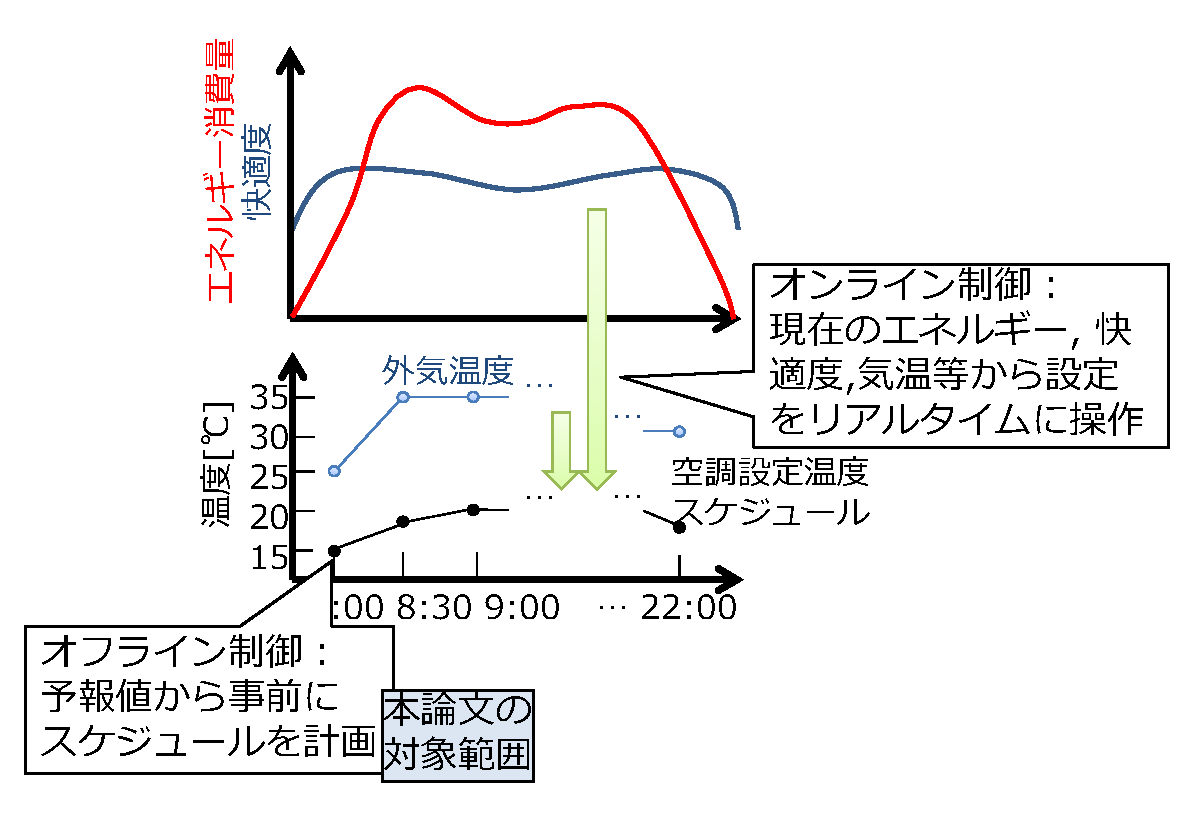
\includegraphics[width=0.6\textwidth,keepaspectratio=true]{fig/intro_offline.eps}
    \end{center}
    \caption{空調設定のオフライン制御とオンライン制御の関係}
    \label{fig::intro_offline}
\end{figure}

通常,ビルの空調設定は,ビル管理者により過去のエネルギー消費量データに基づいて季節や月・日単位で設定される.気象条件が通常と異なる場合やエネルギー消費量が目標値を超える恐れがある場合には,ビル管理者が空調設定を変更する.しかしながら,この運用はビル管理者のKKD(勘・経験・度胸)に頼ったものであることが多く,十分な節電ができない場合や,過度に節電してしまいオフィスの快適性の低下を招くことがある.また,十分な経験がない管理者には判断が難しい.そこで,空調設備の運用改善とビル管理者の業務省力化のために,空調設定計画の詳細なスケジュールを適切に決定する手法が必要である.

これまでに,空調設定計画の事前スケジューリングに対して,最適化手法を用いる方法が研究されている.単一目的の最適化手法を用いる方法として,1つは,室内の環境を快適に保つことができる空調機の設定の組合せのうちエネルギー消費量が最小になる組合せを探す,といったように快適性とエネルギー消費量のうちどちらか一方を制約条件とし,もう一方を目的関数に設定する方法がある\cite{Alhaider15, Ueda10, Xu13}.また,快適性とエネルギー消費量の重み付け和を目的関数として,1つの目的関数を持つ数理計画問題として解く方法がある\cite{Takagi11, Xiao17}.しかし,これらの単一目的の最適化手法では,重みや制約によってどの程度快適性もしくはエネルギー消費量が変化するかを事前に知ることができず,重みや制約値の決定が難しい.さらに,最適化によって得られる単一の最適解をそのまま適用するほかなく,例えば当日使用可能なエネルギー量に余力があり快適性を優先した設定としたい場合や,エネルギー量に制限が発生した場合などにスケジュールを調整することが困難である.そこで,エネルギー消費量と快適性を同時に追究する空調運用のため,多目的最適化による空調設定スケジュールの最適化手法が提案されてきた.

空調設定スケジューリングへの多目的最適化の適用事例として,エネルギー消費量ピークの抑制による電気料金の削減と快適な温度設定の維持を目的関数として適用した事例がある\cite{Zhang14}.この事例では,電気料金および室内温度をそれぞれ独立した目的関数として取り扱い,2つの目的の間のパレート解を探索している.一方で,目的関数はエネルギーや快適性を直接的に表現するものでなく,さらに目的関数の算出には簡素な数理モデルが採用されている.室内快適性とエネルギー消費量に影響するオフィスビルの様々な要素は複雑に相互作用するため,簡素な数理モデルでの表現が困難な場合がある.そのため,実用性の高い設定温度スケジュールを得るためには,高精度なシミュレーションに基づく最適化が必要になる.文献\cite{Bingham17, Pan16}では,住宅のエネルギー消費量および快適性の目的関数をEnergyPlusというビルシミュレータによって計算することによる改善が検討されている.このビルシミュレータを用いた多目的進化計算による最適化アプローチには,大きく2つの問題が存在する.1つ目は,住宅ではなくビルのような比較的大規模な建築物および設備に対する有効性の検証がなされていないことである.住宅と中~大規模のオフィスビルとの間には設備種類やその特性,使用条件に大きな違いがあるが,それらを考慮した最適化の実行の検討が必要である.2つ目はシミュレーションに時間がかかることである.1つの空調設定スケジュールの評価に数十秒の時間がかかるため,進化計算のような複数回の試行を前提とするアルゴリズムでは最適化の工程に多大な時間を要する.

\section{研究目的と方法}
本研究では,空調設備の運用改善とビル管理者の業務省力化のために,オフィスビルに対して空調設定スケジュールを多目的に最適化する方法論を構築し,その効果を検証することを目的とする.上述の従来手法における問題を打破するため,オフィスビルという比較的大規模な建築物に対して多目的最適化を適用する方法,および時間がかかるシミュレーションを用いて最適化することに対処する方法を構築し,それら手法の有効性を明らかにする.

まず,オフィスビルのうち一部屋の快適性とエネルギー消費量の目的関数を数理モデルで表現した空調設定スケジュールの多目的最適化問題を定式化し,この最適化問題に対して進化型多目的最適化手法を適用する最適化システムの構成を提案する.この最適化システムでは,空調設定スケジュールを設計変数とし,ある空調設定スケジュールの場合の室内の快適性と空調システムが消費するエネルギー量を数理モデルによって算出する.算出した快適性とエネルギー消費量という二つの目的を満たす空調設定スケジュールを解として多目的最適化によって探索するというコンセプトを提示する.この最適化システムでは,従来研究同様数理モデルを用いているため,ビル全体を数理モデル化することに対して困難さがある.そこで,室内快適性とエネルギー消費量の2つの目的関数を,ビルエネルギーシミュレータを用いて評価する手法を導入する.ビルエネルギーシミュレータは,複数ある室同士や,その室に設置された空調機との熱の相互作用を考慮して室内環境および空調機動作をシミュレートし,室内快適性とエネルギー消費量を詳細に算出することが可能である.これにより,空調設定スケジュールの多目的最適化というコンセプトのオフィスビルのような規模の大きい建築物および設備に対する有効性を検証する.
次に,シミュレータによる解評価を用いた場合に必要な計算コストへの対処を行い,より実用的な空調設定スケジュールを獲得するためのアプローチについて検討する.解評価に時間がかかるということは,大きく二つの問題を引き起こす.1つ目は,最適化工程に時間がかかるため,空調設定スケジュールを選択する時に精度の高い直近の気象情報を利用できず,気象予報誤差が生じた場合に獲得したスケジュールが最適ではなくなる問題である.これを解決するため,外気温予報誤差を考慮した目的関数を追加することにより気象予報誤差に対するロバストな空調設定スケジュールを獲得する手法について検討する.2つ目は,解評価に時間がかかるために,進化計算のように最適化に多数の個体の評価を必要とする手法では評価回数を通常より少なくせざるを得ず,最適化をするための十分な回数の評価ができない問題である.この問題を解決するために,シミュレーションを用いた解評価を,より計算コストが低いサロゲートモデルによる評価に置き換えることで,評価時間を短縮し進化計算による最適化を加速させる手法について検討する.

本研究で提案する方法の効果は,1万[$m^2$]規模のオフィスビルモデルに対して適用することにより検証する.これは,業務部門の最終エネルギー消費のうち,オフィスビルの割合が最も高いこと\cite{EDMC15},オフィスビルの中でも1万[$m^2$]以上のビルのエネルギー消費の割合が約7割と高いことが理由である\cite{BEMA20,EDMC15,Fudoken19}.本研究では,対象ビルモデルとして,省エネルギービルの基準であるZEB\footnote{ZEB…net Zero Energy Building.新築・改修の設計段階において,年間のエネルギー消費量を基準値以下にしたビルのこと}とZEBを実現するための設計手法や技術採用の指針について定義される「ZEB設計ガイドライン」にモデルケースビルとして例示されている中規模オフィスビル\cite{ZEB18}を模擬したシミュレーションモデルを構築する.ガイドラインで示された一般的なオフィスビルを模擬することで,より現実的な問題に対する効果検証を可能とする.
また,本研究で提案する方法の効果は,同様に空調設備を用いる他の用途のビルや工場などでも同様に期待できると考えられる.一方で,建物用途が異なると,エネルギー使用状況が大きく異なること\cite{Kanto11},オフィスビルを対象として本研究で想定していた設計変数・快適性に関する目的関数を変更しなければならない可能性があることから,本研究ではオフィス以外の建物に関する検討はスコープ外とする.

% ビル空調スケジュール最適化の分類
% 目的数:単目的/多目的,ロバスト性の考慮有無
% (規模:住宅~小規模/中~大規模,モデル:数理モデル/シミュレータ)でマトリクス作る
\begin{figure}[ht]
    \begin{center}
        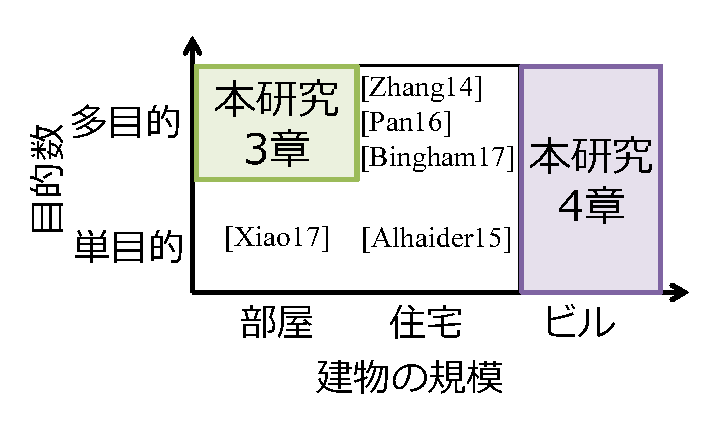
\includegraphics[width=0.6\textwidth,keepaspectratio=true]{fig/intro_position_objective.eps}
    \end{center}
    \caption{本研究の3章および4章の位置付け}
    \label{fig::intro_position_objective}
\end{figure}

\begin{figure}[ht]
    \begin{center}
        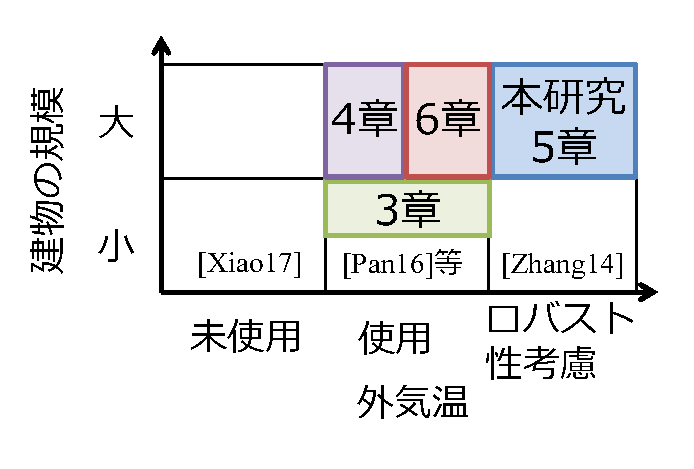
\includegraphics[width=0.6\textwidth,keepaspectratio=true]{fig/intro_position_robust.eps}
    \end{center}
    \caption{本研究5章の位置付け}
    \label{fig::intro_position_robust}
\end{figure}

\begin{figure}[ht]
    \begin{center}
        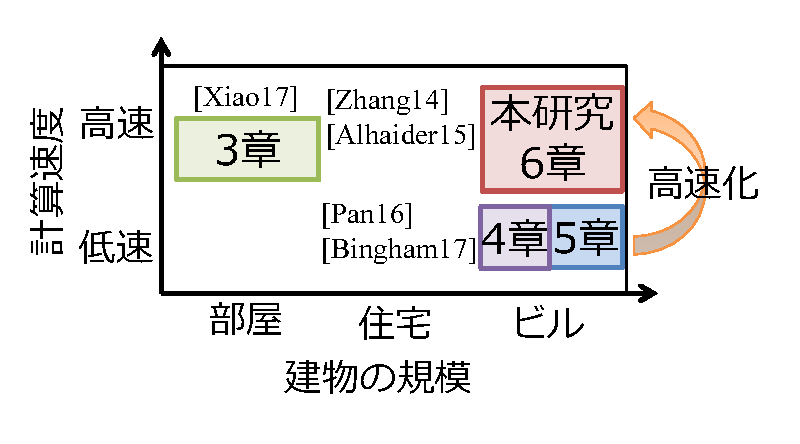
\includegraphics[width=0.6\textwidth,keepaspectratio=true]{fig/intro_position_speed.eps}
    \end{center}
    \caption{本研究6章の位置付け}
    \label{fig::intro_position_speed}
\end{figure}

\section{研究の位置付け}
上述の従来法と本研究におけるアプローチを,まず対象とするビル規模と目的数で分類したものを\figref{fig::intro_position_objective}に示す.目的関数の数を単目的とすると,上述のように重みや制約値の決定が難しく,また調整が困難であり,現場適用に課題がある.一方で目的関数の数を多目的とすると,どの程度快適度を犠牲にすることでエネルギー消費量を良い値にできるといったトレードオフ関係を考慮しつつ,適切なスケジュールを選択することができる.そのため,単一目的最適化で生じていた重みや制約値の調整の問題を解決できる.また,運用に変更があった場合にもエネルギー消費量や快適度の異なる他のスケジュールを適用することが容易であり,実利用に対して適した方法といえる.一方,対象ビル規模は,適用先によってさまざまであるが,一般に規模が大きくなるにつれ,大規模な熱源設備や空調設備が必要とされ,制御対象の面積・部屋数が増加するため,エネルギー消費量や快適度の予測および最適化が困難になる傾向にある.本研究では,中~大規模オフィスビルの空調設定スケジュールの最適化を対象とする.このようなビルでは,場合によってビルの部屋およびテナント単位の最適化も必要とされることから,まずオフィスビルの1部屋を対象として空調設定スケジュールの多目的最適化を行うコンセプトを提示する.その後,オフィスビル全体の多目的・単目的の空調設定スケジュール最適化の手法および結果について議論する.
次に,対象ビル規模と外気温の取り扱いで分類したものを\figref{fig::intro_position_robust}に示す.通常,ビルのエネルギー消費量および室内快適度には外気温が大きな影響を与える.計算を単純化するため,外気温を考慮しない数理モデルで最適化を行うアプローチが従来法にある\cite{Xiao17}.しかし,モデルによる目的関数算出を正確に行うためには外気温を考慮して目的関数計算する手法の採用が必要である.さらに実際には外気温が予報値に対して誤差を持つことから,これを考慮することでより実用性の高いスケジュールを獲得するアプローチがある.従来法\cite{Zhang14}ではモンテカルロ法により生成した複数の外気温予報シナリオの結果の発生確率による加重平均値を評価値として最適化するアプローチをとっていた.しかしながら,この手法では,1つの解を評価するためにシナリオ数の分の目的関数計算が必要であること,平均値を評価値とするため獲得できるスケジュールは予報値で最適化した結果に近い値に収束すること,ロバスト性を考慮せず目的関数値を良くした解は同時には得られないこと,などの問題があった.本研究では,実際の気象予報誤差データから上方・下方予報誤差のうち$\pm 2\sigma$の誤差分布までを考慮し,ロバスト性も目的とした多目的最適化アプローチによる空調設定スケジュールの最適化を5章にて実施している.これらのようなアプローチをオフィスビルに対して適用した例はこれまでにない.既設ビルのうち多くを占めるオフィスビルにおいて,この手法が有効であることを検証する.
さらに,対象ビル規模と計算速度について分類したものを\figref{fig::intro_position_speed}に示す.通常,対象ビル規模が大きくなるほど,快適性およびエネルギー消費量を算出するために計算しなければならない空調設備モデルや室モデルの数が増加するため,計算速度も低下する傾向にある.さらに,部屋や住宅の単位であればその計算モデルは数理モデルで記述が容易な規模であるが,規模の大きなビルになるとその計算モデルを逐一記述することは困難になってくる.そこで,ビルの構造や設備等の情報からモデルを定義し計算を行うシミュレータの利用が必須となる.シミュレータの内部構造は詳細な多数の数理モデルがビルモデルに合わせて結合されたものであることから,計算時間は多くかかることが一般的である.そこで,目的関数計算をサロゲートモデルで近似することが行われる.従来法\cite{Tresidder12}では,クリギング法を用いて設計変数ベクトルから目的関数値を直接近似するサロゲートモデルを用いる方法が考案されている.しかしながら,クリギング法では変数の数が多い場合に近似性能が悪化してしまうこと,近似対象の関数が連続値であることを想定した手法であるため,制約違反量のような非線形関数の近似は困難であることが問題であった.本研究では,シミュレータの出力する時系列データをNNを用いて近似し,時系列データを用いて目的関数計算する手法を6章にて提案する.本手法によって多変数データの近似が可能となるだけでなく,得られた時系列データから目的関数・制約違反量を計算することで非線形な関数値も推測可能である.

\begin{figure}[ht]
    \begin{center}
        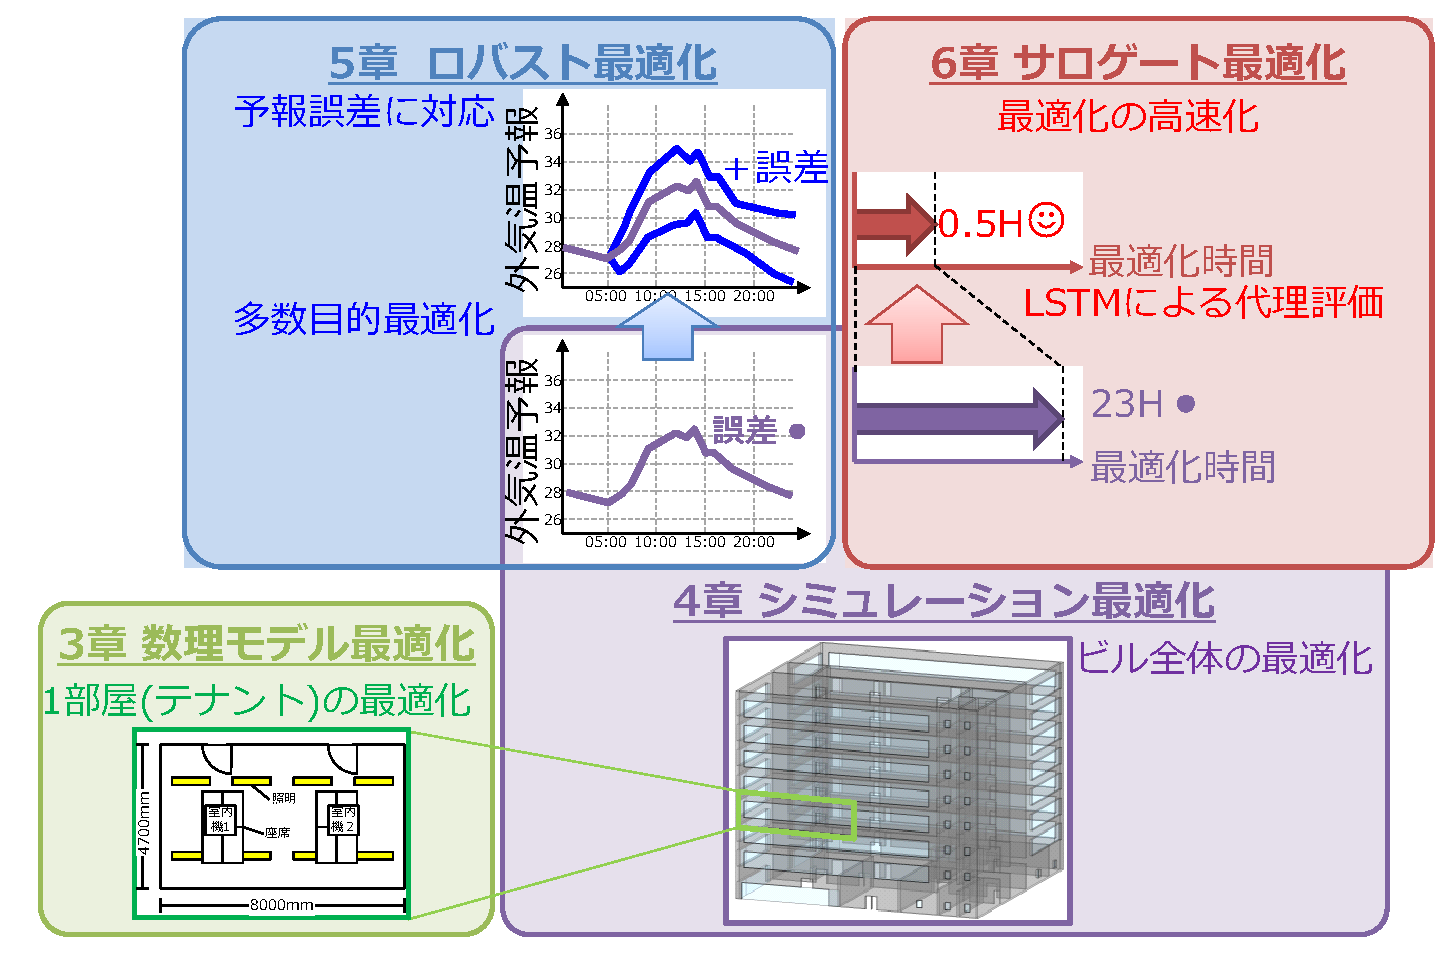
\includegraphics[width=1.0\textwidth,keepaspectratio=true]{fig/intro_bigpicture.eps}
    \end{center}
    \caption{本論文の全体像}
    \label{fig::intro_bigpicture}
\end{figure}

\section{本論文の構成}
%本論文の構成を以下に示す.
以下,2章では,本論文の展開に必要な進化計算に関する基礎的事項について述べ,3章以降に本論文で提案する方法について述べる.本研究で提案する方法の全体像を\figref{fig::intro_bigpicture}に示す.
2章では,多目的最適化問題と,その進化計算による解法について説明する.まず,多目的最適化問題とその解を求めるための基本的アプローチについて説明する.次に,多目的最適化の解探索手法として用いられる進化計算について,一般的な計算過程と解候補の生成方法,選択方法について説明する.その後,代表的な多目的最適化のための進化計算手法としてNSGA-IIおよびOMOPSOを取り上げ,そのアルゴリズムについて説明する.また,ほとんどの実問題が備える制約条件の考慮の方法について説明する.
3章では,オフィスビルの一部屋に対する空調設定スケジュール最適化問題を,従来行われてきた数理モデルにより定式化し,進化計算手法により最適化する手法を示す.空調設定スケジュール最適化問題の設計変数,目的関数,制約条件を定義し,これらの算出に必要な物理的要素,設備パラメータについて説明する.また,快適性の評価において重要な評価尺度であるPMVについて説明する.そして,この問題に対して進化計算を適用した場合に得られるパレート最適解集合とそのスケジュールの時系列データの分析を行う.
4章では,中規模ビルに対するシミュレーションモデルを構築し,シミュレーションモデルに基づいた評価を用いた進化計算手法により多目的最適化をする方法を示す.最適化対象とする中規模オフィスビルのフロアレイアウト,躯体・構造,壁・窓材料や各種設備について説明したのち,このビルを運用した場合のエネルギー消費量および快適度を算出するビルエネルギーシミュレーションモデルを構築する方法について詳細を述べる.また,このシミュレーションモデルによるシミュレーション結果から3章で述べた空調設定スケジュール最適化問題の目的関数,制約条件を計算する手順について説明する.その後,シミュレーションモデルによる評価に基づく多目的最適化によって獲得されたパレート最適解と,従来の設定温度を一定値として運用した結果との比較を行う.加えて,提案法の妥当性を検証するために,快適性の制約条件式を設けない場合との比較,快適性を目的ではなく制約とした場合の単一目的最適化結果との比較,他の多目的最適化手法による探索結果との比較,OMOPSOのアルゴリズム上の工夫の効果の比較を行う.
5章では,外気温の予報誤差に対してロバストな空調設定スケジュールを獲得する手法を示す.まず,気象庁が発表する外気温予報値と実績値を用いて実際の外気温予報精度を分析し,予報誤差を再現するシミュレーション用外気温データの設計手法を説明する.設計した予報誤差を含む外気温データを用いて,外気温予報誤差に対するロバスト性を示す2つの目的関数を定式化する.快適性・エネルギー消費量の2つの目的に加えて,ロバスト性を示す2つの目的関数を含む4目的の空調設定スケジュール最適化問題に対し,進化計算を用いてパレート最適解を探索する.獲得された外気温予報に対するロバストな空調設定スケジュールについて,従来の快適性・エネルギー消費量のみを考慮した場合の探索結果との比較を行う.さらに,4目的という多数目的最適化のクラスとなったロバスト空調設定スケジュール最適化問題に対して,複数の多目的・多数目的最適化手法による探索を試行し性能比較を行う.
6章では,シミュレータをサロゲートモデルにより簡素に代替することによる進化計算の総計算時間の短縮手法について提案する.4章で提案したシミュレーションモデルの入出力を,Recurrent Neural Network(RNN)の1つであるLSTMを用いて代替する手法の概要を説明する.また,LSTMによるサロゲート評価器の入出力,ネットワーク構成および学習手法を説明する.シミュレータの入出力データを学習データとして訓練したサロゲート評価器の予測精度について分析する.また,このサロゲート評価器を用いて多目的最適化した結果得られたパレート最適解について,サロゲート評価器とシミュレータそれぞれの出力結果を比較する.さらに,サロゲート評価器を用いた場合の最適化計算時間についてシミュレータとの比較を行い,サロゲート評価器による高速化の効果について分析する.加えて,同様の評価回数でもより良好な解を探索する,進化計算アルゴリズムの改良手法DOMOPSOを考案し,サロゲート評価器による多目的最適化問題に対して適用した結果について考察を行う.
最後に7章で本論文をまとめ,今後残された課題について述べる.

\chapter{多目的最適化}
\label{chap::multiobjective}

\hspace{1zw}この章では多目的最適化問題の概要と,進化計算による解法について記述する.

\section{問題定義}
ある目的の達成度を,値の小さい(もしくは大きい)ほうが高いものとして関数化したものを目的関数とよぶ.多目的最適化問題とは複数の目的関数集合$\vec{f}(\vec{x})$を最小化(もしくは最大化)する解$\vec{x}$を求める問題である.多目的最適化問題は,以下の式で表現される.

\begin{align}
     & 目的関数:\mbox{Minimize/Maximize} \quad \vec{f}(\vec{x}) = \{f_1(\vec{x}), f_2(\vec{x}),\cdots,f_m(\vec{x})\} \\
     & 制約条件:\mbox{Subject to} \quad ~~~~~~~~~~~~~ \vec{x} \in X
\end{align}
ここで,$m$は目的の数,$\vec{x}$は設計変数(操作可能な変数,決定変数とも呼ぶ),$f_i(\vec{x}) \quad (i=1, 2,\cdots,m)$は設計変数$\vec{x}$から算出されるある目的の達成度を示す目的関数,$X$は設計変数$\vec{x}$の実行可能領域(操作可能範囲)である.


目的の数$m=1$の場合,単目的最適化問題もしくは単一目的最適化問題と呼ぶ.単一目的最適化問題では,真の最適解は一つに定まる.一方,本研究では,上の式で定式化され,目的関数が複数$m \geq 2$であり,複数の目的の間に1つ以上のトレードオフの関係がある多目的最適化問題を取り扱う.$m=2$目的の最小化の目的関数空間を\figref{fig::theory_moo}に例示する.このような問題では,全ての目的関数を同時に最小化することはできない.そこで,操作可能範囲内でこれ以上全ての目的を同時に改善できない解(=パレート最適解)を解候補として定義する.パレート最適解は1つには定まらず解の集合となる.パレート最適解集合からなる超平面を目的関数空間上で表したものをパレートフロントと呼ぶ.多目的最適化とは,パレートフロントのうち少なくとも1点を求めることである.

また,制約を表す実行可能領域$X$は制約関数集合$\vec{g}(\vec{x}) \leq \vec{0}$で表される.ただし,$\vec{g}(\vec{x})=\{g_1(\vec{x}), g_2(\vec{x}),\cdots,g_p(\vec{x})\}$であり,$p$は制約の数である.$p$個の全ての制約を満たす解は実行可能解,一つでも制約を満たさない解は実行不可能解と呼ばれる.

\begin{figure}[ht]
    \begin{center}
        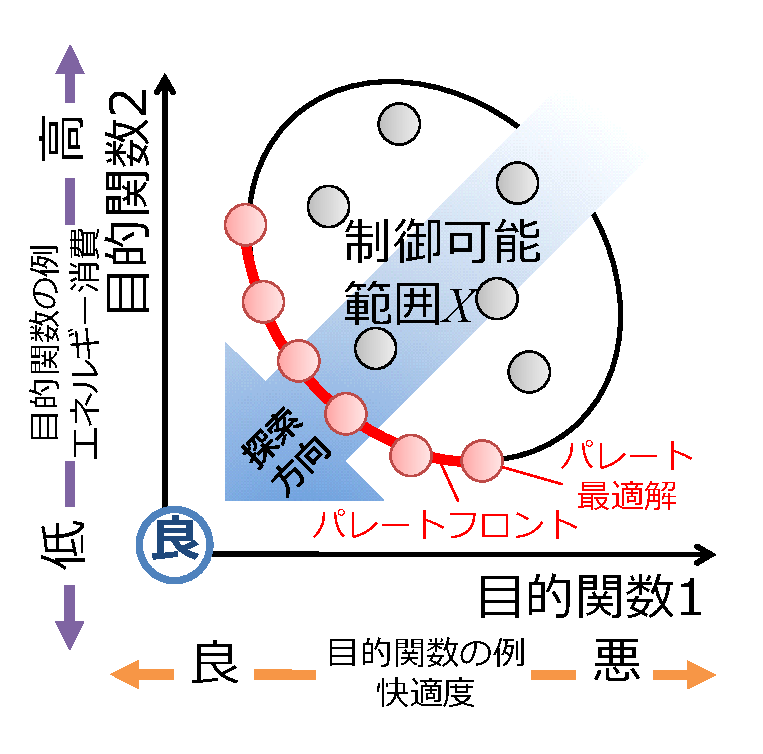
\includegraphics[width=0.6\textwidth,keepaspectratio=true]{fig/theory_moo.eps}
    \end{center}
    \caption{多目的最適化の概念}
    \label{fig::theory_moo}
\end{figure}

多目的最適化問題を解くにあたり重要な概念として,解の優越関係(あるいは支配)がある.2つの解候補を比較したときに,一方が他方に対して全ての目的関数で良い値を持つ場合,その解は他方を優越(dominate, 支配)するという.逆に,全ての目的関数で悪い目的関数値を持つ解は,他方に対し被優越(dominated, 非支配,劣っている)解という.例えば$m=2$目的の最小化問題の\figref{fig::theory_dominate}において2つの解候補$\vec{x}$と$\vec{y}$を比較したときに,$\vec{x}$は$\vec{y}$に対して目的関数1についても目的関数2についても小さい値=良い値であるため,$\vec{x}$は$\vec{y}$を優越することがわかる.また,2つの解候補$\vec{x}$と$\vec{z}$を比較すると,$\vec{x}$は$\vec{z}$に対して,目的関数1については小さい値=良い値だが,目的関数2については大きい値=悪い値であるため,$\vec{x}$は$\vec{z}$を支配しない.また,$\vec{z}$も$\vec{x}$を支配しない.これを非劣もしくは非支配の関係という.\figref{fig::theory_moo}に示すパレート最適解集合は全解集合$X$の非劣解集合であり,多目的最適化では探索中に生成した解集合の中における非劣解集合を獲得することがゴールである.\figref{fig::theory_dominate}に図示する全ての点を生成した解集合だとすると,赤の点が多目的最適化の結果として出力する非劣解集合である.

\begin{figure}[htbp]
    \begin{center}
        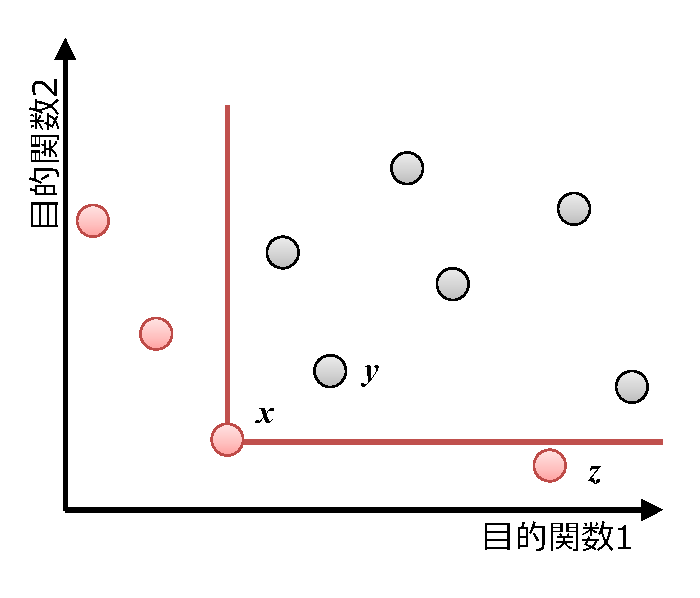
\includegraphics[width=0.6\textwidth,keepaspectratio=true]{fig/theory_dominate.eps}
    \end{center}
    \caption{解の優越関係}
    \label{fig::theory_dominate}
\end{figure}


\section{進化計算による解法}
\subsection{進化計算}\label{subsec::ec}
進化計算(Evolutionary Computation,進化的計算,進化的アルゴリズムとも呼ぶ)とは,生物の進化の過程や群れの動きの様子を模擬する解の集合を利用することによって新たな解を探索する手法の総称である.進化計算の特徴として,以下が挙げられる.
\begin{itemize}
    \item 進化計算はメタヒューリスティクスの一つであり,特定の計算問題に依存しないアルゴリズムである.多様な問題に対して汎用的に対応でき,問題の特性が未知であることがほとんどである実問題に対しても,問題をブラックボックスとして扱って最適化できる.
    \item 解集合を用いて探索する多点探索手法である.多目的最適化では,上述のように最終的にパレートフロントを近似するパレート解集合を求める必要がある.解集合を用いて探索する進化計算は,多目的最適化におけるパレート最適解集合を一回の探索で求めることができ,目的間のトレードオフ関係を考慮した解の意思決定を支援できる.
    \item 確率的に探索する手法である.数理最適化法では問題の厳密解を求めることができるが,進化計算では確率的な探索であるため厳密解を発見する保証はない.厳密解に近い近似解を求めることになる.
\end{itemize}
最も代表的な進化計算は,遺伝的アルゴリズム(GA, Genetic Algorithms)である.GAは生物の進化の過程を模擬したアルゴリズムである.GAは解の候補を生物の個体に見立てて,個体の交叉,淘汰,突然変異による世代交代を模擬する計算を行うことで良好な解を探索する.また,同様に代表的な進化計算として粒子群最適化(PSO, Particle Swarm Optimization)がある.PSOは解集合を魚や鳥などの群れになぞらえ,各個体を群れ全体で方向性をもたせて飛翔させることによって解探索する.この他にも焼きなまし法(SA, Simulated Annealing), 差分進化(DE, Differential Evolution),蟻コロニー最適化(ACO, Ant Colony Optimization), カッコー探索(CS, Cuckoo Search)など様々な手法が提案されている.

進化計算には様々な手法があるが,どの手法も概ね\figref{fig::theory_flow}に示すフローで探索する.ここでは進化計算の探索フローにおける各項目を説明する.

\begin{figure}[ht]
    \begin{center}
        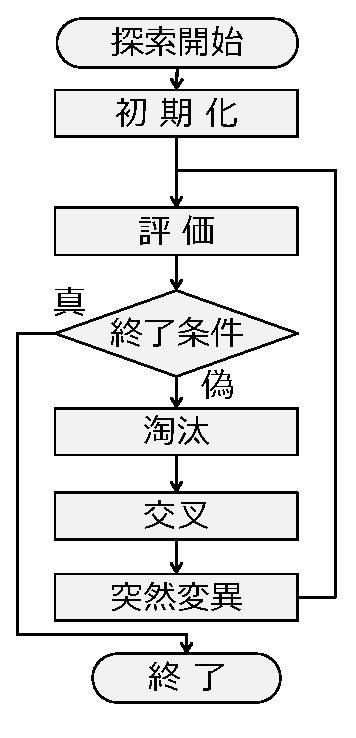
\includegraphics[width=0.3\textwidth,keepaspectratio=true]{fig/theory_flow.eps}
    \end{center}
    \caption{一般的な進化計算アルゴリズムのフロー}
    \label{fig::theory_flow}
\end{figure}

\subsubsection{初期化}
探索に用いる初期解集合を生成する.通常は解の変数それぞれを取りうる範囲の中で一様乱数を用いて決定する.一方で,実問題では通常使用する値やデフォルトの設定値などが存在するため,それを変数とした複数の初期解を用いることもある.また,進化計算では解を個体,解集合を個体群と呼ぶことがある.

\subsubsection{評価}
個体群に含まれる各個体の変数値を使って目的関数値を計算し,個体の評価を行う.


\subsubsection{淘汰}
個体群の中から,次世代に残す個体を選択することを淘汰(または選択)と呼ぶ.淘汰を行う方法にはいくつかの種類があるが,基本的には目的関数値の値の良い解を優先的に次世代に残す方策をとる.進化計算では,選択された解を親(または親個体)と呼ぶことがある.多目的最適化の場合は目的関数が複数あるため,上述の優越関係を用いて淘汰する.最も一般的に用いられる淘汰の方法として,非支配ソートと呼ばれる方法\cite{Deb02}がある.非支配ソートでは,解集合を支配されないレベルでランク分けし,ランクの上位から順序付けする手法である.\figref{fig::theory_rank}に非支配ソートの概念図を示す.解集合のうちどの解にも支配されていない解(非劣解)をランク1として解集合から取り出す.残った解集合の中から,同様に非劣解を取り出してランク2とする.解集合から解がなくなるまでこれを繰り返す.このように解集合をランクで分類し,ランクの値が小さいものほどよい解であると判定して次世代に残す.

\begin{figure}[ht]
    \begin{center}
        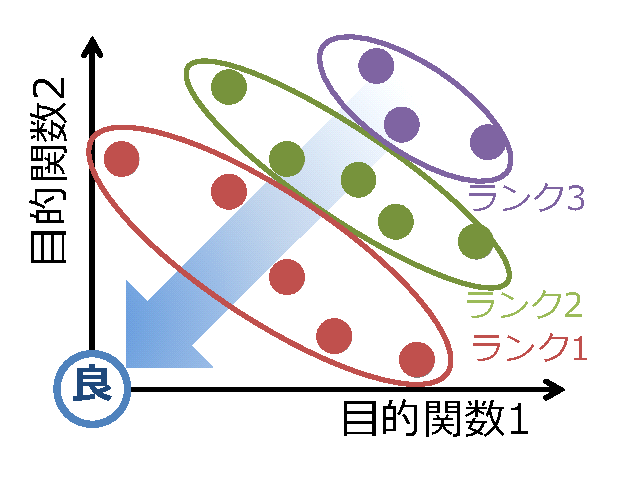
\includegraphics[width=0.6\textwidth,keepaspectratio=true]{fig/theory_rank.eps}
    \end{center}
    \caption{被支配ソートの概念図}
    \label{fig::theory_rank}
\end{figure}

\subsubsection{交叉}
個体群から親個体を選択し,親個体の設計変数の情報をかけ合わせて新たな解を生成する操作を交叉(Crossover)と呼ぶ.進化計算では,交叉によって生成される解を子(または子個体)と呼ぶことがある.交叉方法にも設計変数の種類などによって様々な種類が存在する.ここでは主にGAで用いられる実数値変数用の交叉方法として単峰性正規分布交叉(Unimodal Normal Distribution Crossover, UNDX)\cite{Kita99, Ono97}, Simulated Binary Crossover(SBX)\cite{Agrawal95},さらに粒子群最適化(Particle Swarm Optimization, PSO)\cite{Kennedy95}で用いられる交叉について説明する.
\begin{itemize}
    \item UNDX\cite{Kita99, Ono97}\\
          UNDXは親個体を3つ選択し,親個体集合の重心から正規分布で子を生成する手法である.UNDXによる解の生成方法を\figref{fig::theory_undx}に例示する.UNDXは,親個体群から3つ($\vec{x}_0, \vec{x}_1, \vec{x}_2$)の個体を選択した後,子個体$x_c$を以下の式に従って生成する.
          \begin{align}
              \vec{x}^{c} & = \vec{x}_p + \xi \vec{d}_{01}+D \sum_{i=1}^{n-1} \eta_i \vec{e}_i
          \end{align}
          ここで,$\vec{x}_p$は$\vec{x}_0$と$\vec{x}_1$の中間点$\vec{x}_p = (\vec{x}_0+\vec{x}_1)/2$, $\vec{d}_{01}=\vec{x}_0-\vec{x}_1$, $\xi$は$N(0, \sigma_\xi)$に従う乱数,$\eta_i$は$N(0, \sigma_\eta)$に従う乱数,$D$は$\vec{x}_p$から$\vec{x}_2$へのベクトルの大きさ$|\vec{d}_v| = |\vec{x}_2-\vec{x}_p|$, $\vec{e}_i$は$\vec{d}_{01}$に直交する正規直交基底$\vec{d}_{v}$の基底ベクトルである.
          この式により, 親個体$\vec{x}_0, \vec{x}_1$の中間点を中心として,$\vec{x}_0, \vec{x}_1$方向,$\vec{x}_2$方向それぞれに広がる範囲に乱数で子個体を生成する.
          \begin{figure}[ht]
              \begin{center}
                  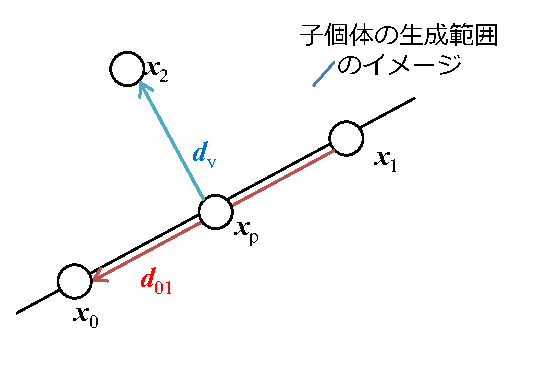
\includegraphics[width=0.5\textwidth,keepaspectratio=true]{fig/theory_undx.eps}
              \end{center}
              \caption{UNDXによる交叉}
              \label{fig::theory_undx}
          \end{figure}

    \item SBX\cite{Agrawal95}\\
          SBXは,親個体2つを選択し,交叉率(Crossover Probability, $P_c$)および分布度(Distribution Index, $\eta_c$)の2つのパラメータにより,確率的に親個体の周囲に新たな解を生成する手法である.SBXは個体の持つ各変数について,1/2の確率で同じ値とし,1/2の確率で次式で算出される値となる.
          \begin{align}
              \beta_i  & =
              \begin{cases}
                  (2u_i)^{\frac{1}{\eta_c+1}} ~~~~~~~~ \mbox{if} \quad u_{i} \leq 0.5, \\
                  (\frac{1}{2(1-u_i)})^{\frac{-1}{\eta_c+1}} \quad \mbox{otherwise},
              \end{cases}                                  \\
              x_i^{a'} & = 0.5 \{(1+\beta_i)x_i^a + (1-\beta_i)x_i^b \}, \\
              x_i^{b'} & = 0.5 \{(1-\beta_i)x_i^a + (1+\beta_i)x_i^b \}.
          \end{align}
          ここで,$x_i^a$, $x_i^b$は選択した2つの親個体$\vec{x}^a$, $\vec{x}^b$の$i$番目の変数,$x_i^{a'}$, $x_i^{b'}$は生成された子個体の$i$番目の変数,$\beta_i$は$i$番目の変数に対する拡散係数,$u_{i}$は$[0,1)$のランダムな値を表す.SBXは,最初に分布度$\eta_c$に基づいて拡散係数$\beta_i$を算出する.また1/2の確率で拡散係数$\beta_i$の符号を反転する.その拡散係数をもとに2つの親個体$\vec{x}^a$, $\vec{x}^b$から子個体の変数を算出する.分布度$\eta_c$は小さいほど周辺の広い範囲に解を生成し,値が大きいほどもとの設計変数近くに解が生成される.

    \item PSO\cite{Kennedy95}\\
          PSOによる交叉を\figref{fig::theory_pso}に例示する.PSOでは,解を粒子に見立て,変数を粒子の現在位置とする.粒子の速度と,個体群(粒子群)のうち良好な粒子方向へのベクトルを\Eqref{eq::theory_pso_velocity}および\Eqref{eq::theory_pso_position}の式により足し合わせることで,次世代の粒子の位置(=変数)を生成する.PSOではこの操作を交叉の代わりに飛翔と呼ぶ.
          \begin{align}
              \vec{v}^{g+1} & = w\cdot \vec{v}^g + c_1 \cdot r_1 (\vec{x}_{pbest}-\vec{x}^g) + c_2 \cdot r_2 (\vec{x}_{gbest} - \vec{x}^g)
              \label{eq::theory_pso_velocity}
              \\
              \vec{x}^{g+1} & = \vec{x}^g + \vec{v}^{g+1}
              \label{eq::theory_pso_position}
          \end{align}
          ここで,$\vec{x}^g$と$\vec{v}^g$は,世代$g$の設計変数空間における粒子の位置と速度である.また,$w$,$c_1$,$c_2$は任意の重み係数,$r_1$と$r_2$は$[0, 1)$の一様乱数である.$\vec{x}_{pbest}$はパーソナルベストの位置で,$\vec{x}_{gbest}$はグローバルベストの位置である.パーソナルベストとは,ある粒子$\vec{x}^g$がこれまで飛翔してきた中で最も目的関数の評価値の高い粒子である.また,グローバルベストとは,ある世代$g$の粒子群の中で最も評価値の高い粒子である.
          \begin{figure}[ht]
              \begin{center}
                  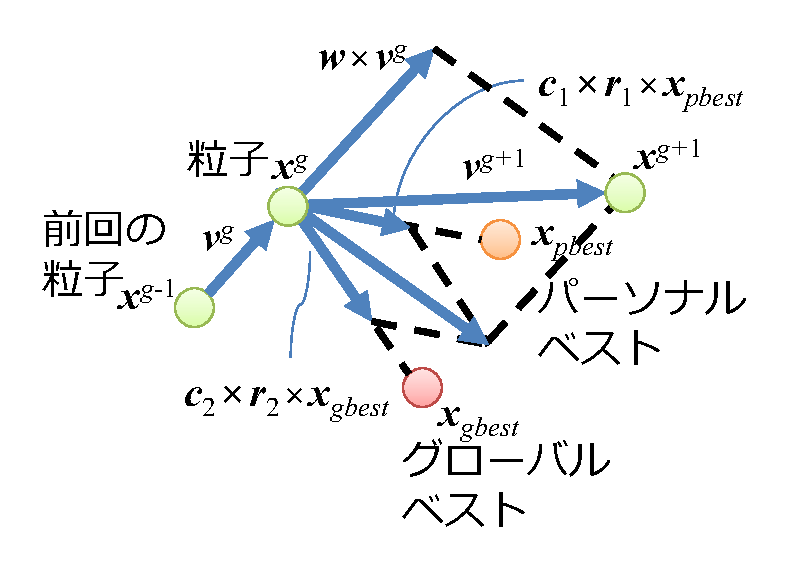
\includegraphics[width=0.5\textwidth,keepaspectratio=true]{fig/theory_pso.eps}
              \end{center}
              \caption{PSOによる交叉}
              \label{fig::theory_pso}
          \end{figure}

\end{itemize}

交叉によって生成された解の変数が変数の取りうる範囲[$x^{min}, x^{max}$]を超過した場合,その解は実行不可能解となってしまうため,超過した変数については実行可能とするよう,境界値まで引き戻す操作を加えることがある.

\subsubsection{突然変異}
交叉によって生成した子個体群の一部の設計変数に対してランダムに操作を加えることを突然変異(Mutation)とよぶ.突然変異には一様突然変異,非一様突然変異などの種類がある.また,設計変数が2値か実数値かによってもいくつか種類がある.ここでは,一般的な一様突然変異,後述のOMOPSOで採用される非一様突然変異,実数値を用いた進化計算アルゴリズムでよく用いられるPolynomial Mutation(PM)について説明する.

\begin{itemize}
    \item 一様突然変異\\
          一様突然変異では,設計変数値ごとに突然変異確率$p_m$で一様乱数値を加える,もしくは一様乱数値に置き換える操作を行う.一様乱数の範囲は,設計変数の取りうる範囲全体$[x^{min}, x^{max}]$や,範囲の1/4を上下に加える$[-0.25(x^{max}- x^{min}), 0.25(x^{max}- x^{min})]$など,いくつかのパターンがある.

    \item 非一様突然変異\cite{Esquivel03}\\
          非一様突然変異では,世代数$g$によって設計変数空間における変異域を変更する.OMOPSOの例では,設計変数値ごとに突然変異確率$p_m$で,次式により新たな$\vec{x}'^{g+1}$を得る非一様突然変異が用いられる.
          \begin{align}
              \small
              x'^{g+1}_i & =
              \begin{cases}
                  x^{g+1}_i+\Delta(g, x^{max}-x^{g+1}_i), \text{if } r_3 < 0.5 & \\
                  x^{g+1}_i-\Delta(g, x^{g+1}_i-x^{min}), \text{otherwise}     & \\
              \end{cases}
              \label{eq::theory_mutation_nonuni}
          \end{align}
          ただし,$\Delta(g, y)$は変異量であり次式で算出する.
          \begin{align}
              \Delta(g, y) = y\cdot\left(1-r^{\left(1-\frac{g}{g_{max}}\right)^b}_4\right)
          \end{align}
          ここで,$x^{g+1}_i$は粒子$\vec{x}^{g+1}$の$i$番目の設計変数の要素,$g_{max}$は総世代数,$r_3$と$r_4$は$[0, 1)$の一様乱数,$b$は変異量を変化させるパラメータである.

    \item PM\cite{Deb96}\\
          PMは突然変異確率(Mutation Probability, $P_m$)と分布度(Distribution Index, $\eta_m$)の2つのパラメータにより突然変異範囲と数を制御する,実数値変数用の突然変異法である.また,世代数によって突然変異確率が変わらない一様突然変異の手法の一つである.突然変異確率$P_m$は解の変数$x_i$に対して,突然変異を適用する確率である.PMによる突然変異後の変数は以下の式で算出する.
          \begin{align}
              \delta_i & =
              \begin{cases}
                  ((2u_{i3}+(1-2u_{i3})(1-\frac{x_i-x_i^{lower}}{\Delta_{i,max}}))^{\eta_m+1})^{\frac{1}{\eta_m+1}-1}          & if \quad u_{i3} \leq 0.5, \\
                  (1-(2(1-u_{i3})+2(u_{i3}-0.5)(1-\frac{x_i^{upper}-x_i}{\Delta_{i,max}}))^{\eta_m+1})^{\frac{1}{(\eta_m+1)}}) & otherwise,                \\
              \end{cases}
              \label{eq::theory_mutation_pm}
          \end{align}
          \begin{align}
              \Delta_{i,max} = x_i^{upper}-x_i^{lower} \\
              x_{i}' = x_{i}' + \delta_i \Delta_{i,max}
          \end{align}
          ここで,$\Delta_{i,max}$は$i$番目の変数の範囲の大きさ,$\delta_i$は$i$次元目の変異係数,$u_{i3}$は$[0,1)$の一様乱数を示す.変異係数$\delta_i$は変数の現在の値と上下限値を考慮して変数の取りうる範囲を超過しないように決定される.

\end{itemize}

PMは変数の取りうる範囲を超過しないよう変異量が決定されるが,一様突然変異や非一様突然変異では変数の取りうる範囲を超過する場合がある.その場合は交叉と同様に超過した変数を境界値まで引き戻す操作を加えることがある.

\subsubsection{終了条件}
進化計算の上述のサイクルを終える条件を定める.最も単純な終了条件は世代や目的関数の評価回数の最大値を定めておき,最大値を超過したら探索を終える,という条件である.その他にも,解集合内の目的関数値が一定以上となった場合や,一定世代改善されなかった場合などに終了する手段がある.

\subsection{NSGA-II\cite{Deb02}}\label{subsec::NSGAII}
NSGA-II(Fast Elitist Non-dominated Sorting Genetic Algorithm)は,GAを用いて多目的最適化問題を解くことができるような工夫を加えた手法であり,多目的進化型アルゴリズムの中でも特に代表的なアルゴリズムである.NSGA-IIのアルゴリズムの流れを以下の\figref{fig::theory_nsga2}に示す.
\begin{figure}[ht]
    \begin{center}
        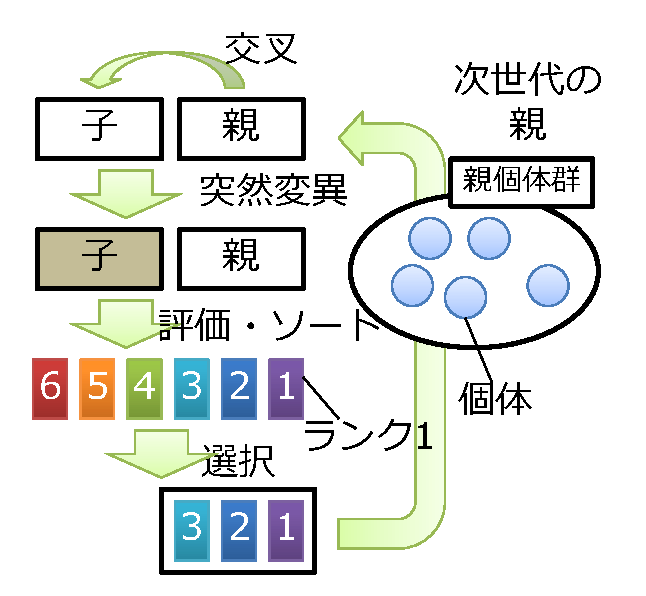
\includegraphics[width=0.6\textwidth,keepaspectratio=true]{fig/theory_nsga2.eps}
    \end{center}
    \caption{NSGA-IIのアルゴリズムのフロー}
    \label{fig::theory_nsga2}
\end{figure}
NSGA-IIは,特に選択(淘汰)において特徴的な操作を行う.NSGA-IIは各世代の解集合を非支配ソートを用いてランキングする.ランク値の良いものから順に次世代の親個体群とする.同一ランクの中で順位付けを行う場合,後述の混雑度の値が大きい順に選択する.混雑度は値が大きいほど周囲に解が存在しないことを示すため,疎な領域から順に解を選択することになる.このようにして得られた親個体群から,交叉によって親個体群と同数の子個体群を生成し同様に淘汰を繰り返すことで,解の進化を行う.

\subsubsection{混雑度}
混雑度(CD: Crowding Distance)は,目的関数空間における解の分布の密集度を表す指標である.混雑度の概念を以下の\figref{fig::theory_crowding_distance}に示す.混雑度は,同一のランク内である解集合をある一つの目的関数値順にソートし,両隣の解の目的関数の差を足し合わせた値である.\figref{fig::theory_crowding_distance}における解$\vec{x}$の混雑距離は$d_{x1}+d_{x2}$となる.また,両端の解は隣接する解が1つしか無いため,混雑距離は$\infty$となる.

\begin{figure}[ht]
    \begin{center}
        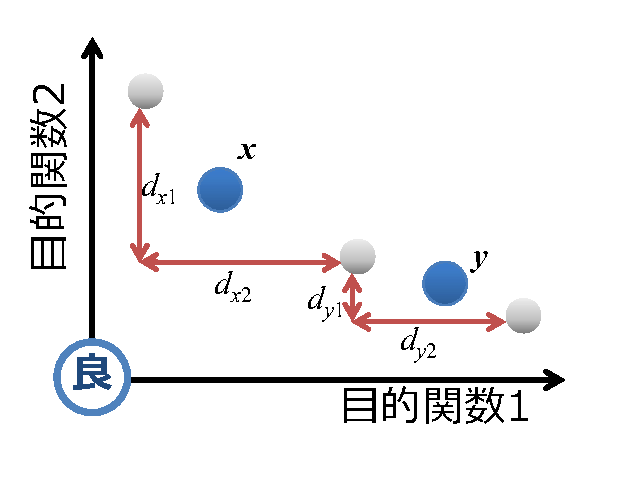
\includegraphics[width=0.5\textwidth,keepaspectratio=true]{fig/theory_crowding_distance.eps}
    \end{center}
    \caption{混雑度の概念図}
    \label{fig::theory_crowding_distance}
\end{figure}

\subsection{OMOPSO\cite{Sierra05}}\label{subsec::OMOPSO}
PSOを用いた多目的最適化手法にMOPSO(Multi-objective Particle Swarm Optimization)がある.OMOPSOは,通常のMOPSOに加え,リーダー粒子群と$\epsilon$-アーカイブという2つの解集合のアーカイブと突然変異操作を導入することにより多目的最適化における探索性能の改善を図ったアルゴリズムである.OMOPSOのアルゴリズムの流れを\figref{fig::theory_omopso}に示す.OMOPSOは,NSGA-IIと同様に解集合(=粒子群)$\mathcal{P}$を非支配ソートと混雑距離でランキングしリーダー粒子群$\mathcal{L}$を抽出する.リーダーを用いて粒子群を飛翔する.その後,粒子群を$\mathcal{Q}, \mathcal{R}, \mathcal{S}$に3分割し,粒子群$\mathcal{Q}$には一様突然変異,粒子群$\mathcal{R}$には非一様突然変異操作を加え,粒子群$\mathcal{S}$には何もしない.粒子群$\mathcal{Q}, \mathcal{R}, \mathcal{S}$を結合して次世代の粒子群$\mathcal{P}$とする.リーダー粒子群と$\epsilon$-アーカイブの和集合$\mathcal{L} \cup \mathcal{E}$の中で$\epsilon$優越する非劣解を$\epsilon$-アーカイブに格納し,最終世代の$\epsilon$-アーカイブ$\mathcal{E}$を非劣解集合として出力する.
OMOPSOの淘汰の手法は,NSGA-IIのように個体群(粒子群)の中から劣解を削除するような手法ではなく,リーダー粒子群と$\epsilon$-アーカイブという2つのアーカイブに良好な解を抽出する手法であるため,必ずしも探索個体群の中に良好な解が残っているとは限らず劣解や制約違反の解が残り続ける場合がある.OMOPSOでは,劣解も含む探索粒子群とリーダー粒子による飛翔をもとに新たな解を探索することと,アーカイブにはこれまでの探索で獲得したすべての$\epsilon$優越する非劣解を格納することで合理的な解を多数獲得できることが特徴である.
\begin{figure}[ht]
    \begin{center}
        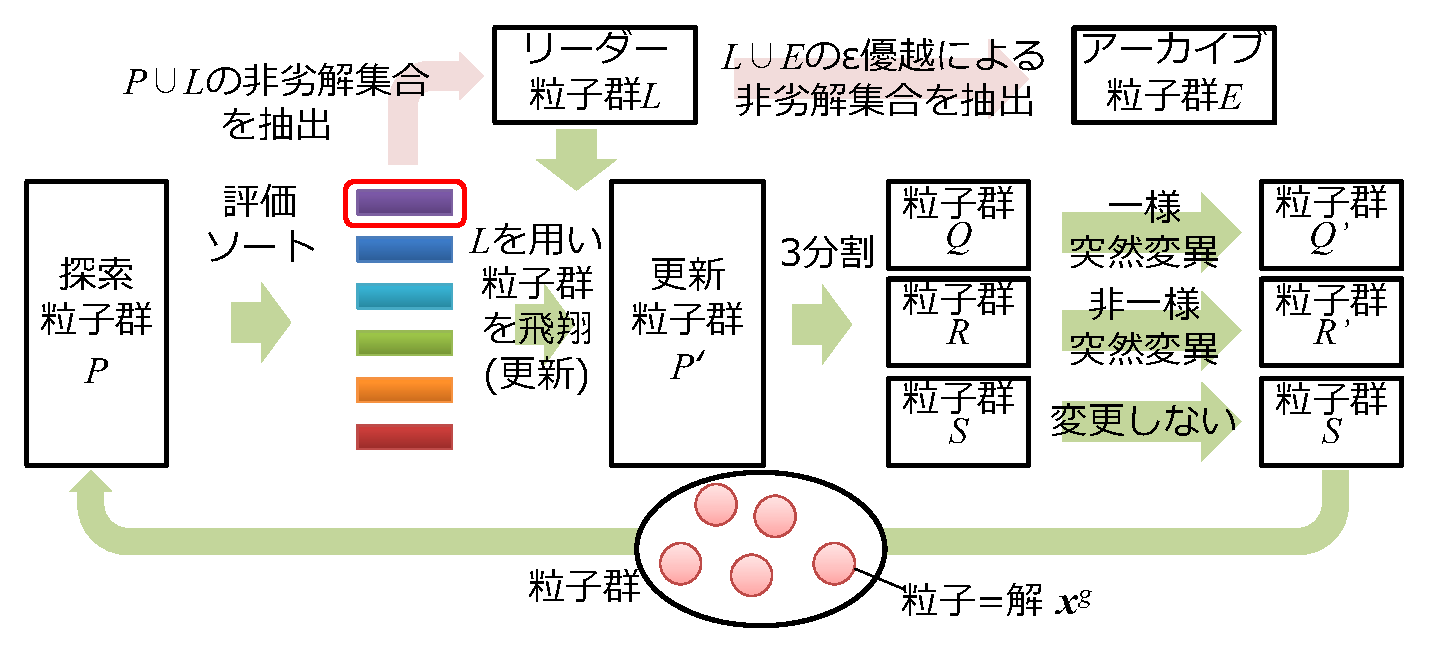
\includegraphics[width=1.0\textwidth,keepaspectratio=true]{fig/theory_omopso.eps}
    \end{center}
    \caption{OMOPSOのアルゴリズムのフロー}
    \label{fig::theory_omopso}
\end{figure}

\subsubsection{$\epsilon$-アーカイブ}
OMOPSOでは$\epsilon$-アーカイブと呼ばれる解集合のアーカイブを持つ.このアーカイブは,探索した解集合のうち,$\epsilon$優越するランク1の解を全て格納する,サイズ制限のないアーカイブである.$\epsilon$優越($\epsilon$-dominance)とは,通常の優越操作に対し,$\epsilon$だけ優越判定範囲を拡大したものである.$\epsilon$-アーカイブによる優越範囲と通常の優越範囲の例を\figref{fig::theory_epsilon_dominance}に示す.\figref{fig::theory_epsilon_dominance}の例では,解$\vec{x}$に対して$\vec{y}$は本来は優越されない位置にいるが,$\epsilon$優越の範囲には含まれるため,この解$\vec{y}$は$\vec{x}$に$\epsilon$優越される,と言う.このように優越範囲を拡張することで,あまりに近傍にある解や,ある1つの目的で大きく劣っている解を削除した合理的な解集合をアーカイブに残すことができる.

\begin{figure}[ht]
    \begin{center}
        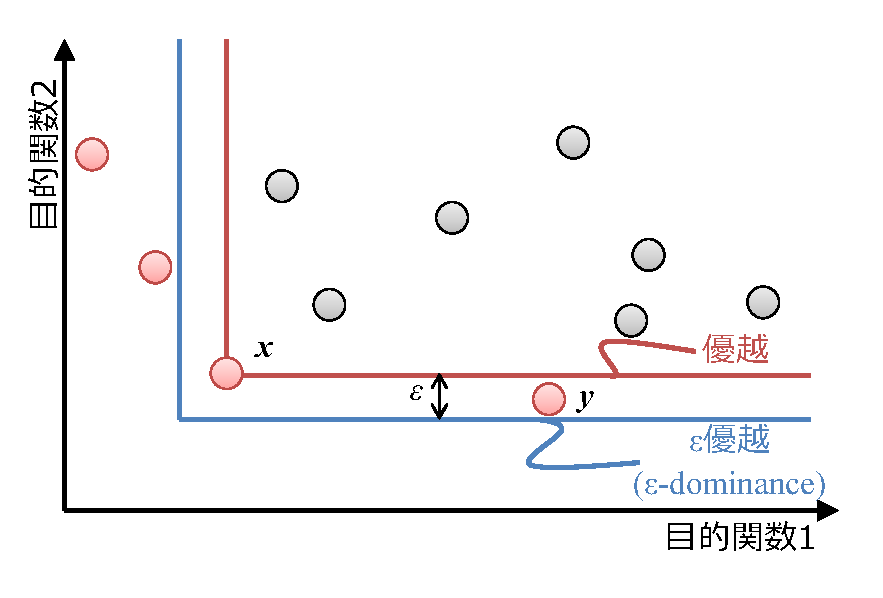
\includegraphics[width=0.7\textwidth,keepaspectratio=true]{fig/theory_epsilon_dominance.eps}
    \end{center}
    \caption{$\epsilon$優越の概念図}
    \label{fig::theory_epsilon_dominance}
\end{figure}

\subsubsection{OMOPSOのアルゴリズム}
OMOPSOの具体的なアルゴリズムを以下に示す.
\begin{description} \label{algo::OMOPSO}
    \setlength{\listparindent}{0pt}   %5. 最初のインデント
    \setlength{\itemsep}{0pt}      %2. ブロック間の余白    
    \item[Step 1:] サイズ$N^{\mathcal{P}}$のベース粒子群$\mathcal{P}$をランダムに生成し,世代数$g=0$にする.
    \item[Step 2:] 各粒子$\vec{x}^g \in \mathcal{P}$について,目的関数値と制約関数値を求め,パーソナルベストとする.
    \item[Step 3:] ベース粒子群$\mathcal{P}$における非劣粒子群をリーダー粒子群$\mathcal{L}$とアーカイブ粒子群$\mathcal{E}$にコピーする.
    \item[Step 4:] 各粒子$\vec{x}^g \in \mathcal{P}$の速度と位置を\Eqref{eq::theory_pso_velocity}, \eqref{eq::theory_pso_position}で更新する.ただし,$\vec{x}_{gbest}$は$\mathcal{L}$からバイナリトーナメント選択で選択された粒子の位置とする.更新した$\vec{x}^{g+1}$の各要素が,[$x^{min}, x^{max}$]の範囲を超過した場合,境界値まで引き戻し,さらに速度$\vec{v}^{g+1}$を$-1$倍する修復操作を施す.
    \item[Step 5:] $\mathcal{P}$を粒子群$\mathcal{Q}$,$\mathcal{R}$,$\mathcal{S}$へ均一に分割する.
    \item[Step 6:] 粒子群$\mathcal{R}$の各粒子に$[-0.25(x^{max}- x^{min}), 0.25(x^{max}- x^{min})]$の範囲の一様乱数値を加える一様突然変異,粒子群$\mathcal{S}$の各粒子に\Eqref{eq::theory_mutation_nonuni}による非一様突然変異を施し,粒子群$\mathcal{Q}$には何もしない.
    \item[Step 7:] 粒子群$\mathcal{Q}$, $\mathcal{R}$, $\mathcal{S}$を結合し,新たな粒子群$\mathcal{P}$ (=$\mathcal{Q}\cup\mathcal{R}\cup\mathcal{S}$)とする.
    \item[Step 8:] 粒子群$\mathcal{P}$の各粒子を評価し,目的関数値と制約関数値を求め,パーソナルベストを後述の制約支配する場合,パーソナルベストを更新する.
    \item[Step 9:] $\mathcal{P} \cup \mathcal{L}$の粒子群における非劣粒子群をリーダー粒子群$\mathcal{L}$にする.同様に,$\mathcal{L} \cup \mathcal{E}$の粒子群における非劣粒子群をアーカイブ粒子群$\mathcal{E}$にする.リーダー粒子群$\mathcal{L}$がサイズ$N^{\mathcal{L}}$を超過する場合,混雑距離の上位$N^{\mathcal{L}}$までを$\mathcal{L}$に残し,それ以外は$\mathcal{L}$から削除する.
    \item[Step 10:] 世代数$g$に1を加算し,総世代数$g_{max}$に達したとき,アーカイブ粒子群$\mathcal{E}$を最適化の結果として出力して終了する.そうでなければ{\bf Step 4}に戻る.
\end{description}



\subsection{制約条件の取り扱い\cite{Coello02, Harada07}}
進化計算のように多数の解集合を交叉と世代交代によってパレート最適解集合を探索する手法は,探索過程において実行不可能解を生成することがある.また,実行可能範囲が狭い問題や偏りのある問題では,初期解をランダムに生成しても実行可能解は生成されず,探索初期には実行可能解を探索しなければならない場合がある.そこで,探索中の制約の取り扱い方法がいくつか考案されている.ここでは標準的に用いられる手法と,本研究で採用する制約優越について述べる.

\subsubsection{デス・ペナルティ法}
デス・ペナルティ法(Death Penalty)は,探索中の解集合のうち実行不可能解を削除する方法である.これによって探索によって得られた実行可能解を残し,実行可能解のみから交叉することによって新たな実行可能解の探索を促進する.一方で,上述のように実行可能範囲が狭い問題では,新たに生成される子個体の多くが削除されてしまい,探索が進まないことがある.

\subsubsection{ペナルティ法}
解が制約を満たさない場合に,制約違反の度合い(制約違反量, Constraint Violation Degree)を計算する関数(ペナルティ関数)$v(\vec{x})$を定義し,ペナルティ関数値を目的関数値に足し合わせて,それを最小化(もしくは最大化)することによって,実行可能解と同時に目的関数値の良い解を探索する手法である.ペナルティ法で用いられる制約なし多目的最適化問題は,以下のように定義される.

\begin{align}
    \mbox{Minimize/Maximize} \quad \vec{f}(\vec{x}) + v(\vec{x})
\end{align}

本手法に対しては,ペナルティ関数のレンジを目的関数に合わせて調整するなど適切なペナルティ関数を定義しなければならないこと,目的関数に対応しない制約が複数存在する場合に適用が困難なことが課題として挙げられている.

\subsubsection{制約の目的関数化}
制約違反量を,追加目的関数とした多目的最適化問題を解くことにより,実行可能でかつ目的関数の良好な解を探索する手法である.制約を目的として追加した新たな目的関数は,以下のように定義される.

\begin{align}
    \mbox{Minimize/Maximize} \quad \vec{f}(\vec{x}) = \{f_1(\vec{x}), \cdots,f_m(\vec{x}), g_1(\vec{x}), \cdots, g_p(\vec{x})\}
\end{align}
この手法では,制約条件も目的関数とすることで,制約を満たしながら良好な解を探索できる,ある程度制約違反を許容しつつ目的関数値の良い解も探索できる,という利点がある.そのため,制約が,必ず満たさなければならない強い制約ではなく,ある程度の違反が許容される弱い制約である場合や,制約条件の範囲が未確定である場合に有効である.一方で,本手法をとると問題によっては最終世代の解集合に実行不可能な解が残ってしまうことになる.そのため,最終世代のパレート解集合のうち実行可能解は限定されてしまい,全ての個体を有効に活用できない場合がある.

\subsubsection{制約優越法\cite{Deb02}}
制約優越法は,ペナルティ法と同様にペナルティ関数$v(\vec{x})$を定義する.ある2つの解の優越を比較をする際に,いずれも制約を満たすかどうか,制約を満たす場合は目的関数値で,制約を満たさない場合は制約違反量で優越判定をすることで,制約を満たし,かつ目的関数値が良好である解の探索を促進する手法である.2つの解$\vec{x}$, $\vec{y}$について,$\vec{x}$が$\vec{y}$に制約優越する(または制約支配する)という場合は以下のいずれかを満たすことを指す.

\begin{itemize}
    \item $\vec{x}$が実行可能であり,$\vec{y}$が実行不可能である
    \item $\vec{x}$と$\vec{y}$両方が実行不可能で,$\vec{x}$の制約違反量$v(\vec{x})$が$\vec{y}$の制約違反量$v(\vec{y})$に対して小さい$(v(\vec{x})<v(\vec{y}))$
    \item $\vec{x}$と$\vec{y}$両方が実行可能で,$\vec{x}$の目的関数が$\vec{y}$を優越している
\end{itemize}

制約優越では,ペナルティ法とは異なりペナルティ関数のレンジを目的関数に合わせる必要がないこと,目的関数の数に依存せずペナルティ関数を定義できることから,目的関数に関わらない種々の制約を持つ実問題においても容易に制約を扱うことができる.そこで,本研究では,制約優越を採用することで制約条件を取り扱う.

\chapter{数理モデル最適化}
\label{chap::math}

\hspace{1zw}本章では,オフィスビルの一室の空調設定スケジュールを最適化するため,数理モデルを用いる手段について述べる.
\section{概要}

\subsection{システム構成}
\hspace{1zw}数理モデルによる最適化システムの構成を\figref{fig::math_system}に示す.本システムは,最適化部と評価部からなる.評価部は,最適化部から空調設定温度スケジュール(解)を受け取り,数理モデルに基づいて室内快適性とエネルギー消費量を算出して最適化部に渡す.最適化部は,その結果に基づいて解を比較し,新しい解の生成を繰り返す.本システムの出力は,最適化された空調設定スケジュール集合である.

\begin{figure*}[t]
  \begin{center}
    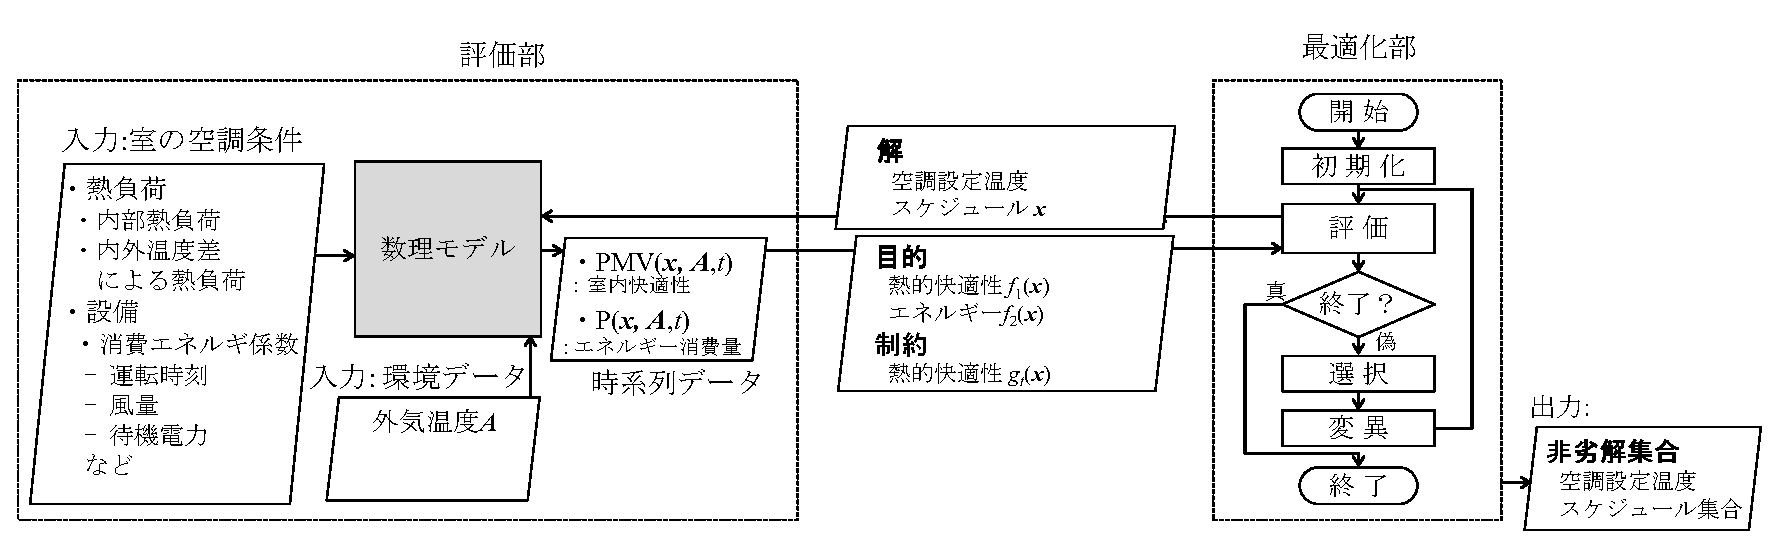
\includegraphics[width=1.1\linewidth]{fig/math_system.eps}
  \end{center}
  \vspace{-0.5cm}
  \caption{数理モデル最適化システム}
  \label{fig::math_system}
\end{figure*}


\subsection{最適化対象のオフィス}
本章では,\figref{fig::math_office_room}に示すオフィスの一室を対象にする.本空調環境は,東京都内の8階建てビルの5階に位置する窓のない部屋で,広さは37.6 [m$^2$]である.この部屋にはビル用マルチエアコンが設置されている.エアコンは,独立した室外機と冷媒系統を用い,冷暖房能力7.1 [kW]の4方向吹出口を持つ室内機を2台設置している.部屋の広さと空調機の能力を\tabref{tab::math_office_spec}に示す.

\begin{figure}[t]
  \begin{center}
    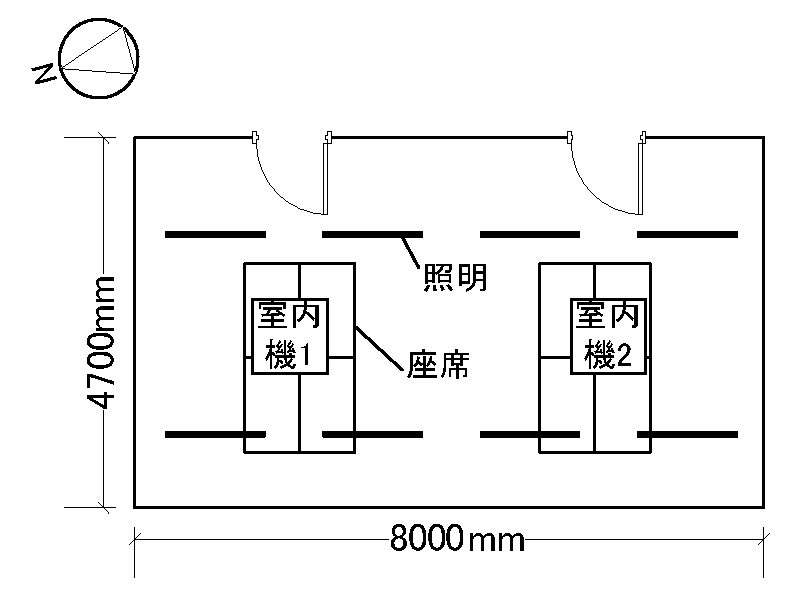
\includegraphics[width=0.6\linewidth]{fig/math_office_room.eps}
  \end{center}
  \vspace{-0.5cm}
  \caption{オフィスビルの1室}
  \label{fig::math_office_room}
\end{figure}

\begin{table}[b]
  \caption{空調環境諸元}
  \label{tab::math_office_spec}
  \centering
  \begin{tabular}{c|cccc}
    \hline
    項目           & 値               \\
    \hline    \hline
    面積[m$^2$]    & 37.6             \\
    室外機能力[kW] & 14               \\
    室内機能力[kW] & 7.1$ \times $2台 \\
    \hline
  \end{tabular}
\end{table}

\section{数理モデル最適化における解評価}
本節では,上述のオフィスの部屋に対して適用する空調設定スケジュールの評価を行うために目的関数を定義し,空調設定スケジュール最適化問題を多目的最適化問題として定式化する.

\subsection{設計変数}
従来の空調システムは,ビル管理者が,季節または月・日ごとに,これまでのエネルギー消費量の傾向と室内環境の履歴から,当日の設定温度を決定する.空調設定温度スケジュール最適化では空調の設定温度を分割時間間隔$T_s$毎に変更することとし,1日の設定温度スケジュール$t_{set}(\vec{x},t) (t \in \mathcal{T}_{set})$を最適化する.本章では,$T_s=0.5$[hour]とし設定可能時刻集合を$\mathcal{T}_{set}=\{8:00, 9:30,\dots, 22:00\}$とする.
設定温度スケジュール$t_{set}(\vec{x},t)$を設計変数ベクトル$\vec{x}$で表すためには,以下のように,設計変数ベクトルの各要素$x_t$を設定可能時刻$t$における設定温度$t_{set}(\vec{x},t)$とする方法が考えられる.
\begin{equation}
  t_{set}(\vec{x},t) = x_t ~~~~~~~(t \in \mathcal{T}_{set})
  \label{eq::math_variable}
\end{equation}

しかしながら,この手法では後述の制約条件\Eqref{eq::math_constraint_tset_diff}を満たさないスケジュールが多く探索空間が膨大となり,良好な解の探索に時間がかかる.そこで,本研究では以下の通り,設計変数ベクトルの1つ目の要素は空調設定温度スケジュールの初期温度,設計変数ベクトルの2つ目以降の要素は空調設定温度スケジュールの前の時刻との差を示すものとする.

\begin{align}
  t_{set}(\vec{x},t) & =
  \begin{cases}
    x_t ~~~~~~~~~~~~~~                          & (t=8:00)                 \\
    t_{set}(\vec{x},t-T_s) + x_t ~~~~~~~~~~~~~~ & (t=8:30, 9:00,...,22:00) \\
  \end{cases}
  \label{eq::math_variable_diff}
\end{align}

\subsection{第一目的関数}
第一目的は,室内快適性の向上である.オフィスワーカーの快適性の評価が可能な快適性指標には様々なものがあるが,ここでは,PMV (Predicted Mean Vote)を用いる.PMVは,国際標準化機構(International Standardization Organization, ISO)によって標準化された室内の平均的な温冷感の指標である\cite{ISO05}.PMVは,室内の平均的な温度,湿度,風速,平均放射温度の4つの環境計測値およびオフィスワーカーの代謝量,着衣量の2つの人に依存する物理量から,温冷感を$-3$(寒い)から$+3$(暑い)までの7段階で算出する.PMV=0が最も快適な環境である.PMVの絶対値が大きいほど,不快な環境になる.第一目的関数を次式で定義する.

\begin{equation}
  \mbox{Minimize} \quad f_1(\vec{x},\mathcal{A}) = \frac{1}{|\mathcal{T}_1|} \sum_{t\in \mathcal{T}_1} | PMV(\vec{x},\mathcal{A},t) |
  \label{eq::math_objective1}
\end{equation}

ここで,$\mathcal{T}_1$は室内快適性を計測する時刻集合であり,設計変数ベクトルと同様30分間隔で$\mathcal{T}_1=\{7:00, 7:30,\dots, 21:30, 22:00\}$とする.
$PMV(\vec{x},\mathcal{A},t)$は,時刻$t$におけるPMVであり,外気温の影響を受けるため,30分ごとの外気温集合$\mathcal{A}=\{a_{00:00},a_{00:30},\dotsc,a_{23:30},a_{24:00}\}$を入力する.

本章では,$PMV(\vec{x},\mathcal{A},t)$の算出にISOが定義する以下の数理モデルを採用した.
\begin{align}
   & PMV(\vec{x},\mathcal{A},t) = (0.303\mathrm{e}^{-0.036M}+0.028)\cdot \nonumber \\
   & ~~~~~~~~~ H(T_a(\vec{x},t), R_h, V_a(t), T_r(\vec{x},t), M, I_{cl})
  \label{eq::math_pmv}
\end{align}
ここで,$H(T_a, R_h, V_a, T_r, M, I_{cl})$は人体の発熱量を示す関数である.また,$T_a(\vec{x},t)$は温度[$^o$C],$R_h$は湿度$[\%]$, $V_a(t)$は風速[m/s],$T_r(\vec{x},t)$は平均放射温度[$^o$C],$M$は代謝量[met],$I_{cl}$は着衣量[clo]である.本来,環境計測値は,空調設定および外気温$\mathcal{A}$や外気導入量等によって変動し,代謝量・着衣量は人によって異なるが,ここでは単純化のために,下記の式のように,温度および平均放射温度が空調設定スケジュール$\vec{x}$のみによって変動するものとし,他の湿度,風速,着衣量,代謝量は固定値か季節で一定の値とした.
\begin{align}
  T_a(\vec{x},t) & =
  \begin{cases}
    t_{set}(\vec{x},t) + 1.0 (夏季) & \\
    t_{set}(\vec{x},t) - 1.0 (冬季) & \\
  \end{cases}
  \label{eq::math_temperature}
\end{align}
\begin{align}
  T_r(\vec{x},t) & =
  \begin{cases}
    T_a(\vec{x}, t) + 0.2 (夏季) & \\
    T_a(\vec{x}, t) - 0.2 (冬季) & \\
  \end{cases}
  \label{eq::math_radiation}
\end{align}
\begin{align}
  R_h & =
  \begin{cases}
    55 (夏季) & \\
    45 (冬季) & \\
  \end{cases}
  \label{eq::math_humidity}
\end{align}
\begin{align}
  V_a & =V_{in}-1.0
  \label{eq::math_airvolume}
\end{align}
\begin{align}
  I_{cl} & =
  \begin{cases}
    0.6 (夏季) & \\
    0.8 (冬季) & \\
  \end{cases}
  \label{eq::math_cloth}
\end{align}
\begin{align}
  M & =1.1
  \label{eq::math_metabolic}
\end{align}
ただし,$V_{in}$は空調機の風量設定値[m$^3$/min]である.

\subsection{第二目的関数}
第二目的は,エネルギー消費量の最小化である.設計変数$\vec{x}$のエネルギー消費量に関する目的関数を次式で表す.
\begin{equation}
  \mbox{Minimize} \quad f_2(\vec{x},\mathcal{A}) = \sum_{t\in \mathcal{T}_2} P(\vec{x},\mathcal{A},t)
  \label{eq::math_objective2}
\end{equation}
ここで,$\mathcal{T}_2$はエネルギー消費量を計測する時刻集合であり,$\mathcal{T}_2=\{0:00, 0:30,\dots, 24:00\}$とする.$P(\vec{x},\mathcal{A},t)$は,時刻$t$のエネルギー消費量[W]であり,外気温集合$\mathcal{A}$の影響を受ける.

本章では,エネルギー消費量$P(\vec{x},\mathcal{A},t)$の算出に数理モデルを用いる.
\figref{fig::math_office_room}の空調システムのエネルギー消費量$P(\vec{x},\mathcal{A},t)$を,空調機にかかる熱負荷を用いて算出する\cite{Kuki12}.熱負荷は,空調機が部屋の空間に対して供給/除去する熱量である.熱負荷は,本来,建物の熱貫流や日射,換気,蓄熱,空気の移動などを考慮して算出するが,ここでは,簡易的に室内に発生する内部熱負荷と,室外との間で発生する外部熱負荷を用いて次式で算出する.
\begin{align}
  Q_{in}(t)                      & = Q_{people}(t) + Q_{light}(t) + Q_{oa}(t)
  \label{eq::math_heatload_in}                                                \\
  Q_{out}(\vec{x},\mathcal{A},t) & = (a_t - t_{set}(\vec{x},t)) Q_{temp}
  \label{eq::math_heatload_out}
\end{align}
\vspace{-0.8cm}
\begin{align}
  Q(\vec{x},\mathcal{A},t) & =
  \begin{cases}
    Q_{out}(\vec{x},\mathcal{A},t) + Q_{in}(t)~(冷房時) & \\
    Q_{out}(\vec{x},\mathcal{A},t) - Q_{in}(t)~(暖房時) & \\
  \end{cases}
  \label{eq::math_heatload}
\end{align}
ここで,$Q(\vec{x},\mathcal{A},t) $は総熱負荷,$Q_{people}(t)$は人体の熱負荷[W],$Q_{light}(t)$は照明の熱負荷[W],$Q_{oa}$は機器熱負荷[W],$Q_{temp}$は室内外温度差による熱負荷基準値[W/$^o$C]である.
空調システムが上述の熱負荷を処理するために必要とするエネルギー量$P$は,外気温度や空調機の動作条件によって変動するが,ここでは熱負荷に比例するものと仮定し次式で算出する.
\begin{align}
  P(\vec{x},\mathcal{A},t) & = P_zQ(\vec{x},\mathcal{A},t)+P_{fin}V_{fin}+P_{out}
  \label{eq::math_energy}
\end{align}
ここで,$P_z$は熱負荷とエネルギー消費量との比例係数,$P_{fin}$は室内機の風量$V_{fin}$と室内機ファンのエネルギー消費量の比例係数[$W \cdot$ min / m$^3$],$P_{out}$は室外機の待機電力[W]である.

\subsection{制約条件}
\subsubsection{快適性に関する制約}
快適性に関する制約条件を設ける.ISOでは,室内の不快な環境を避けるため,不満足者率が10\%以下となるようPMV値を$-0.5$から$+0.5$の範囲内に保つことを推奨している.そこで,次式で示すPMV値の絶対値の上限値を設定する.
\begin{equation}
  \mbox{Subject\ to} ~~~g_t(\vec{x})=|PMV(\vec{x},\mathcal{A}, t) |  \leq 0.5\quad(t \in \mathcal{T}_1)
  \label{eq::math_constraint_pmv}
\end{equation}
全ての時刻$t$に対して上記の制約条件を満たす解を実行可能解,ひとつでも満たさない時刻がある解を実行不可能解とする.制約総違反量$v(\vec{x})$を次式で表す.
\begin{equation}
  v(\vec{x}) = \sum_{t\in \mathcal{T}_1}  \max_{}{\{0,~g_t(\vec{x})-0.5\}}
  \label{eq::math_constraint_violation_pmv}
\end{equation}

\subsubsection{空調設定温度に関する制約}
空調設定温度は,設定できる値と範囲が空調機の機種によって制限される.本章では,設定可能な値は最大値・最小値の範囲内とする.また,設定温度は0.5[$^o$C]刻みで設定できるものとする.さらに,設定温度の大きく変更することによる突発的なエネルギー消費の増加を避けるため,隣接した時間帯では設定温度の変更量を$\pm1$[$^o$C]以内に制限する.これらを制約条件とし,以下の\Eqref{eq::math_constraint_tset_minmax}~\eqref{eq::math_constraint_tset_diff}で表す.
\begin{eqnarray}
  T_{min} \leq t_{set}(\vec{x},t) & \leq T_{max}
  \label{eq::math_constraint_tset_minmax} \\
  2 t_{set}(\vec{x},t) & \in \bf{Z}
  \label{eq::math_constraint_tset_int} \\
  |t_{set}(\vec{x},t) - t_{set}(\vec{x},t-T_{s})| & \leq 1
  \label{eq::math_constraint_tset_diff}
\end{eqnarray}
ここで,$T_{min}$,$T_{max}$はそれぞれ設定温度として設定可能な最小値,最大値である.また,$\bf{Z}$は整数の全体からなる集合である.

これらの設定温度に関する制約のうち\Eqref{eq::math_constraint_tset_int}および\Eqref{eq::math_constraint_tset_diff}は,設計変数が実数で設定された場合に,制約を満たすことが難しく,実行可能範囲が狭くなってしまい進化計算による探索を遅らせる原因になる.そこで,以下2つによりこれらの制約の範囲が解探索空間となるような工夫を行う.
\begin{enumerate}
  \item 設計変数ベクトルの各要素$x_t$が設定温度スケジュールの各時刻の設定温度$t_{set}(\vec{x},t)$を直接表す\Eqref{eq::math_variable}の形態ではなく,\Eqref{eq::math_variable_diff}のように設計変数ベクトルの1つ目の要素は空調設定温度スケジュールの初期温度,設計変数ベクトルの2つ目以降の要素は空調設定温度スケジュールの次の時刻との差を示すものとする.差を\Eqref{eq::math_constraint_tset_diff}を満たすよう$\pm$1[$^o$C]とすることで,制約範囲内の解のみを探索することにする.
  \item 設計変数から得られる空調設定スケジュールは実数の値であるが,これを最も近い\Eqref{eq::math_constraint_tset_int}を満たす値に丸めることとする.
\end{enumerate}

\section{実験内容}\label{sec::math_setting}
空調設定スケジュール最適化のために,前節で定義した空調設定スケジュール最適化問題に対して\subsecref{subsec::OMOPSO}で述べたOMOPSOアルゴリズムを適用して,パレート解集合を探索する.OMOPSOを採用した理由として以下が挙げられる.

\begin{itemize}
  \item OMOPSOはいくつかのベンチマークで,多目的最適化手法として代表的なNSGA-IIより良好な性能を持つこと\cite{Godinez10}
  \item 空調設定スケジュール最適化問題に類似した照明制御の問題において良好な性能を持つこと\cite{Ohta13}
  \item パラメータが乱数化されていて細かな調整が不要であること
  \item 良好な解を無制限に保存する仕組み(アーカイブ)を持ち,他の固定サイズアーカイブを持つ手法と比べてより多数の有用な解を意思決定者に提示できること
\end{itemize}

空調環境の条件は,冬季の晴れの日を想定して\tabref{tab::math_param_condition}のように定める.外気温$T_{out}$及び人体熱負荷$Q_{people}$・照明熱負荷$Q_{light}$・機器熱負荷$Q_{oa}$は時間帯によって変動する.外気温の1日の推移を\figref{fig::math_outside_temp}に,人体熱負荷$Q_{people}$,照明熱負荷$Q_{light}$,機器熱負荷$Q_{oa}$を合わせた内部熱負荷$Q_{in}$の1日の推移を\figref{fig::math_internal_heatload}に示す.対象オフィスでは12時~13時の間は昼休みであり,オフィスの在室者が減り内部熱負荷が減少する.そのため,12時~13時の時間帯は\Eqref{eq::math_constraint_pmv}のPMV値に関する制約を満たさなくても良いものとする.

\begin{figure}[ht]
  \begin{center}
    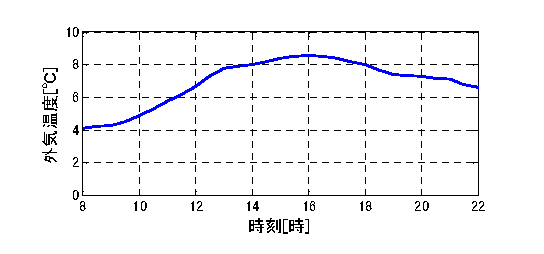
\includegraphics[width=85mm]{fig/math_outside_temp.eps}
  \end{center}
  \caption{外気温$T_{out}$の時間推移}
  \label{fig::math_outside_temp}
\end{figure}
\begin{figure}[ht]
  \begin{center}
    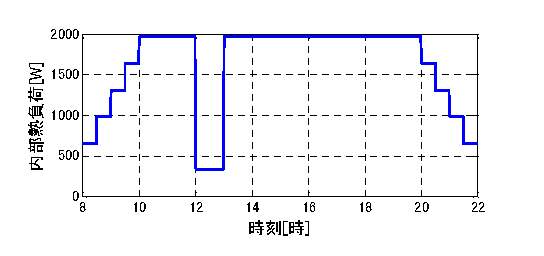
\includegraphics[width=85mm]{fig/math_internal_heatload.eps}
  \end{center}
  \caption{内部熱負荷$Q_{in}$の時間推移}
  \label{fig::math_internal_heatload}
\end{figure}

\begin{table}[htbp]
  {\small
    \begin{center}
      \caption{空調環境条件}
      \begin{tabular}{c|cccc}
        \hline
        項目                                      & 値                                           \\
        \hline    \hline
        外気温度$T_{out}$[$^o$C]                   & \figref{fig::math_outside_temp}に示す        \\
        人体熱負荷$Q_{people}$[kW]                & 3つを合計した                                \\
        照明熱負荷$Q_{light}$[kW]                 & 内部熱負荷$Q_{in}$                           \\
        機器熱負荷$Q_{oa}$[kW]                    & を\figref{fig::math_internal_heatload}に示す \\
        温度差による熱負荷基準値$Q_{temp}$[W/$^o$C] & 400                                          \\
        熱負荷-エネルギー消費量比例係数$P_z$[-]   & 0.25                                         \\
        風量-エネルギー消費量比例係数$P_{fin}$[-] & 10                                           \\
        室外機待機電力$P_{out}$[W]                & 50                                           \\
        設定温度最小値$T_{min}$[$^o$C]             & 17                                           \\
        設定温度最大値$T_{max}$[$^o$C]              & 28                                           \\
        室内機吹出風量$V_{in}$[$m^3$/$min$]           & 12                                           \\
        運転開始時刻$T_{start}$                   & 08:00                                        \\
        運転終了時刻$T_{end}$                     & 22:00                                        \\
        分割時間間隔$T_s$[hour]                   & 0.5                                          \\
        時間分割数$N_t$                           & 29                                           \\
        \hline
      \end{tabular}
      \label{tab::math_param_condition}
    \end{center}
  }
\end{table}

OMOPSOアルゴリズムのパラメータは\tabref{tab::math_param_algo}のように定める.ここで,重み$w, c_1, c_2$は文献\cite{Sierra05}の推奨値を用いた.また,$\epsilon$優越する範囲を調整する係数$\epsilon$は,値が探索結果に大きく影響する.そこで,本問題に適切な$\epsilon$の値を検討するため,$\epsilon=0, 0.0075, 0.05$と変更して複数回探索を試行した.
本章では,数理モデルおよびOMOPSOアルゴリズムをプログラミング言語Javaで実装した.計算機環境には,一般的なビル管理システムの計算能力を想定して,Windows 7 (64ビット),Intel Core i7-2600S (2.8GHz)およびRAM 8GBのPCを用いた.

\begin{table}[t]
  {\small
    \begin{center}
      \caption{OMOPSOのパラメータ}
      \label{tab::math_param_algo}
      \begin{tabular}{c|cccc}
        \hline
        パラメータ                             & 方法 / 値              \\
        \hline \hline
        ベース粒子群サイズ $N^{\mathcal{P}}$   & 100                    \\
        リーダー粒子群サイズ $N^{\mathcal{L}}$ & 100                    \\
        アーカイブ粒子群サイズ                 & 制限なし               \\
        総世代数 $g_{max}$                     & 10000                  \\
        変数帳 $n$                             & 29                     \\
        突然変異率 $p_m$                       & $1/n$                  \\
        重み $w$                               & [$0.1, 0.5$)の一様乱数 \\
        重み $c_1, c_2$                        & [$1.5, 2.0$)の一様乱数 \\
        非一様突然変異の係数 $b$               & 5 \cite{Esquivel03}    \\
        $\epsilon$優越の係数$\epsilon$         & 0, 0.0075, 0.05        \\
        \hline
      \end{tabular}
    \end{center}
  }
\end{table}

\section{実験結果と考察}
\subsection{実験結果}

数理モデル最適化によって得られた空調設定スケジュールの集合を\figref{fig::math_result_pareto_eps}に$\epsilon$の値ごとに青点で示す.
それぞれの図について,横軸が室内快適性$f_1$, 縦軸がエネルギー消費量$f_2$であり,どちらも小さいほど良好なスケジュールであることを示す.数理モデル最適化によって,$\epsilon=0$では76個,$\epsilon=0.0075$では56個,$\epsilon=0.05$では29個のスケジュールが獲得できた.数理モデル最適化によって得られたスケジュール集合は,室内快適性とエネルギー消費量のトレードオフを示すことがわかる.また,スケジュール集合は制約\Eqref{eq::math_constraint_pmv}を満たす平均$|$PMV$|$の範囲0~0.5のうち広い範囲の解を含んでいる.ただし,制約範囲の境界付近である$|$PMV$|\leq 0.1$と$|$PMV$|\geq 0.4$ の範囲では獲得された解の数が少ない.さらに,$\epsilon$の値が大きくなるごとに境界付近で良い解を探索できなくなり,解の分布が均等でなくなっている.

\begin{figure*}[htbp]
  \begin{center}
    \begin{minipage}{0.6\textwidth}
      \begin{center}
        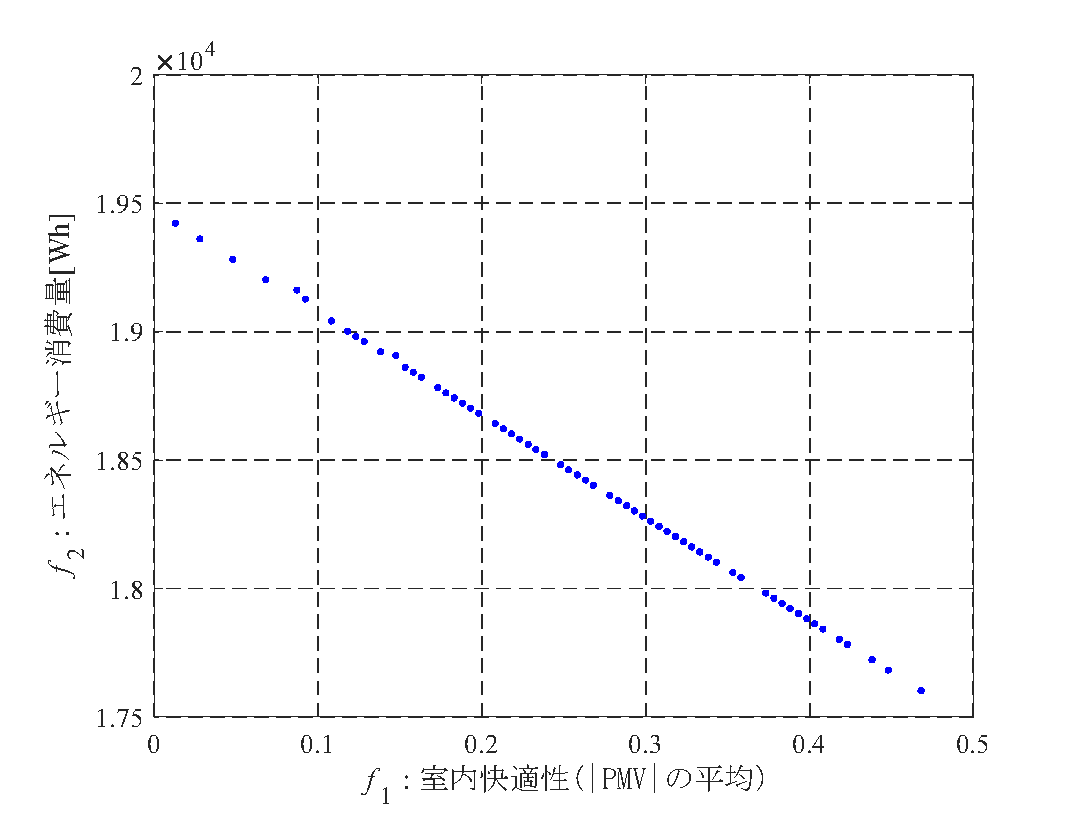
\includegraphics[width=1.0\textwidth,keepaspectratio=true]{fig/math_result_pareto_eps1.eps}\\\vspace{-0.3cm}{{(a) $\epsilon=0$}}
      \end{center}
    \end{minipage}
    \begin{minipage}{0.6\textwidth}
      \begin{center}
        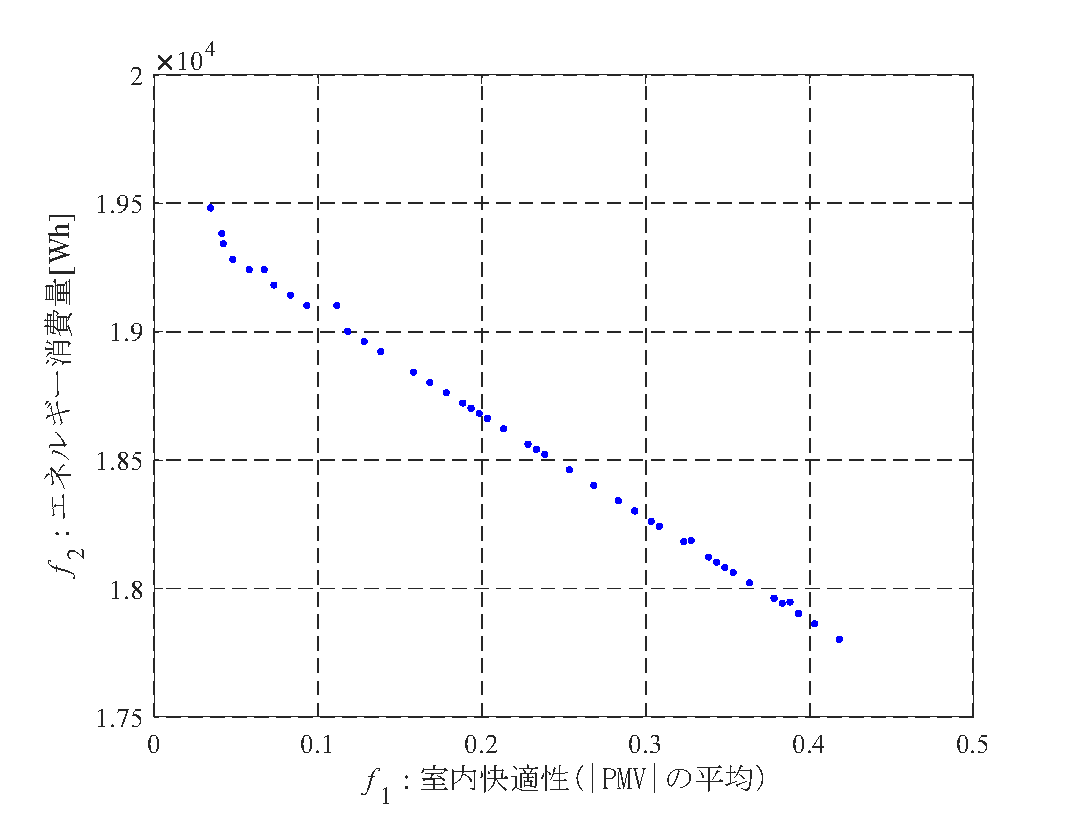
\includegraphics[width=1.0\textwidth,keepaspectratio=true]{fig/math_result_pareto_eps2.eps}\\\vspace{-0.3cm}{{(b) $\epsilon=0.0075$}}
      \end{center}
    \end{minipage}
    \begin{minipage}{0.6\textwidth}
      \begin{center}
        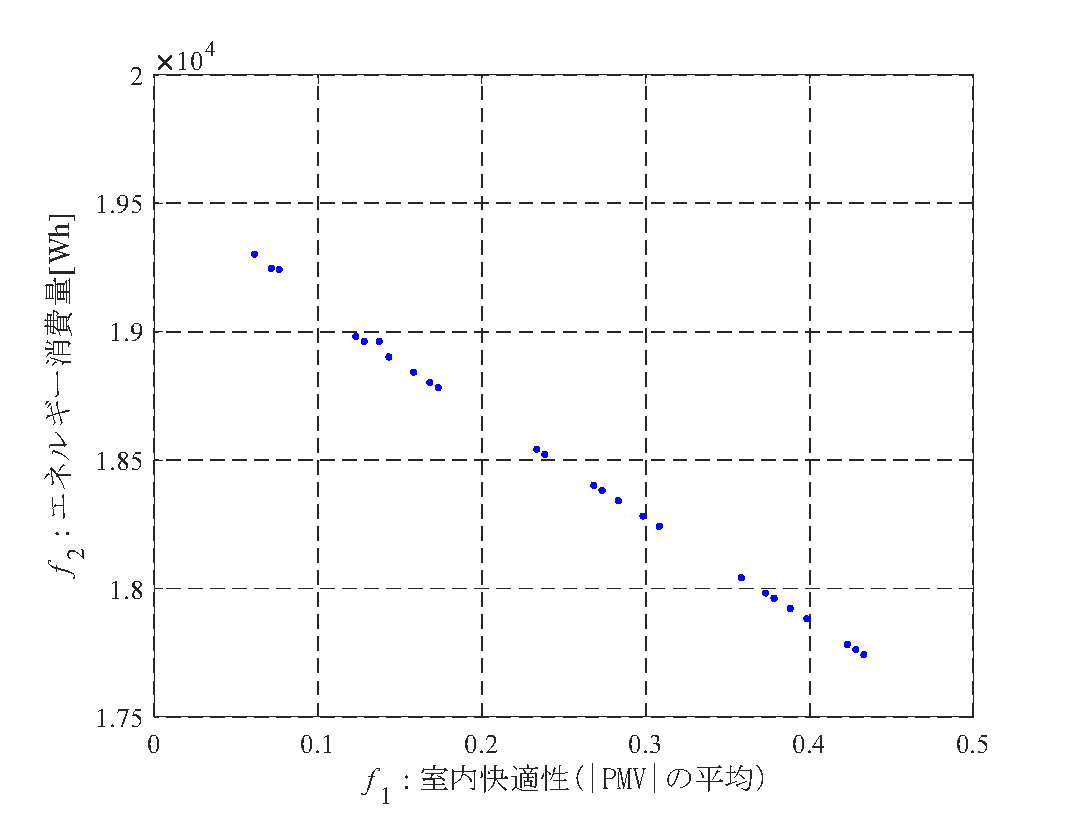
\includegraphics[width=1.0\textwidth,keepaspectratio=true]{fig/math_result_pareto_eps3.eps}\\\vspace{-0.3cm}{{(c) $\epsilon=0.05$}}
      \end{center}
    \end{minipage}
  \end{center}
  \vspace{2mm}
  \caption{$\epsilon$を変更した場合の数理モデル最適化の結果}
  \label{fig::math_result_pareto_eps}
\end{figure*}

\begin{comment}
最も広い範囲を均等に探索できた$\epsilon=0$のパレート解に対し,比較のために従来法である設定温度を終日一定値に設定した解を同一目的関数空間上に赤のアスタリスクで図示したものを\figref{fig::math_result_pareto}に示す.数理モデル最適化は,設定温度を一定にする従来法のスケジュールをパレート支配するスケジュールを獲得しており,良好なスケジュールが得られたといえる.

\begin{figure}[htbp]
  \begin{center}
    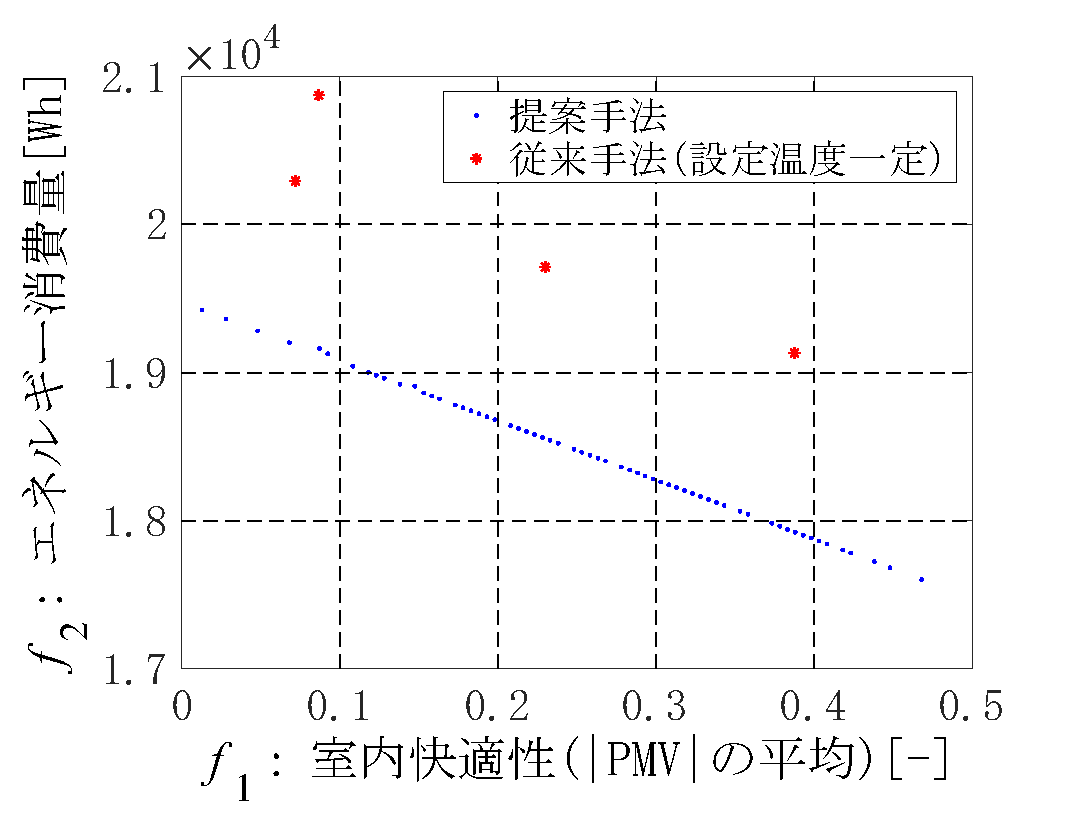
\includegraphics[width=0.7\linewidth]{fig/math_result_pareto.eps}
  \end{center}
  \caption{数理モデル最適化による解集合と設定温度一定解の比較}
  \label{fig::math_result_pareto}
\end{figure}
\end{comment}

最も広い範囲を均等に探索できた$\epsilon=0$の探索で得られたスケジュール集合のうち例として,室内快適性の目的関数値が最も小さい快適な解($f_1=0.0279$),最も値の大きい不快な解($f_1=0.463$),中間の解($f_1=0.233$)の設定温度スケジュールの例と,そのスケジュールで運転した際の快適性・エネルギー消費量の推移を\figref{fig::math_result_schedule}に示す.昼の時間帯を除き,すべての時間帯で\Eqref{eq::math_constraint_pmv}を満たすよう制御できていることがわかる.

\begin{figure}[htbp]
  \centering
  \subfigure{
    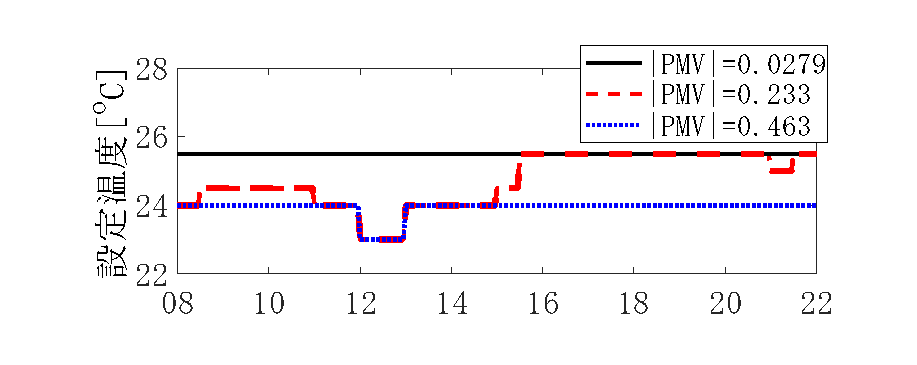
\includegraphics[width=0.6\textwidth,keepaspectratio=true]{fig/math_result_schedule_settemp.eps}
    \label{fig::math_result_schedule_settemp}
  }
  \subfigure{
    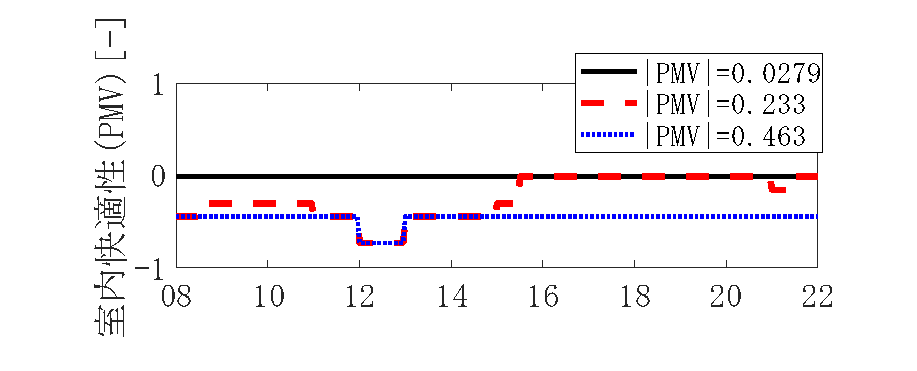
\includegraphics[width=0.6\textwidth,keepaspectratio=true]{fig/math_result_schedule_pmv.eps}
    \label{fig::math_result_schedule_pmv}
  }
  \subfigure{
    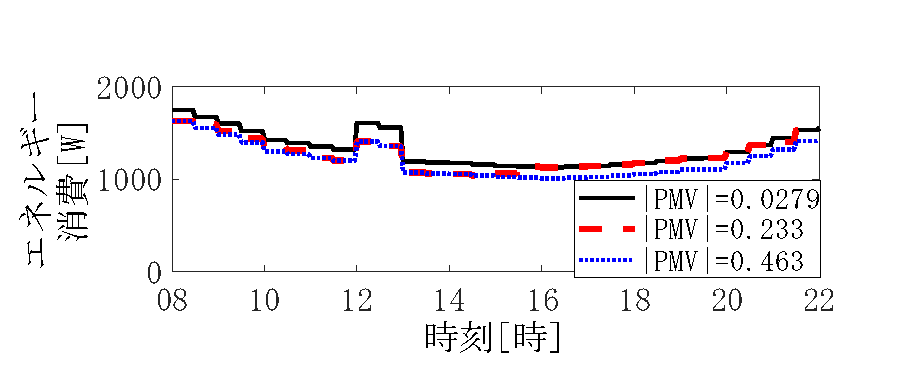
\includegraphics[width=0.6\textwidth,keepaspectratio=true]{fig/math_result_schedule_power.eps}
    \label{fig::math_result_schedule_power}
  }
  \caption{数理モデル最適化で獲得された空調設定スケジュール,室内快適性,エネルギー消費量の例}
  \label{fig::math_result_schedule}
\end{figure}
獲得された設定温度スケジュールが最も多様であった$|PMV| \approx 0.25$付近の解10個の設定温度スケジュールを確認する.それぞれの設定温度スケジュールを\figref{fig::math_result_schedule_settemp10}に示す.全体的な傾向として,どの解も15:30~17:00の時間帯は25$^o$C以上の設定温度であることがわかる.午前中は温度が低く午後に温度が高くなる解が多いが,(b)(h)のように午前中を午後よりも高い設定温度とする解や,(i)のように一日を通して設定温度がほぼ一定である解もある.また,多くの解は昼の時間帯は制約\Eqref{eq::math_constraint_pmv}を考慮せずともよくなるため設定温度が他の時間帯に対し1$^o$C程度低くなっているが,(i)の解については温度が低くなっていない.

\begin{figure*}[htbp]
  \begin{center}
    \begin{minipage}{0.4\textwidth}
      \begin{center}
        \includegraphics[width=1.0\textwidth,keepaspectratio=true]{fig/math_result_schedule_settemp_a.eps}\\\vspace{0.3cm}{{(a) $|PMV|=0.223$}}
      \end{center}
    \end{minipage}
    \begin{minipage}{0.4\textwidth}
      \begin{center}
        \includegraphics[width=1.0\textwidth,keepaspectratio=true]{fig/math_result_schedule_settemp_b.eps}\\\vspace{0.3cm}{{(b) $|PMV|=0.228$}}
      \end{center}
    \end{minipage}
    \begin{minipage}{0.4\textwidth}
      \begin{center}
        \includegraphics[width=1.0\textwidth,keepaspectratio=true]{fig/math_result_schedule_settemp_c.eps}\\\vspace{0.3cm}{{(c) $|PMV|=0.233$}}
      \end{center}
    \end{minipage}
    \begin{minipage}{0.4\textwidth}
      \begin{center}
        \includegraphics[width=1.0\textwidth,keepaspectratio=true]{fig/math_result_schedule_settemp_d.eps}\\\vspace{0.3cm}{{(d) $|PMV|=0.238$}}
      \end{center}
    \end{minipage}
    \begin{minipage}{0.4\textwidth}
      \begin{center}
        \includegraphics[width=1.0\textwidth,keepaspectratio=true]{fig/math_result_schedule_settemp_e.eps}\\\vspace{0.3cm}{{(e) $|PMV|=0.248$}}
      \end{center}
    \end{minipage}
    \begin{minipage}{0.4\textwidth}
      \begin{center}
        \includegraphics[width=1.0\textwidth,keepaspectratio=true]{fig/math_result_schedule_settemp_f.eps}\\\vspace{0.3cm}{{(f) $|PMV|=0.253$}}
      \end{center}
    \end{minipage}
    \begin{minipage}{0.4\textwidth}
      \begin{center}
        \includegraphics[width=1.0\textwidth,keepaspectratio=true]{fig/math_result_schedule_settemp_g.eps}\\\vspace{0.3cm}{{(g) $|PMV|=0.258$}}
      \end{center}
    \end{minipage}
    \begin{minipage}{0.4\textwidth}
      \begin{center}
        \includegraphics[width=1.0\textwidth,keepaspectratio=true]{fig/math_result_schedule_settemp_h.eps}\\\vspace{0.3cm}{{(h) $|PMV|=0.263$}}
      \end{center}
    \end{minipage}
    \begin{minipage}{0.4\textwidth}
      \begin{center}
        \includegraphics[width=1.0\textwidth,keepaspectratio=true]{fig/math_result_schedule_settemp_i.eps}\\\vspace{0.3cm}{{(i) $|PMV|=0.267$}}
      \end{center}
    \end{minipage}
    \begin{minipage}{0.4\textwidth}
      \begin{center}
        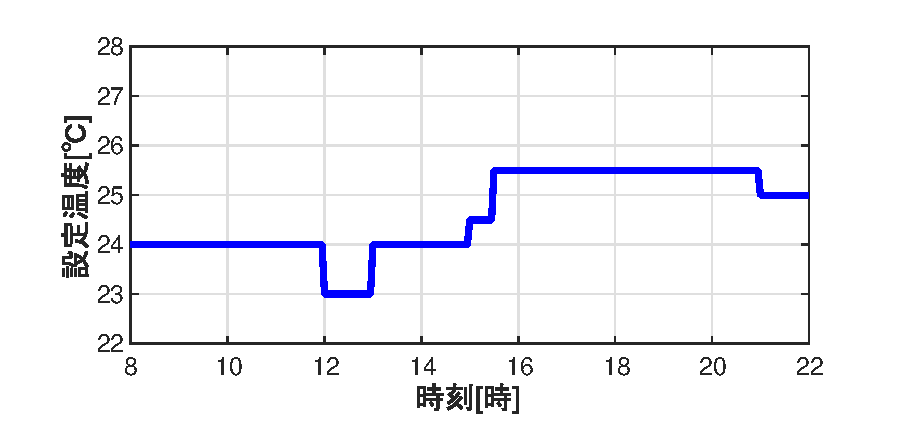
\includegraphics[width=1.0\textwidth,keepaspectratio=true]{fig/math_result_schedule_settemp_j.eps}\\\vspace{0.3cm}{{(j) $|PMV|=0.278$}}
      \end{center}
    \end{minipage}
  \end{center}
  \caption{設定温度パターンの例($\epsilon$=0)}
  \label{fig::math_result_schedule_settemp10}
\end{figure*}

本事例では,探索には\secref{sec::math_setting}で述べた計算環境において,$\epsilon=0$の場合61分3秒,$\epsilon=0.0075$の場合69分50秒, $\epsilon=0.05$の場合75分49秒で計算を終えている.この結果は,直近に配信された正確な気象情報を用いて運転に利用できる,実用的な計算時間であると言える.一方,本章ではビルの一室を対象として最適化を行ったが,ビル全体などさらに大きな規模の環境を対象とする場合は,解評価に必要な数理モデルの計算時間と最適化にかかる時間が増大することが想定される.そのため,対象をビル全体とする場合は計算の高速化が必要である.

\subsection{考察}

(a)パレート解分布\\
探索によって得られたパレート解分布は,制約範囲の境界付近($|$PMV$|\leq 0.1$と$|$PMV$|\geq 0.4$)の解の数が少なかった.これは,数理モデルに原因があると考える.本章で取り扱った数理モデルでは,一日の平均$|$PMV$|$を0もしくは0.5とするには,全ての時間帯でPMV値を0(もしくは-0.5)にしなければならず,設定温度スケジュールも一定値($|$PMV$|\approx0$とするには25.5$^o$C,$|$PMV$|\approx0.5$とするには24$^o$C)にする必要がある.そのため,制約範囲の境界に近いほど設定温度スケジュールが一定値に近くなり変更の余地が少なくなるので,制約範囲の境界付近では多様な解を探索しにくくなり,結果として獲得された解の数が少なかったものと考える.また,$\epsilon$値を大きくすると,制約範囲の境界付近の解が探索できず,解集合の分布も均等でなくなる傾向が見られた.本問題の様に境界付近で探索しにくくなる場合には,$\epsilon$値を大きくして選択圧を上げるよりも,$\epsilon$優越のような優越範囲の変更は行わず,境界付近の解も探索できるようにした方が良いと言える.

(b) 空調設定スケジュール\\
\figref{fig::math_result_schedule}より,平均$|PMV|=0.233$の場合は,各時間帯のPMV値が0に近い場合(16時~22時)と制約値である-0.5に近い場合(8時~14時)があることがわかる.
\figref{fig::math_outside_temp}を見ると,前者は外気温度が比較的高めで,後者は外気温度が低めである.本章で想定する環境条件は冬季であり,空調は暖房動作をしているため,外気温度が高ければ空調のエネルギー消費量は小さくなり,外気温度が低い場合は空調のエネルギー消費量は大きくなる.ここから,PMV値が時間帯によって違う理由は,気温が低くエネルギー消費量が大きくなる時間帯はエネルギー消費量を抑えるためPMV値を-0.5付近に制御し,気温が比較的高くエネルギー消費量が低めの時間帯は快適性を優先しPMV値を0付近に制御していたためであると考えられる.また,\figref{fig::math_result_schedule_settemp10}より,空調の設定温度スケジュールについて,平均$|PMV|=0.233$の様な午後の設定温度を午前よりも高くし昼は設定温度を下げる解以外にも,以下の解のスケジュールがあることがわかる.\\
・昼の時間帯に温度を下げず,午前午後ともに設定温度がほぼ一定であるスケジュール (i)\\
・午前を午後よりも高い設定温度とするスケジュール (b, h)\\
特に制約が無い昼の時間帯に温度を下げないスケジュールがある点や,一日のうち設定温度のピークが異なる時間帯にある解がそれぞれ得られている点から,解のスケジュールには十分な多様性や網羅性がある.そのため,提案手法によって獲得された解集合を候補とすることで,設備管理者は十分豊富な選択肢の中から計画値を決定できると言える.
また,どの解も15:30~17:00の時間は設定温度が25[$^o$C]以上となっている.これは,14時~17時の時間帯は気温が高くエネルギー消費量が低く室内快適性を優先しやすい点と,昼には設定温度を下げるため隣接時間帯との温度差の制約\Eqref{eq::math_constraint_tset_diff}により直後の13時~15時は急激に設定温度を上げられない点によるものと考える.

(c)熱負荷計算方法\\
本章で獲得された空調設定スケジュールでは,予熱運転等をしてもその効果が反映されていない.これは,本章で用いた数理モデルにおける熱負荷計算式が,設定温度・外気温度・室内の発熱のみに依存することを前提としたものであったためと考える.そのため,例えば暖房で温められた部屋の蓄熱量は考慮されずに熱負荷を計算しており,予熱等の効果は反映されなかった.そこで,予熱運転等を考慮した空調設定スケジュールを生成できるよう,熱負荷計算式を改善することや,より正確な熱の推移を計算可能なシミュレータの利用が必要である.

(d)快適性評価モデル\\
本章では,部屋の平均的な温冷感を示す快適性指標PMVを,設定温度と室内機風量設定値を用いた簡易な計算式のみによって計算していた.しかしながら,実際の室温,湿度,風速,平均放射温度は天候や在室者数によっても左右されるため,計算値と不整合が生じる.加えて,在室者の快適性は在室者の座席配置や在室者自身の体調・状況に依存して個人ごとに異なるものであり,PMVは各在室者の快適性を直接表現することができない.そのため,より実際に即した温熱快適性指標と,指標の高速で正確な推定・計算手法を合わせて,目的関数とする必要がある.

\section{ビル管理者の意思決定プロセス}\label{sec::decision_making}
中規模~大規模のオフィスビルの場合,ビル管理者がビルの空調設備を運用している.提案システムでは,室内快適性とエネルギー消費量のトレードオフを示す複数の空調設定温度スケジュールを獲得し,ビル管理者に提示する.ビル管理者は,その中から1つのスケジュールを選択して空調設備運用を行う必要がある.本節では,提案システムで得られた空調設定温度スケジュールの中から,実際に使用するスケジュールを1つ選択する場合の意思決定シナリオを紹介する.
意思決定シナリオの概要を\figref{fig::math_decision_making}に示す.

\begin{figure}[htbp]
  \begin{center}
    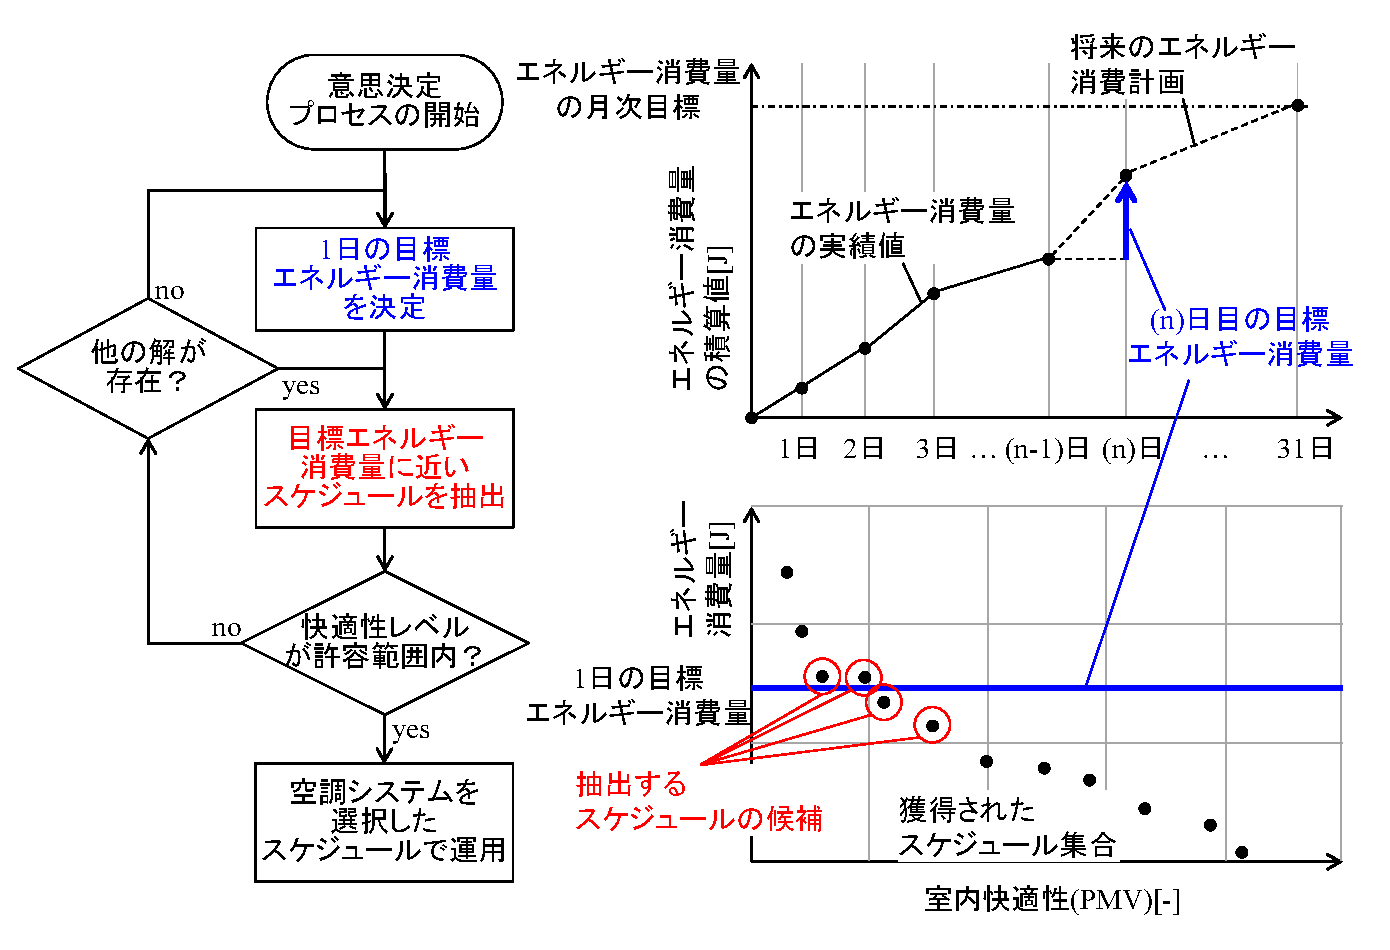
\includegraphics[width=0.8\linewidth]{fig/math_decision_making.eps}
  \end{center}
  \caption{n日目の空調設定スケジュールの意思決定シナリオ}
  \label{fig::math_decision_making}
\end{figure}

まず,ビル管理者は,昨日までの実際のエネルギー消費量と月別のエネルギー消費量の目標値とから,当日のエネルギー消費量の目標値を決定する.その処理を\figref{fig::math_decision_making}の右上に示す.青の実線がその日のエネルギー消費量の目標値を示している.次に,ビル管理者は,目的空間内の最適化されたスケジュールのプロットから,その日の目標エネルギー消費量以下またはそれに近いスケジュールを1つ抽出する.\figref{fig::math_decision_making}の右下に示した赤丸で囲んだスケジュールが,抽出される可能性のあるスケジュールである.すでに目標エネルギー消費量を決定しているので,基本的には目標エネルギー消費量に近いスケジュールを選ぶべきであり,省エネでも快適性が悪いスケジュールを選択する必要はない.その後,ビル管理者は,部屋間の快適性のばらつきをチェックする.許容できるレベルでない場合には,目標エネルギー消費量を中心とした別のスケジュールを選択し,快適性を確認する.目標エネルギー消費量以下のスケジュールがない場合は,その日のエネルギー消費量の目標値を増やして,再度抽出する必要がある.最後に,ビル管理者は,選択された空調設定温度スケジュールで空調システムを運用する.
このように,提案システムは,動的な温度設定スケジュール集合を生成するだけでなく,一日のエネルギー消費量目標値を達成するための意思決定支援も行うことができる.これにより,オフィスワーカーの快適性を維持しつつ,エネルギー消費量の削減に貢献することができる.

\section{結言}
本章では,オフィスの一室の空調設定スケジュールを,数理モデルを用いて最適化する手段について述べた.室内快適性の向上と1日のエネルギー消費量の削減の2つを目的とし,目的関数を数理モデルを用いて定式化した.数理モデルに対してOMOPSOアルゴリズムを適用して,空調設定スケジュールの非劣解集合を探索した.選択圧を変更するパラメータ$\epsilon$を$\epsilon=0$とすることで,エネルギー消費量を削減し快適性を向上できるスケジュールを複数獲得できた.獲得したスケジュール集合は目的関数で広い範囲の解を含んでおり,ビル管理者による意思決定支援が可能であることを示した.

一方で,ビル全体を数理モデル化することに困難がある.本章では,オフィスの一室を数理モデル化したが,数理モデル化の手続きをビル全体に適用する場合,異なる特性を持つ室・熱負荷・設備機器をビルの各部屋に対して設定しなければならない.また,本章では,温湿度,風速等の環境計測値やパラメータの一部に仮定値を用いたが,本来,これらの値は室ごとに空調機と室内の熱移動を考慮して算出する必要がある.そのため,本章の数理モデルをそのままビル全体へ拡張しようとすると,ビルの規模が大きくなるにつれて,正確な数理モデル化が困難になる.

ビル全体の空調最適化のためには,部屋などの相互関係を考慮して室内快適性とエネルギー消費量を正確に評価する手段が必要になる.次章では,ビル全体の室内快適性およびエネルギー消費量を計算・評価する手段としてビルシミュレータを採用し,本章で述べた数理モデルをビルシミュレータによって代替する試みについて述べる.



\chapter{シミュレーション最適化 }
\label{chap::sim}

\hspace{1zw}この章ではビル全体の空調設定スケジュールを最適化するために,ビルシミュレータを用いる手段について述べる.

\section{概要}
最適化システムの構成を\figref{fig::sim_system}に示す.\figref{fig::math_system}の評価部における数理モデルの代替として,ビルシミュレータEnergyPlus \cite{NREL19}を用いる.EnergyPlusは,米国エネルギー省再生可能エネルギー研究所(NREL)が開発した建築物のエネルギーシミュレータであり,建物内外の熱移動とそれに伴う温湿度変化,空調,換気,照明等各設備のエネルギー消費量を算出できる.EnergyPlusは,ビル躯体の構造・設備・エネルギー使用設定等の建物情報,外気温・外気湿度・天候・日射量などの気象情報,空調設定温度スケジュール情報を入力することで,エネルギー消費量や各部屋の環境および快適性の時系列データを算出できる.\chapref{chap::math}における数理モデルをEnergyPlusによるシミュレーションで代替することで,部屋単位の詳細な数理モデルの構築を回避する.EnergyPlusシミュレータでシミュレーションを行うためには,シミュレータにシミュレーション対象のビルモデルを入力する必要がある.本論文では,建築用のモデリングソフトウエアRevitを用いて,ビルの構造,設備,エネルギー設定等を含むオフィスビルのモデルを構築する.

\begin{figure*}[t]
  \begin{center}
    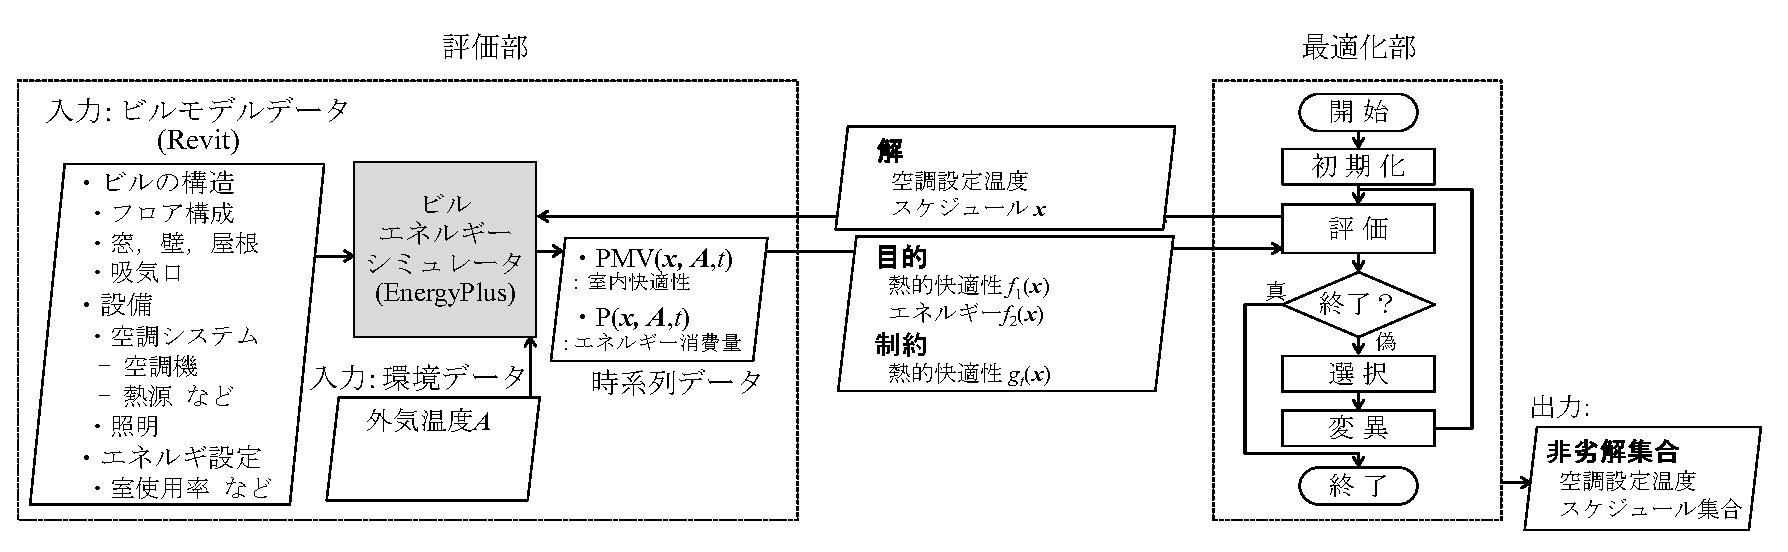
\includegraphics[width=1.1\linewidth]{fig/sim_system.eps}
  \end{center}
  \caption{シミュレーション最適化システム}
  \label{fig::sim_system}
\end{figure*}


\section{シミュレーション最適化における解評価}\label{sec::sim_model}
\subsection{ビルのモデルとシミュレーション}
本章の最適化対象は,オフィスの一室ではなく,ビル全体である.本研究で作成したシミュレーション対象のオフィスビルのモデルを\figref{fig::sim_office_building}に示す.また,主な諸元を\tabref{tab::sim_description}に,1階のフロアレイアウト\figref{fig::sim_groundfloor}に,基準階のフロアレイアウトを\figref{fig::sim_typicalfloor}に示す.このビルは,地上8階建てで,延床面積が11,781$[m^2]$であり,全フロアにオフィスを持つ.ビル内のオフィス数は54,室内快適性とエネルギー消費量の解析対象にする空間数は,廊下,トイレ,エレベータホールなども含めて114とした.また,エネルギー解析のための設定を\tabref{tab::sim_analysis_param}に示す.本ビルにはセントラル空調システムが導入されており,冷温水を用いて各フロアの空調機が冷風と温風を作り,可変風量ユニットを経由して各部屋に供給する.

\begin{figure}[htbp]
  \begin{center}
    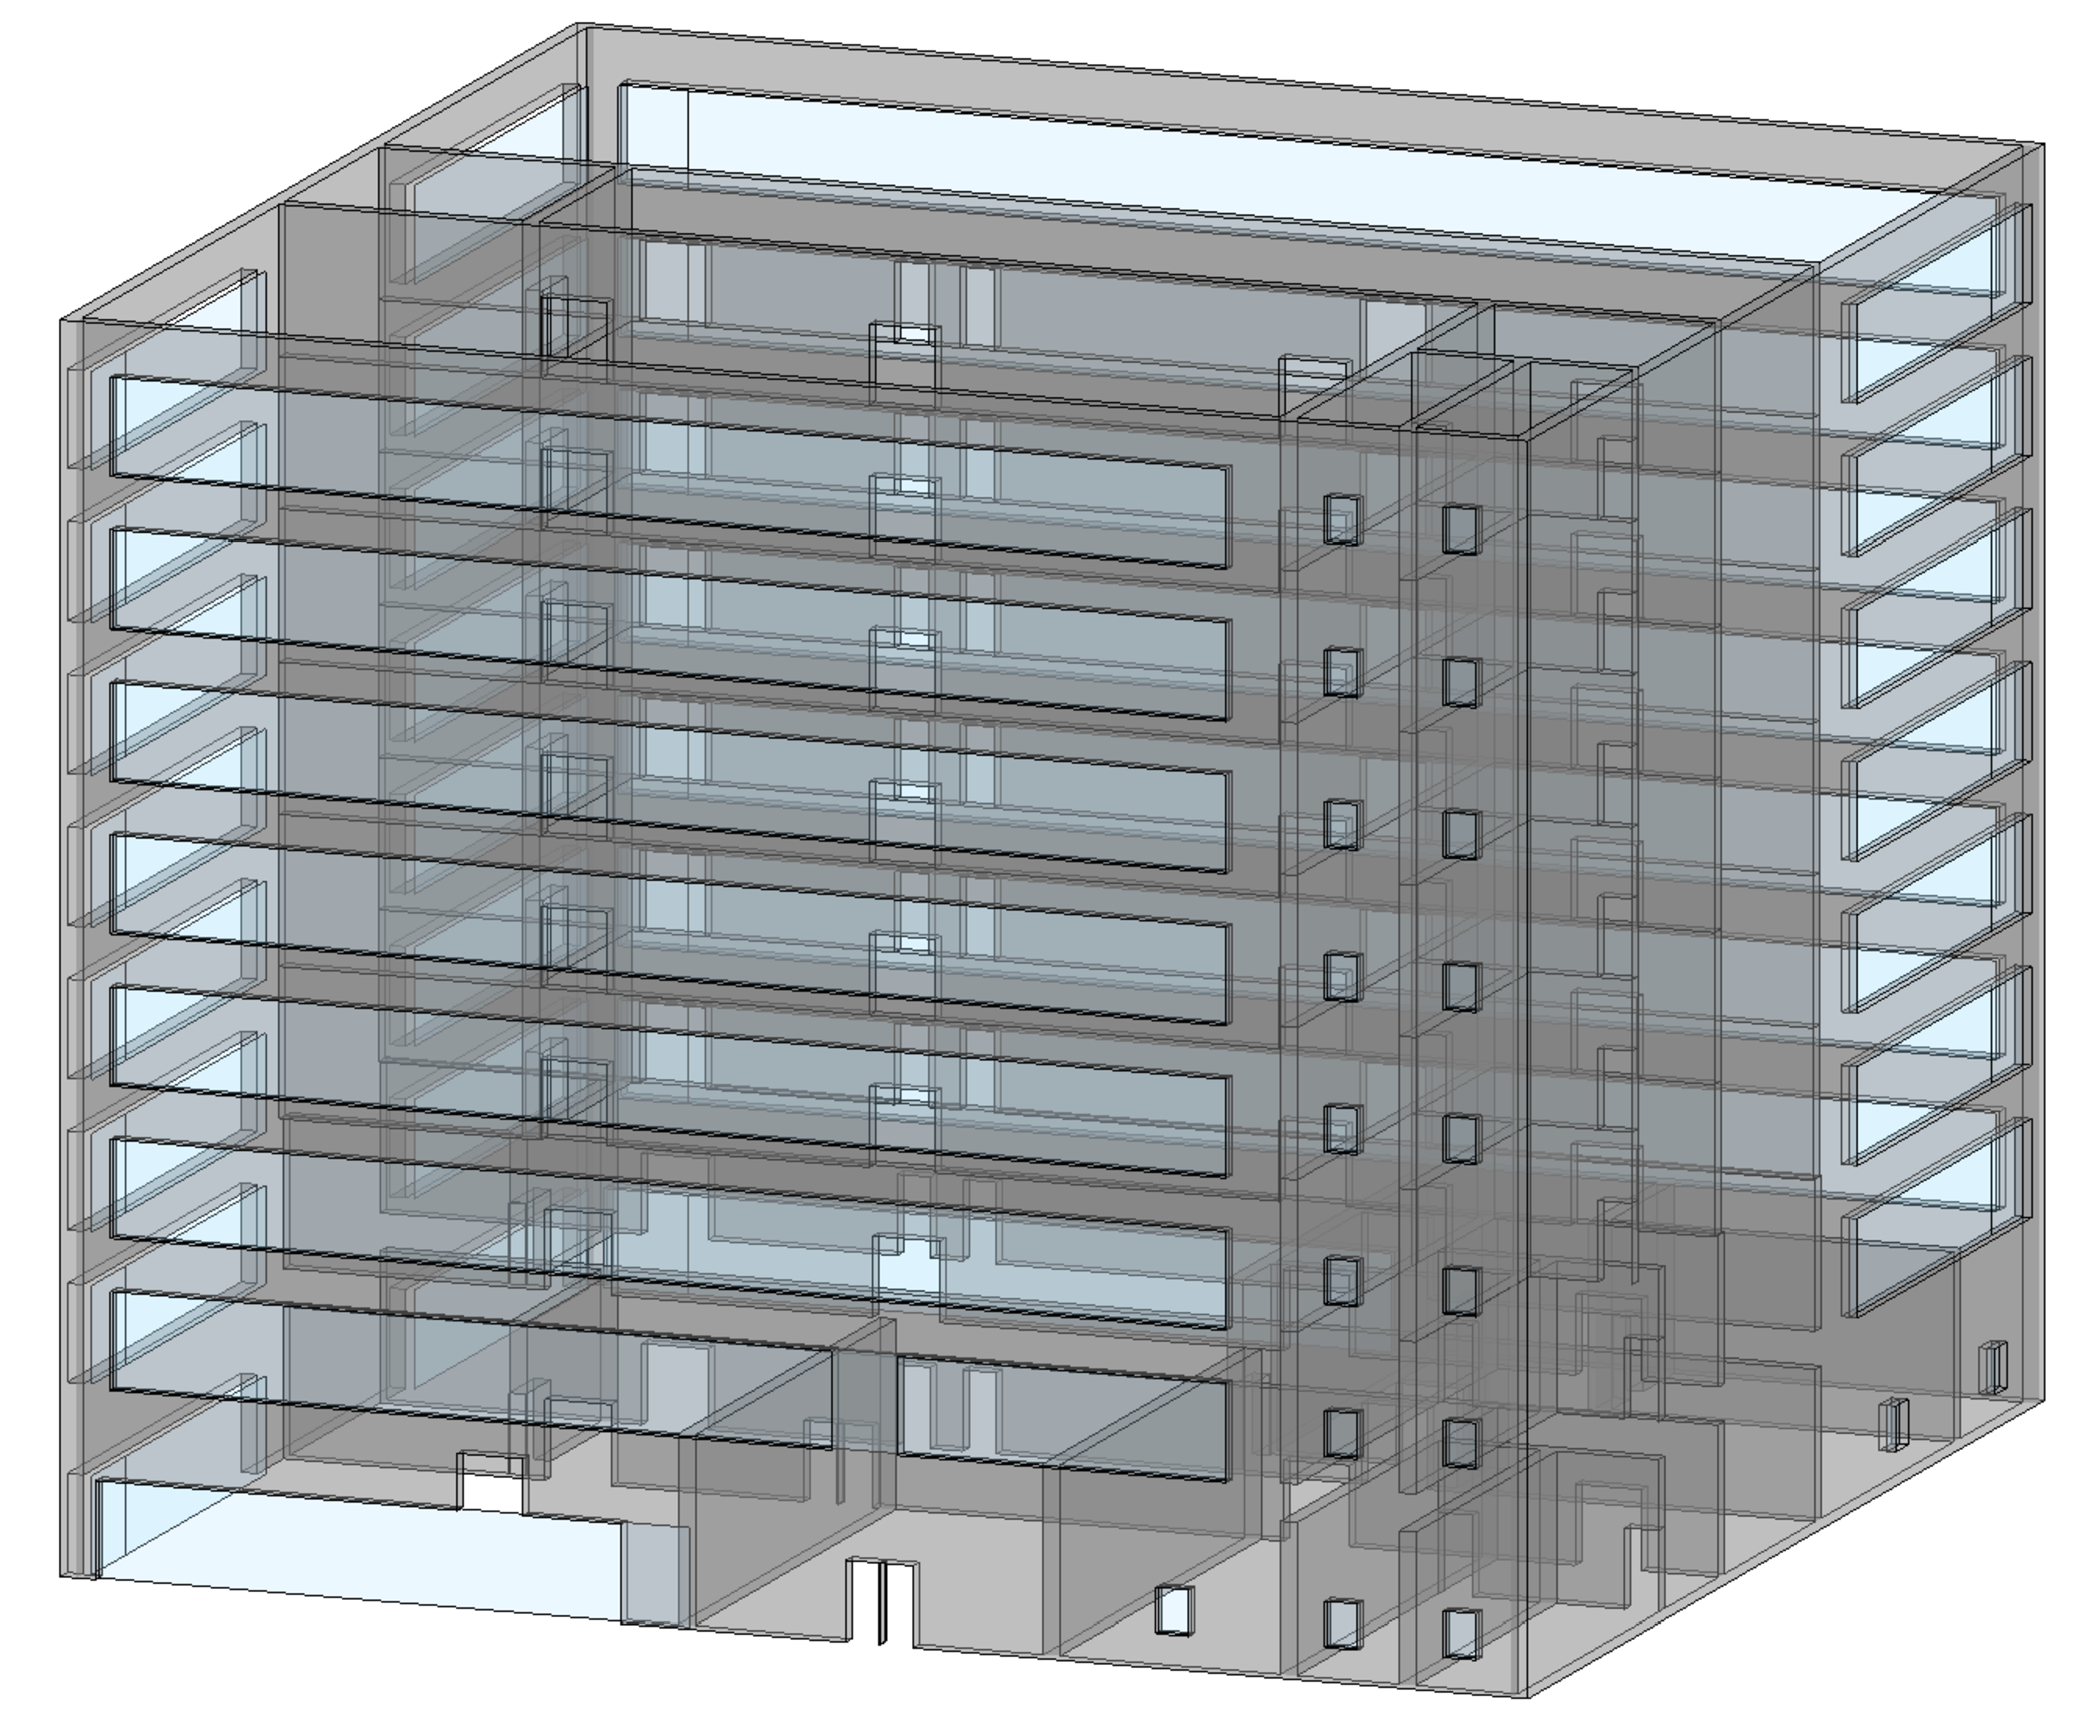
\includegraphics[width=0.6\linewidth]{fig/sim_office_building.eps}
  \end{center}
  \caption{最適化対象のオフィスビルモデルの外観}
  \label{fig::sim_office_building}
\end{figure}

\begin{table}[htbp]
  {\small
    \begin{center}
      \caption{最適化対象のオフィスビルの主要諸元}
      \label{tab::sim_description}
      \begin{tabular}{c|cccc}
        \hline
        項目     & 値                 \\
        \hline \hline
        建物用途 & オフィスビル       \\
        構造     & 鉄筋コンクリート造 \\
        敷地面積 & 5,000 [m$^2$]      \\
        建築面積 & 1,508 [m$^2$]      \\
        延床面積 & 11,781 [m$^2$]     \\
        階数     & 8                  \\
        \hline
      \end{tabular}
    \end{center}
  }
\end{table}

\begin{figure}[htbp]
  \begin{center}
    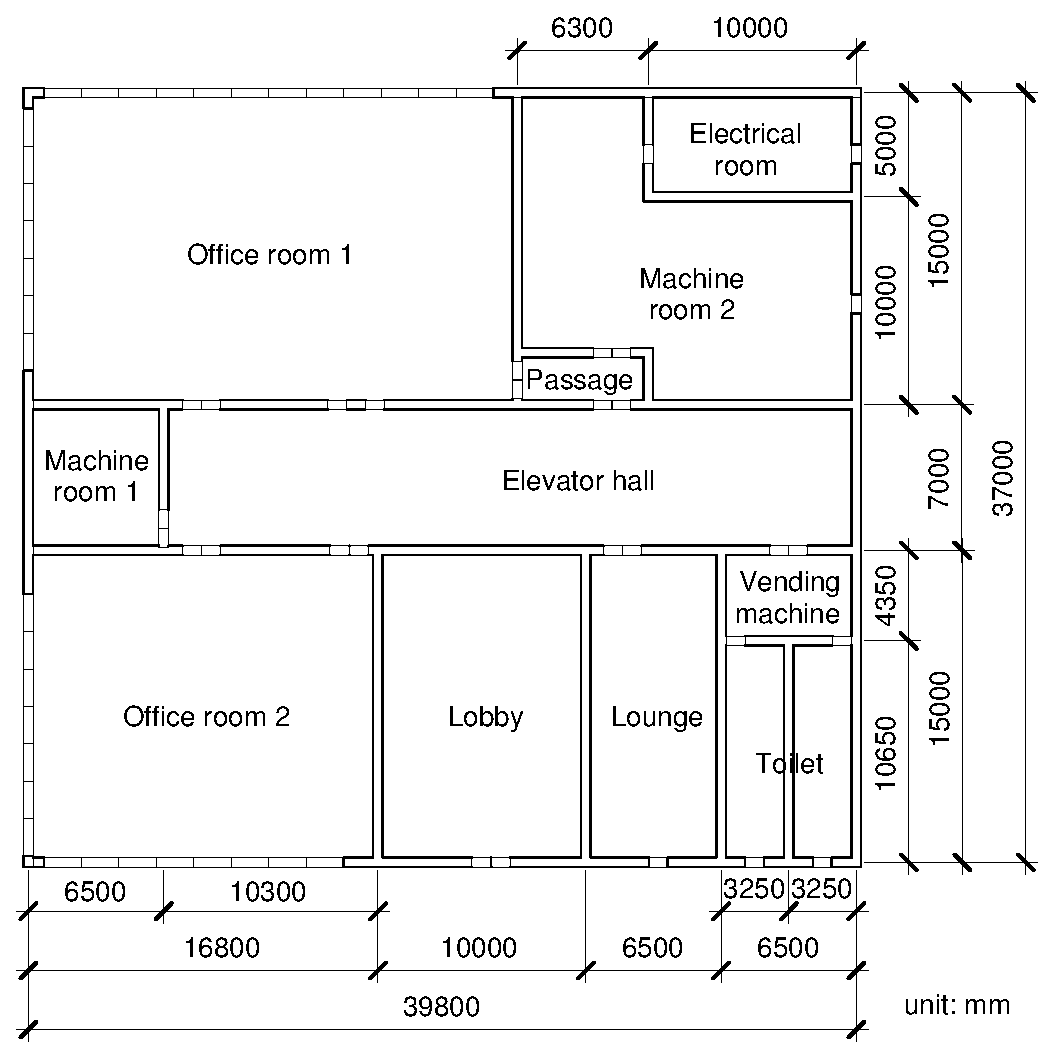
\includegraphics[width=0.65\linewidth]{fig/sim_groundfloor_en.eps}
  \end{center}
  \caption{1階のフロアレイアウト}
  \label{fig::sim_groundfloor}
\end{figure}
\begin{figure}[ht]
  \begin{center}
    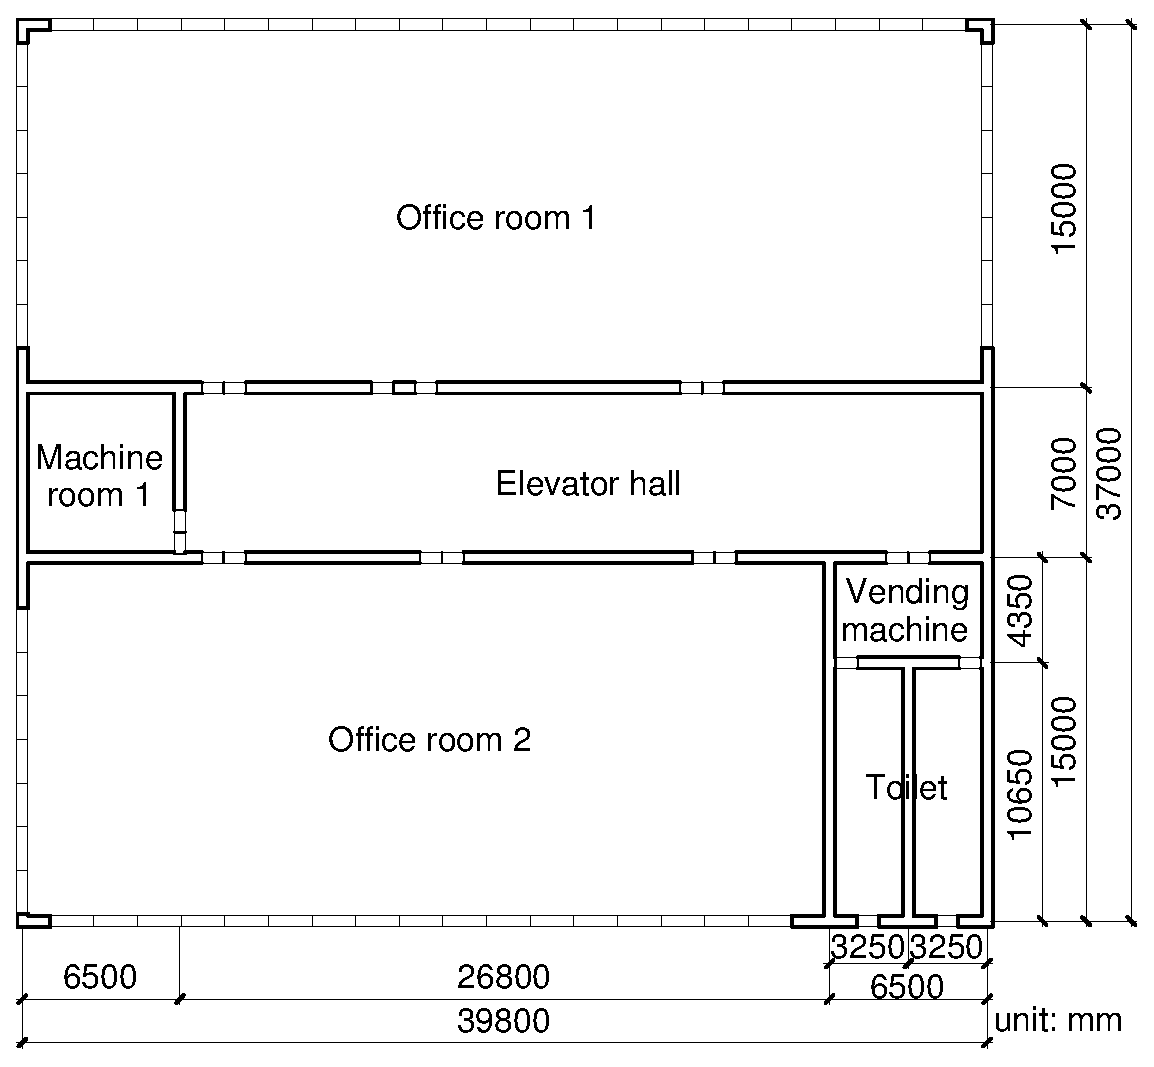
\includegraphics[width=0.65\linewidth]{fig/sim_typicalfloor_en.eps}
  \end{center}
  \caption{基準階のフロアレイアウト}
  \label{fig::sim_typicalfloor}
\end{figure}


\begin{table}[htbp]
  {\small
    \begin{center}
      \caption{エネルギー解析設定}
      \label{tab::sim_analysis_param}
      \begin{tabular}{c|cccc}
        \hline
        設定項目                     & 値                                      \\
        \hline \hline
        \raisebox{2mm}{外壁断熱材}   & \shortstack{発泡ポリスチレンフォーム    \\ (R値 \footnotemark[1] = 1.73 [m$^2$ K/W]) }\\
        \raisebox{2mm}{屋根断熱材}   & \shortstack{発泡ポリスチレンフォーム    \\ (R値 = 3.87 [m$^2$ K/W]) }\\
        \raisebox{2mm}{窓}           & \shortstack{Low-Eペアガラス             \\ (低日射熱取得率タイプ)}\\
        \raisebox{5mm}{空調システム} & \shortstack{中央熱源方式                \\冷温水機(COP \footnotemark[2]=5.96) \\ 可変風量システム}\\
        外気導入量                   & 1.38 [$ LPS$ \footnotemark[3]$ / m^2 $] \\
        人体発熱量                   & 顕熱: 55 ,  潜熱: 64 [W/人]             \\
        \shortstack{執務者の                                                   \\占有面積} & \raisebox{2mm}{10 [m$^2$/人]} \\
        照明発熱量                   & 10.6 [W/m$^2$]                          \\
        電気機器発熱量               & 12 [W/m$^2$]                            \\
        \hline
      \end{tabular}
    \end{center}
  }
\end{table}

\subsection{設計変数}
本章では,\chapref{chap::math}と同様に,空調設定温度スケジュール$t_{set}(\vec{x},t)$を最適化する. 本章では,分割時間間隔$T_s=1$[hour]として,設定可能時刻集合を$\mathcal{T}_{set}=\{5:00, 6:00,\dots, 24:00\}$とする.また設定温度スケジュールを設計変数ベクトルで表す方法として,\Eqref{eq::math_variable_diff}と同じ形式の\Eqref{eq::sim_variable_diff}を用いる.
\begin{align}
  t_{set}(\vec{x},t) & =
  \begin{cases}
    x_t ~~~~~~~~~~~~~~                          & (t=5:00)                 \\
    t_{set}(\vec{x},t-T_s) + x_t ~~~~~~~~~~~~~~ & (t=6:00, 7:00,...,24:00) \\
  \end{cases}
  \label{eq::sim_variable_diff}
\end{align}

\subsection{目的関数}
ビルシミュレータであるEnergyPlusは,各時刻$t$における室内快適性を$TCFM(\vec{x},\mathcal{A},t)$ (TCFM: Thermal Comfort Fanger Model),空調システムの電力エネルギー消費量を$ASEE(\vec{x},\mathcal{A},t)$   (ASEE: Air System Electric Energy)として出力する.これらの値を用いて,第一目的関数である\Eqref{eq::math_objective1}, 第二目的関数である\Eqref{eq::math_objective2},制約関数である\Eqref{eq::math_constraint_pmv}における,室内快適性$PMV(\vec{x},\mathcal{A},t)$, エネルギー消費量$P(\vec{x},\mathcal{A},t)$を以下のように代替して算出する.
\begin{align}
  PMV(\vec{x},\mathcal{A},t) & = TCFM(\vec{x},\mathcal{A},t)
  \label{eq::sim_pmv}
\end{align}
\begin{align}
  P(\vec{x},\mathcal{A},t) & = ASEE(\vec{x},\mathcal{A},t)
  \label{eq::sim_asee}
\end{align}

EnergyPlusは室内快適性,エネルギー消費量を10分毎のデータとして出力する.そこで,快適性評価対象の時刻は$\mathcal{T}_1=\{7:00, 7:10,\dots, 20:50, 21:00\}$,エネルギー消費量評価対象時刻$\mathcal{T}_2=\{0:00, 0:10,\dots, 24:00\}$とする.また,外気温データも同様に$\mathcal{A}=\{a_{00:00},a_{00:10},\dotsc,a_{23:50},a_{24:00}\}$を使用する.

%footnote in the table
\footnotetext[1]{断熱材の熱抵抗を示す値}
\footnotetext[2]{熱源機のエネルギー効率を表す係数}
\footnotetext[3]{リットル毎秒}

\subsection{制約条件}
快適性に関する制約は,\chapref{chap::math}に記載の\eqref{eq::math_constraint_pmv}と同様とする.また,シミュレーション対象ビルの空調設備は,設定温度範囲の上下限値は\Eqref{eq::math_constraint_tset_minmax}と同様とするが,設定可能な温度幅は0.1[$^o$C]刻みとし,隣接時間帯の設定温度変更は$\pm $2[$^o$C]以内とする.そこで,空調設定温度に関する制約\Eqref{eq::math_constraint_tset_int}と\Eqref{eq::math_constraint_tset_diff}を以下の2つの式で置き換える.以降の\chapref{chap::robust},\chapref{chap::surrogate}も同様とする.
\begin{eqnarray}
  10 t_{set}(\vec{x},t) \in & \bf{Z}
  \label{eq::sim_constraint_tset_int} \\
  |t_{set}(\vec{x},t) - t_{set}(\vec{x},t-T_s)| \leq & 2
  \label{eq::sim_constraint_tset_diff}
\end{eqnarray}

\section{実験内容}\label{sec::sim_setting}
本章では,提案する空調最適化システムと従来の空調システムの一日における性能を比較する.従来の空調システムは,一定の設定温度を用いるものとする\cite{Inouye08, Kuki16}.これに対し,提案する空調最適化システムは,時間によって動的に設定温度を変化させる.この設定温度変更のスケジュールを,\subsecref{subsec::OMOPSO}で述べたOMOPSOによって探索する.従来の空調システムの結果は,提案システムと同様にシミュレータに一定の設定温度を入力することによって取得する.本節では評価シミュレーション部と最適化部の実験設定について述べる.

\subsubsection{評価シミュレーション部の設定}
本章ではシミュレーションの対象日として,一年間でエネルギー消費量が最も高まる夏期の代表日に注目する.気象データとして,2006年8月21日の東京における気象データシステム株式会社の提供する拡張アメダス(AMeDAS: Automated Meteorological Data Acquisition System)データ\cite{Akasaka00}を用いる.当日の外気温の時間推移を\figref{fig::sim_outside_temp}に示す.空調システムは冷房モードにし,設定温度の下限$x^{min}$を18[$^o$C],上限$x^{max}$を30[$^o$C]にする.また,シミュレーションでは実際のオフィスビルの利用を想定し,人体熱負荷や照明発熱,換気量について,在室者数変化を考慮して変更する.本研究では,オフィスビルのテナントの出退勤時刻を8時~17時と想定し,照明と部屋の使用率の時間推移を\figref{fig::sim_occupancy}の通りとする.

\begin{figure}[ht]
  \begin{center}
    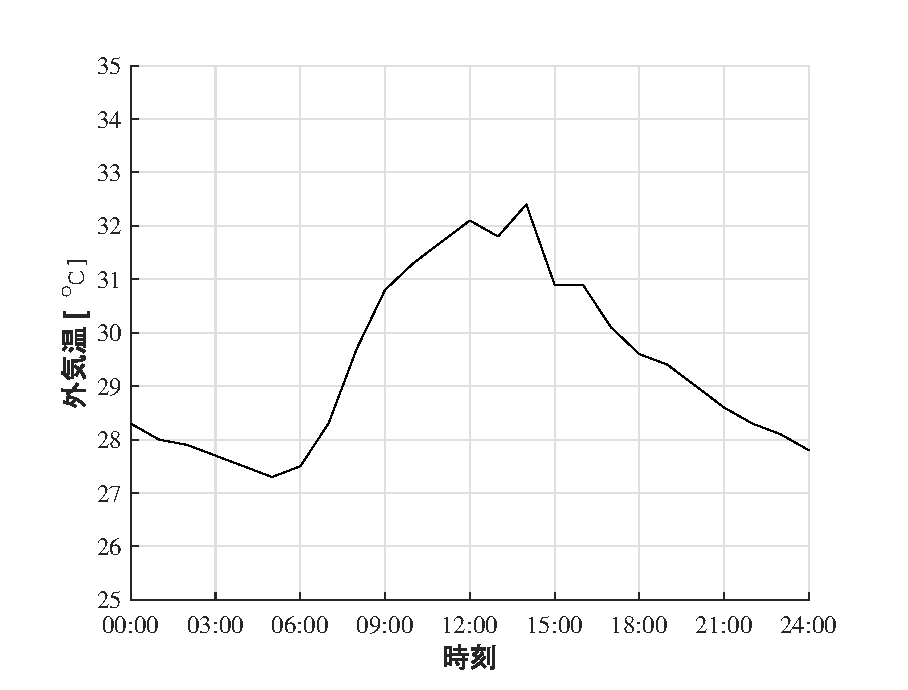
\includegraphics[width=0.7\linewidth]{fig/sim_outside_temp.eps}
  \end{center}
  \caption{一日の外気温の時間推移}
  \label{fig::sim_outside_temp}
\end{figure}

\begin{figure}[t]
  \begin{center}
    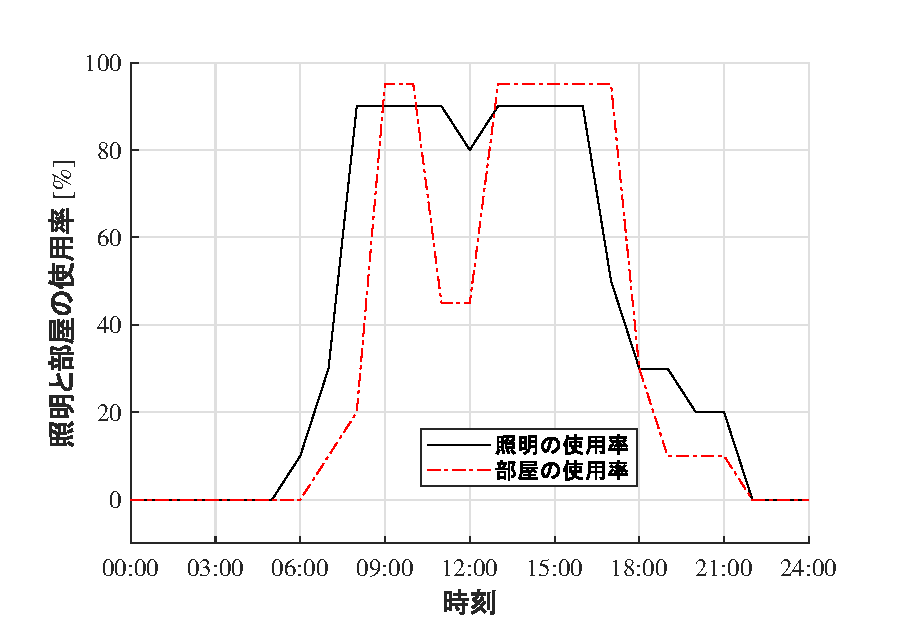
\includegraphics[width=0.7\linewidth]{fig/sim_occupancy.eps}
  \end{center}
  \caption{一日の照明と部屋の使用率の時間推移}
  \label{fig::sim_occupancy}
\end{figure}

\subsubsection{最適化部の設定}
OMOPSOで用いるパラメータを\tabref{tab::sim_param_omopso}に示す.本章では,EnergyPlusのシミュレーションを実行するプログラムとOMOPSOアルゴリズムをプログラミング言語Javaで実装した.計算機環境には,Windows 7 (64ビット),Intel Core i7-4790 (3.6GHz)およびRAM 8GBを用いた.

\begin{table}[ht]
  {\small
    \begin{center}
      \caption{OMOPSOのパラメータ}
      \label{tab::sim_param_omopso}
      \begin{tabular}{c|cccc}
        \hline
        パラメータ                             & 方法 / 値              \\
        \hline \hline
        ベース粒子群サイズ $N^{\mathcal{P}}$   & 50                     \\
        リーダー粒子群サイズ $N^{\mathcal{L}}$ & 100                    \\
        アーカイブ粒子群サイズ                 & 制限なし               \\
        総世代数 $g_{max}$                     & 500                    \\
        変数長 $n$                             & 20                     \\
        突然変異率 $p_m$                       & $1/n$                  \\
        重み $w$                               & [$0.1, 0.5$)の一様乱数 \\
        重み $c_1, c_2$                        & [$1.5, 2.0$)の一様乱数 \\
        非一様突然変異の係数 $b$               & 5 \cite{Esquivel03}    \\
        $\epsilon$-dominanceの係数$\epsilon$   & 0.0075                 \\
        \hline
      \end{tabular}
    \end{center}
  }
\end{table}


\section{実験結果}
\subsection{得られた空調設定スケジュール集合の目的関数値}
提案する空調最適化システムによって得られた設定温度スケジュール群の目的関数空間における分布を\figref{fig::sim_result_pareto}に示す.一つひとつの点が,一日の設定温度スケジュールであり,横軸を第1目的関数値の室内快適性,縦軸を第2目的関数値のエネルギー消費量とする空間にプロットされている.両方の目的関数値は,小さいほど良い結果と判断する.黒い点群は,提案する空調最適化システムによって一括獲得された最終世代のアーカイブ非劣粒子(設定温度スケジュール)群$\mathcal{E}$であり,粒子数は120だった.赤い×の点群は,従来システムとして,提案システムと同様に,エネルギーシミュレータに対して時間によらず設定温度が一定であるスケジュールを入力した場合の,快適度およびエネルギー消費量の算出結果である.

\figref{fig::sim_result_pareto}の結果から,提案法が,室内快適性およびエネルギー消費量のトレードオフを考慮した設定温度スケジュール集合を獲得できることがわかる.次に,動的に設定温度を変更する提案システムと設定温度を一定にする従来システムのスケジュールを比較する.一定の設定温度25.5[$^o$C]を用いる従来システムを除いて,提案システムは,室内快適性とエネルギー消費量の両方において,従来システムをパレート支配するスケジュールを獲得できることがわかる.

提案システムで得られたスケジュールBと温度設定を一定にする従来システムによるスケジュールDを比較する.提案システムによるスケジュールBは,従来システムによるスケジュールDと室内快適性は同程度だが,エネルギー消費量を約1.6\%削減できている.さらに,提案システムは,従来システムでは達成できない良好な室内快適性とエネルギー消費量のスケジュールを多数獲得できることがわかる.これは,双方の目的を両立するためには,設定温度を動的に変化させることが効果的であること,提案システムが適切な設定温度スケジュールを獲得できることを示している.
一方,一定温度25.5[$^o$C]を用いる従来システムによるスケジュールEは,提案システムによって得られたスケジュール集合ではパレート支配できない.しかし,一定温度25.5[$^o$C]を用いるスケジュールEは,室内快適性に関する制約条件\Eqref{eq::math_constraint_pmv}を満たさないことが確認された.すなわち,提案システムにおいて,スケジュールEは実行不可能解になる.そのため,提案システムは,従来システムによるスケジュールEをパレート支配するスケジュールを獲得できなかったと考えられる.

提案システムが獲得したスケジュールの効果をエネルギー消費量と快適性の2つの観点から試算する.従来法のスケジュールDを,同程度の快適性を示す提案法のスケジュールで置き換えると,エネルギー消費量を1日あたり$2.63×10^8$[J]削減できる.エネルギーが全て電力で賄われており,同様のエネルギー消費量削減を1年間継続できたとすると,1年間の電力消費量を約6,560[kWh],CO2排出量を3,850[kg]削減でき,オフィスビルの管理者に課せられたエネルギー消費量およびCO$_2$排出量の削減に貢献できる.また,同時に電気料金は1年間で約115,000円削減され,ビルオーナーの求める経済性にも寄与する.このシステムを全国のオフィスビルに適用でき,面積あたりの削減効果が同様だったとすると,全国のオフィスビルの総面積は約13,000[万$m^2$]である\cite{Fudoken19}ことから,全国で年間約12.7億円相当の電気料金削減と約42,400[t]のCO2排出量削減が可能である.一方で,従来のスケジュールDを同程度のエネルギー消費量の提案法のスケジュールで置き換えると,快適度が0.07向上する.これは,快適度が不快側であった場合に比べて0.875\%のオフィスワーカーの生産性改善につながる\cite{Iwahashi14, WGBC14}.今回の対象ビルのオフィスワーカーの人数は827人であり,それぞれに平均年収と同額の人件費(441万円)\cite{NTA19}がかかっている場合,約2,130万円の生産性改善効果が見込める.このシステムを全国のオフィスビルに適用できると,全国で約1,000万人存在するオフィスワーカー\cite{Fudoken19, Xymax19}全体で約2,720億円の生産性改善効果があると考えられる.

これらの結果から,提案システムは,従来システムによる一定温度設定より,室内快適性とエネルギー消費量が良好な設定温度スケジュールを獲得できることが明らかになった.

\begin{figure}[htbp]
  \begin{center}
    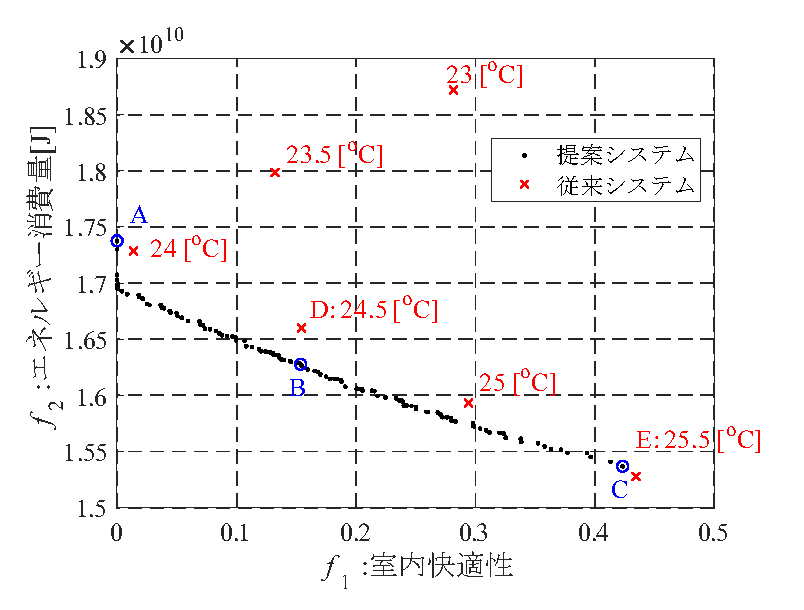
\includegraphics[width=0.7\linewidth]{fig/sim_result_pareto.eps}
  \end{center}
  \caption{シミュレーション最適化の結果}
  \label{fig::sim_result_pareto}
\end{figure}

\begin{figure*}[htbp]
  \begin{center}
    \begin{minipage}{0.5\textwidth}
      \begin{center}
        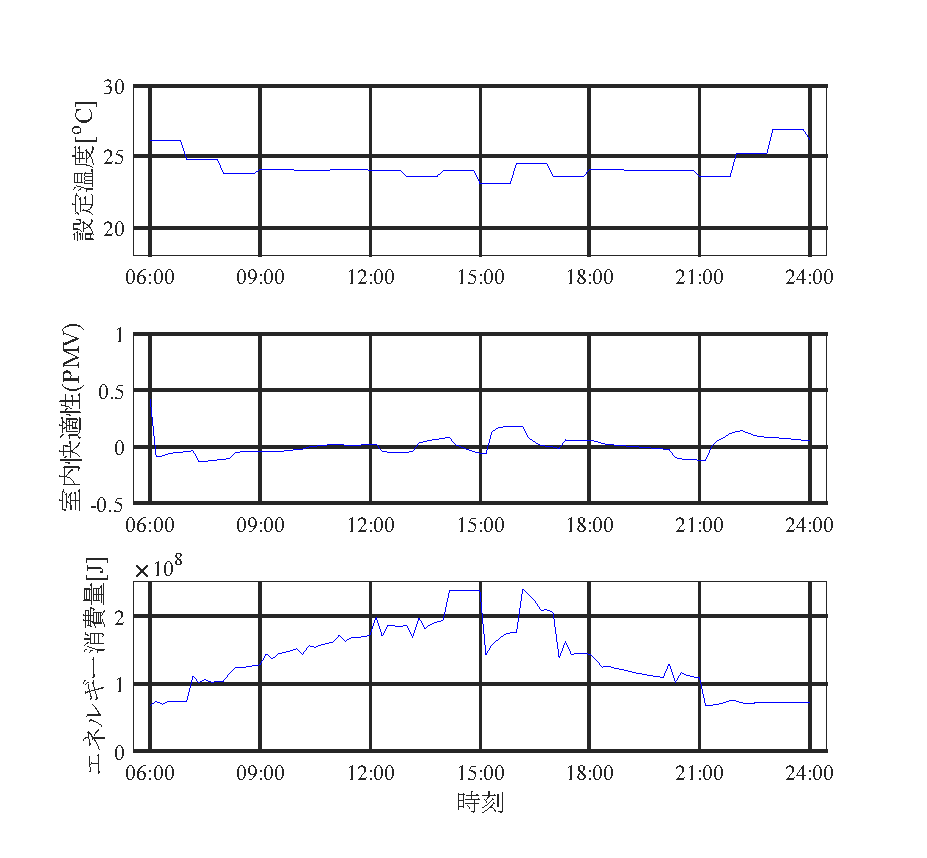
\includegraphics[width=1.0\textwidth,keepaspectratio=true]{fig/sim_result_schedule_a.eps}\\\vspace{-2mm}{スケジュール A (室内快適性が最も良い解)}
      \end{center}
    \end{minipage}
    \begin{minipage}{0.5\textwidth}
      \begin{center}
        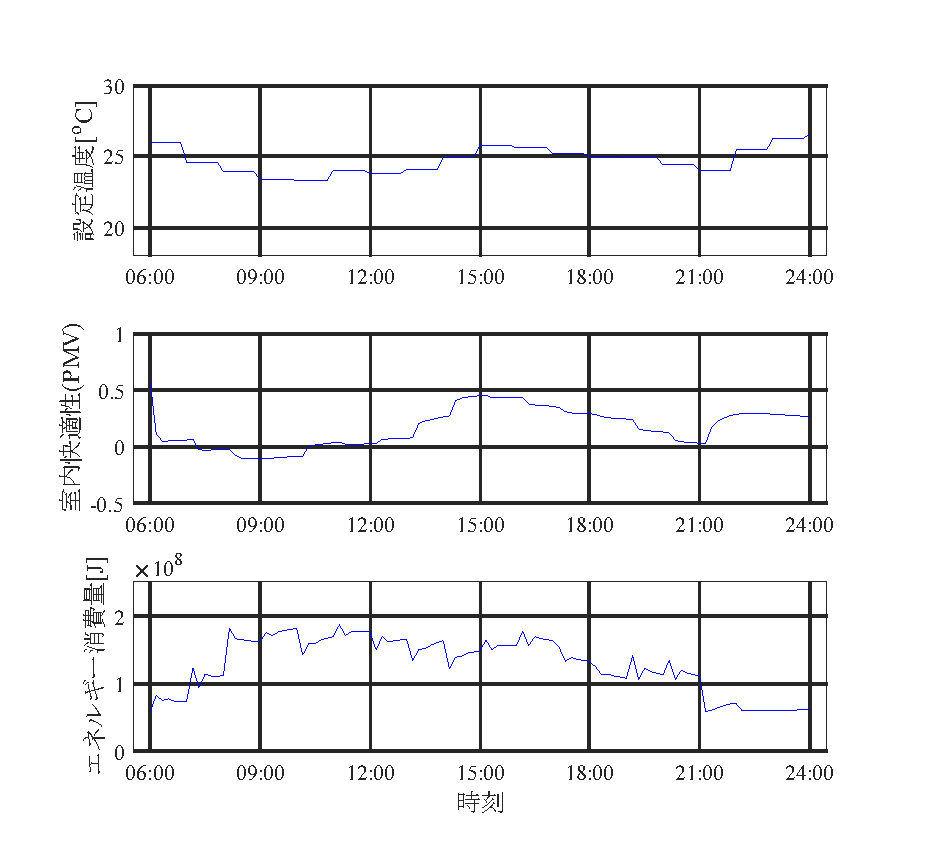
\includegraphics[width=1.0\textwidth,keepaspectratio=true]{fig/sim_result_schedule_b.eps}\\\vspace{-2mm}{スケジュール B (中間の解)}
      \end{center}
    \end{minipage}
    \begin{minipage}{0.5\textwidth}
      \begin{center}
        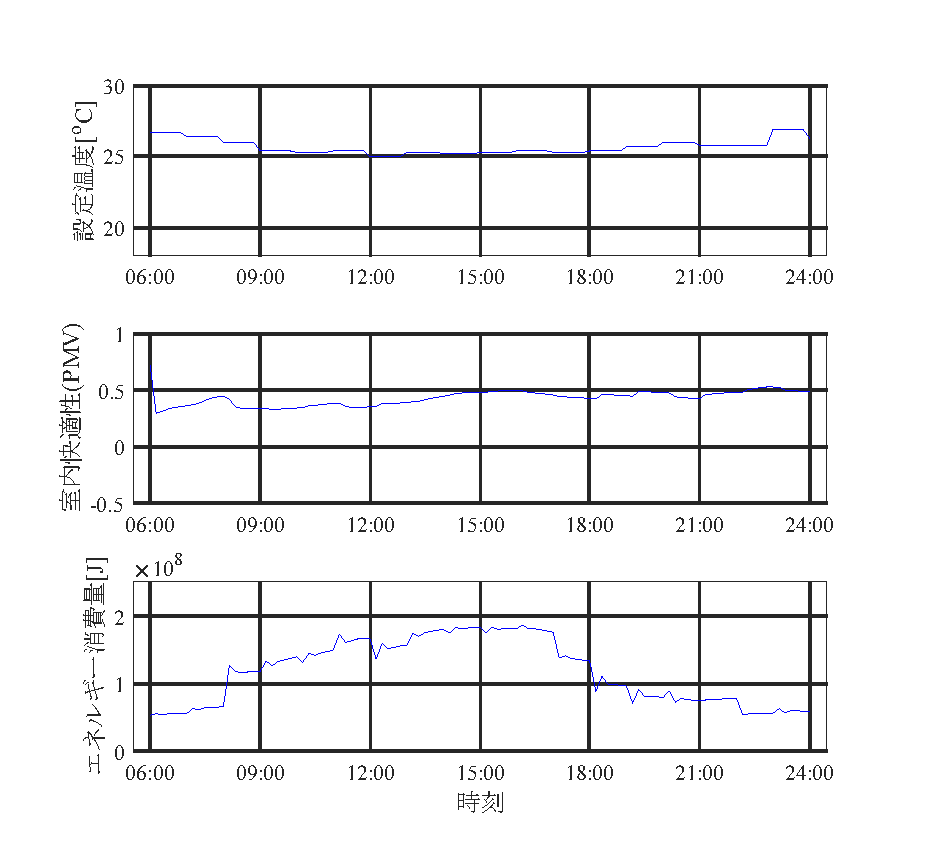
\includegraphics[width=1.0\textwidth,keepaspectratio=true]{fig/sim_result_schedule_c.eps}\\\vspace{-2mm}{スケジュール C (室内快適性が最も悪い解) }
      \end{center}
    \end{minipage}
  \end{center}
  \vspace{-2mm}
  \caption{提案システムで得られた設定温度スケジュールによる結果}
  \label{fig::sim_result_schedule}
\end{figure*}

\begin{figure*}[htbp]
  \begin{center}
    \begin{minipage}{0.5\textwidth}
      \begin{center}
        \includegraphics[width=1.0\textwidth,keepaspectratio=true]{fig/sim_result_schedule_d.eps}\\{スケジュール D (設定温度24.5[$^o$C])}
      \end{center}
    \end{minipage}
    \hspace{2cm}
    \begin{minipage}{0.5\textwidth}
      \begin{center}
        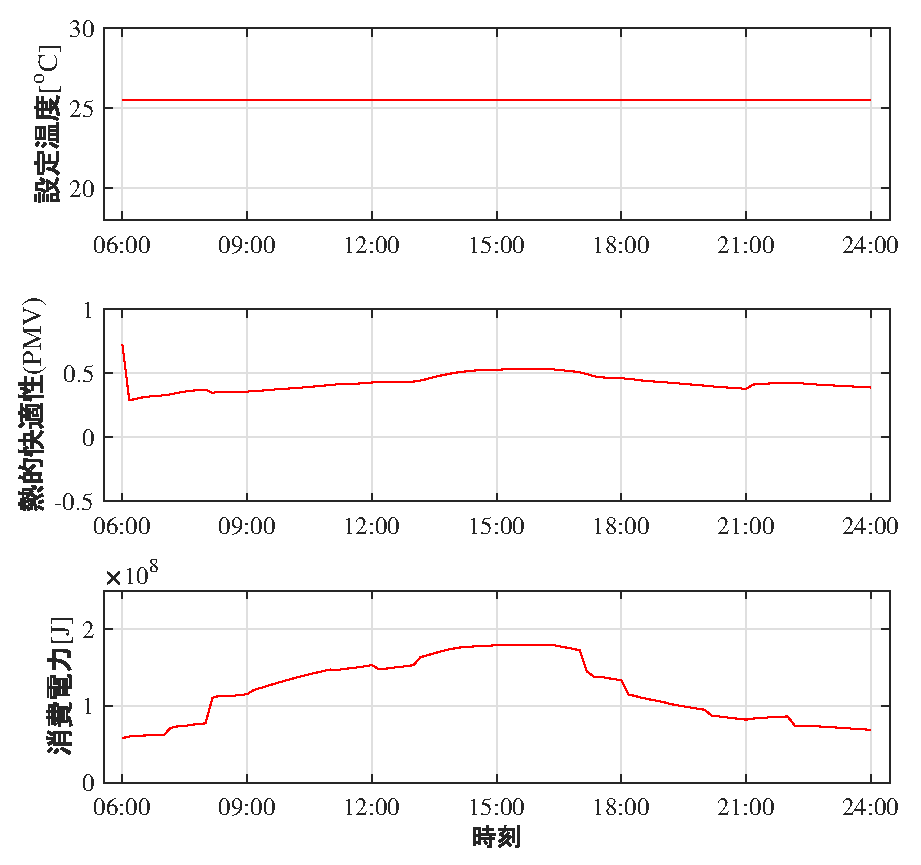
\includegraphics[width=1.0\textwidth,keepaspectratio=true]{fig/sim_result_schedule_e.eps}\\{スケジュール E (設定温度25.5[$^o$C])}
      \end{center}
    \end{minipage}
  \end{center}
  \vspace{2mm}
  \caption{従来システムで得られた設定温度スケジュールによる結果}
  \label{fig::sim_result_schedule_const}
\end{figure*}

\subsection{得られた設定温度スケジュールの時系列データ}\label{subsec::sim_schedule_timeseries}
\subsubsection{従来システムによる設定温度一定のスケジュールとの比較}
得られた設定温度スケジュールの時系列データについて議論する.\figref{fig::sim_result_pareto}において青い円で示した提案システムによる設定温度スケジュールA,B,Cについて,設定温度,室内快適性(PMV値),エネルギー消費量の時系列データを\figref{fig::sim_result_schedule}に示す.Aは最も快適だがエネルギー消費量が高いスケジュール,Cは最もエネルギー消費量が低いが快適性が低いスケジュール,Bは中間のバランスされたスケジュールとして\figref{fig::sim_result_pareto}から取り出した.また,従来システムによるDとEの時系列データを\figref{fig::sim_result_schedule_const}に示す.\figref{fig::sim_result_schedule}と\figref{fig::sim_result_schedule_const}において,室内快適性としてプロットした値は,範囲[-3, +3]のPMV値であり,\Eqref{eq::math_objective1}において第1目的関数の定式化に利用したPMV値の絶対値ではないことに注意されたい.そのため,ここでは,PMV値がゼロの場合に最も快適であり,マイナス値は寒さによって快適性が低下し,プラス値は暑さによって快適性が低下すると判断する.

まず,設定温度の時系列データについて,\figref{fig::sim_result_schedule_const}の従来システムが設定温度を一定にするのに対して,\figref{fig::sim_result_schedule}の提案システムは時刻の変化に伴って設定温度を動的に変更することがわかる.\figref{fig::sim_result_schedule_const}における従来システムの結果から,温度設定を一定にすると,15:00まで暑さによってPMV値が上昇し,同様にエネルギー消費量も上昇することがわかる.日中の外気温の上昇が,空調の熱源に生成する熱量の増加と効率の悪化を招き,エネルギー消費量が増加する.次に,室内快適性に関する第1目的関数値が同程度の提案システムによるスケジュールBと従来システムによるスケジュールDを比較すると,提案システムによるスケジュールBは,午前中に空調の設定温度を低下させ,15:00には設定温度を上昇させることで空調システムの負荷を低減させる.提案システムでは,設定温度の変更に伴い,熱源の生成する熱量が変化するため,空調システムのエネルギー消費量が変化する.これにより,午前中のエネルギー消費量は,設定温度を一定にする従来システムより高くなるが,15:00付近のエネルギー消費量は抑制される.その結果,\figref{fig::sim_result_pareto}に示したように,提案システムによるスケジュールBは,従来システムのスケジュールDより総エネルギー消費量を抑制できる.設定温度が一定の従来システムによるエネルギー消費量の変化は緩やかだが,設定温度を変更する提案システムの場合,設定温度を変更するタイミングでエネルギー消費量が急激に変化する傾向が見て取れる.しかし,提案システムは,このエネルギー消費量の急峻な増減が発生しても,一日の総エネルギー消費量としては低くなるスケジュールを生成している.また,従来システムによるスケジュールEについては,14:00~17:00の間に快適度が0.5を超過しており,制約条件\Eqref{eq::math_constraint_pmv}を満たしていないことが確認できる.

\figref{fig::sim_result_schedule}の室内快適性が低いスケジュールCは,PMV値が終日0.5に近い値で推移することがわかる.一方,\figref{fig::sim_result_schedule}の室内快適性が高いスケジュールAは,PMV値がゼロに近い値を維持することがわかる.スケジュールAは,14:00~16:00の外気温が高く,空調システムの効率が悪化してエネルギー消費量が上昇しやすい時間帯に温度設定を上げることにより,PMV値を上昇させてエネルギー消費量の増加を抑制することがわかる.

\begin{figure*}[htbp]
  \begin{center}
    \begin{minipage}{0.5\textwidth}
      \begin{center}
        \includegraphics[width=1.0\textwidth,keepaspectratio=true]{fig/sim_result_schedule_a_settemp_diff.eps}\\{(a) スケジュールAとその隣接解}
      \end{center}
    \end{minipage}
    \begin{minipage}{0.5\textwidth}
      \begin{center}
        \includegraphics[width=1.0\textwidth,keepaspectratio=true]{fig/sim_result_schedule_b_settemp_diff.eps}\\{(b) スケジュールBとその隣接解}
      \end{center}
    \end{minipage}
    \begin{minipage}{0.5\textwidth}
      \begin{center}
        \includegraphics[width=1.0\textwidth,keepaspectratio=true]{fig/sim_result_schedule_c_settemp_diff.eps}\\{(c) スケジュールCとその隣接解}
      \end{center}
    \end{minipage}
  \end{center}
  \vspace{-2mm}
  \caption{提案システムで得られた設定温度スケジュールの隣接解との差}
  \label{fig::sim_result_schedule_settemp_diff}
\end{figure*}

\subsubsection{獲得した設定温度スケジュールの特徴}
次に,提案システムで得られた設定温度スケジュールにどのようなパターンが存在するか分析する.\figref{fig::sim_result_schedule_settemp_diff}に,提案システムで得られた設定温度スケジュールA, B, Cと,その両隣に隣接したスケジュールA', A'', B', B'', C', C''のスケジュールを示す.\figref{fig::sim_result_schedule_settemp_diff}を見ると,設定温度スケジュールB,Cの近くには,概ねそれらのスケジュールに近い設計変数を持つ解しか存在しないのに対して,設定温度スケジュールAの近くにはAとは大きく異なる設計変数を持つ多様なスケジュールが存在する.
\red{定量的にこのスケジュールの多様性を評価するため,以下の\Eqref{eq::sim_mulltimodal_index}で定める$I_d$という評価尺度を導入する.
  \begin{eqnarray}
    I_d &= \frac{1}{100} \sum^{10}_{i=1} \sum^{10}_{j=1}(D_{i, j} - \bar{D})^{2}
    \label{eq::sim_mulltimodal_index}
  \end{eqnarray}
  ここで,$D_{i, j}$は,次の\Eqref{eq::sim_setpoint_distance}で定義される.この式は,ある設定温度スケジュール集合における$i$番目の設定温度$t_{set}^{i}(t)$と$j$番目の設定温度$t_{set}^{j}(t)$の各時刻の差の絶対値の総和であり,設計変数間の距離を表す.$\bar{D}$は,設定温度スケジュール集合の各設計変数間の距離の平均値である.
  \begin{eqnarray}
    D_{i, j} &= \sum^{n}_{t=1} |t_{set}^{i}(t) - t_{set}^{j}(t)|
    \label{eq::sim_setpoint_distance}
  \end{eqnarray}
  $I_d$はある設定温度スケジュール10個の設計変数間の距離の分散であり,この値が大きいほど設計変数が多様であることを示す.この多様性評価尺度$I_d$を提案システムで得られた設定温度スケジュールA, B, C付近の設計変数10個ずつを抽出してそれぞれに対して計算し正規化すると,設定温度スケジュールA付近では$I_d=1.0$であるのに対し,設定温度スケジュールB付近では$I_d=0.28$,設定温度スケジュールC付近では$I_d=0.1$となった.この結果から,定量的にも,設定温度スケジュールAの近くにはAとは異なる多様な設定温度スケジュールが存在し,設定温度スケジュールB,Cの近くにはそれらのスケジュールに近いスケジュールしか存在しないことがわかる.
}

この結果は,本章で扱う空調設定温度スケジュール最適化問題が,スケジュールA付近では離れた設計変数でも目的関数が良い点が存在する多峰性を持った関数であることを示唆している.これは,スケジュールCなどの制約条件に近いスケジュールの場合,設定温度を多少変更しただけで制約違反となってしまうことから,制約を満たしつつ目的関数を良くする設定温度スケジュールのパターンが制限されて一意に決まってくるのに対し,スケジュールA付近では多少の設定温度変更をしても制約違反とはなりにくく,様々な設定温度スケジュールのパターンによって目的関数を良くすることが可能であることが理由と考えられる.

異なる設計変数(スケジュール)が,同一もしくは類似した目的関数値を示す最適化問題をマルチモダル(Multimodal, 多峰性)最適化問題\cite{Tanabe20}という.目的関数空間におけるスケジュールAの周辺には,マルチモダル最適化の問題クラスに相当する傾向がみられることがわかった.提案システムは,このような多峰性を持つ問題であっても局所解に陥らず複数のパターンの中から他のパターンを優越する解を探索できているため,\figref{fig::sim_result_schedule_settemp_diff}(a)のように多様なパターンを解集合に含んでいるものと考える.
\red{これに対し,スケジュールB, Cの周辺は,似通った設計変数(スケジュール)が類似した目的関数値を示す.このような最適化問題をユニモダル(Unimodal, 単峰性)最適化問題と呼ぶ.空調設定温度スケジュール最適化問題は,目的関数空間のエリアによってマルチモダルおよびユニモダル最適化問題のそれぞれ異なる特性をもつ問題となっている.提案システムは,スケジュールAの近傍のマルチモダルな傾向の範囲だけではなく,スケジュールB, Cの近傍のユニモダルな傾向を持つ範囲であっても良好な解を探索できている.}

\red{
ここで,他のビルでも同様な傾向にあるか確認するため,以下の\figref{fig::sim_office_building_small}に示す小規模オフィスビルのシミュレーションモデルを用意し,提案システムによって空調設定温度スケジュールの多目的最適化を行った.この小規模オフィスビルモデルの対象は,地上1階建ての5つの部屋を持つ建物で,延床面積が464[$m^2$]である.床面積とフロアレイアウト以外のモデル設定は,\secref{sec::sim_model}で述べたオフィスビルモデルと同様である.また,最適化アルゴリズムおよび最適化部の設定は\secref{sec::sim_setting}と同様とした.
}
\begin{figure}[htbp]
  \begin{center}
    \vspace{-4mm}
    \includegraphics[width=0.6\linewidth, angle=90]{fig/sim_office_building_small.eps}
  \end{center}
  \vspace{-15mm}
  \caption{小規模オフィスビルモデルの外観}
  \label{fig::sim_office_building_small}
\end{figure}
\red{
  小規模オフィスビルシミュレーションモデルに対する多目的最適化を行い獲得した空調設定スケジュールを\figref{fig::sim_result_pareto_small}に示す.また,\figref{fig::sim_result_pareto_small}において,\figref{fig::sim_result_pareto}と同様に快適,不快,中間の室内快適性を持つスケジュールF, G, Hを抽出し青の円で示した.スケジュールF,G,Hそれぞれの付近の設計変数10個ずつに対して,スケジュールの多様性評価尺度$I_d$を計算し正規化すると,スケジュールF付近では$I_d=1.0$,スケジュールG付近では$I_d=0.57$,スケジュールH付近では$I_d=0.38$となった.この結果から,小規模オフィスビルでも中規模オフィスビルと同様に,目的関数空間に獲得されたスケジュールが多様であるエリアとそうではないエリアがある,マルチモダルおよびユニモダル最適化問題それぞれの異なる特性をもつ問題となっていることが確認できる.一方で,小規模オフィスビルの多目的最適化結果では,室内快適性に関する目的関数値が$0.24 \leq f_1 \leq 0.5$の解は得られていない.この理由は,ビル規模により快適性に関する制約条件\Eqref{eq::math_constraint_pmv}を満たすことの容易さに違いがあるためであると考える.規模の大きいビルでは,部屋の空間が広く,躯体も耐震性を配慮し強度の高いコンクリートが多分に使用されており,空調対象室の熱容量が大きい.そのため,設定温度変更に対して,室内温度・壁面温度が変化しにくく,快適性の変化は遅くなる.冷房条件では,空調負荷の高い日中帯は特に快適性の変化が遅くなるため,設計変数である設定温度を大きく変更しても制約の境界値を超過しにくい.結果として得られる温度スケジュールは多様性が高いものが多い傾向になる.一方で,小規模なビルでは空調対象室の熱容量が小さく,設定温度変更に対して快適性が急峻に変化する.空調機の特性によってはオーバーシュートやハンチングを起こすこともあるため,制約違反しやすい.このように制約を容易には満足できないため,制約の境界に近い$0.24 \leq f_1 \leq 0.5$の範囲では解を獲得できておらず,結果として得られる制約を満たした温度スケジュールは似通ったものが多い傾向になるものと考える.この小規模オフィスビル最適化問題は,最適化手法から見ると,制約を満たすことが難しいため探索により良好な解を獲得することが難しい問題であるといえる.しかし,このような難しさのある小規模オフィスビルの空調設定スケジュール最適化問題に対しても,提案システムは快適性とエネルギー消費量のトレードオフを近似する良好なパレート解候補を獲得できている.他の規模・フロアレイアウトや断熱材・空調システムなどの設定を持つオフィスビルにおいても,上述の中規模オフィスビル・小規模オフィスビルモデルと同様の問題クラスを持つとすれば,それらのオフィスビルにも提案システムが有効である可能性がある.
}

\begin{figure}[htbp]
  \begin{center}
    \includegraphics[width=0.7\linewidth]{fig/sim_result_pareto_small.eps}
  \end{center}
  \caption{小規模オフィスビルモデルのシミュレーション最適化の結果}
  \label{fig::sim_result_pareto_small}
\end{figure}

\subsection{計算時間}
本章の計算機実験の環境において,各粒子(スケジュール)を評価するEnergyPlusのシミュレーションには約40秒かかる.各評価シミュレーションを8並列で実行し,最適化の実行時間は37時間31分だった.このように,現在の計算機環境における提案システムでは,空調の設定温度スケジュールを得るために,約1.5日前に最適化を実行する必要がある.外気温予報などの入力データの精度は,予測時点が近いほど高まる.より精度が高い予報を含む入力データを利用するためには,より高速にシミュレーションを実行することが必要になる.このためには,シミュレーションの高速化やPCクラスタなどを導入した並列度の高い計算機環境を用いる手段などが考えられる.

\section{提案システム設計の妥当性検証}\label{sec::sim_valid}
提案システムの設計について,室内快適性に関する制約条件を設ける効果,$\epsilon$制約法による単一目的最適化との比較による多目的最適化する効果,異なる多目的進化計算法を用いたときの効果,OMOPSOによるアルゴリズム上の工夫の効果について議論する.

\subsection{制約条件を設ける効果}
\subsubsection{目的}
本論文の提案システムにおいて,室内快適性に関する制約条件\Eqref{eq::math_constraint_pmv}を設ける意義について検証する.一般的に,制約条件が,必ずしも満たす必要はないものの可能な限り満たしたいソフト制約の場合や,必ず満たさなければならないハード制約であっても実行可能解の獲得が困難な場合,最適化の過程で制約条件は考慮せず,獲得した解集合から制約条件を満たさない解を除去したり,制約条件に近い解を意思決定者に提示したりすることがある.この方法によって,最適化の過程で制約条件を考慮しなければ,より多様な解の探索が可能になるが,制約条件を考慮した最適化より実行可能解は得られにくくなる.本項では,制約条件を考慮する方法と考慮しない方法によって得られた解集合を比較することで,提案システムにおいて制約条件\Eqref{eq::math_constraint_pmv}を設ける意義と効果を明らかにする.

\begin{figure}[htbp]
  \begin{center}
    \includegraphics[width=0.7\linewidth]{fig/sim_result_pareto_cc.eps}
  \end{center}
  \caption{制約条件\Eqref{eq::math_constraint_pmv}の考慮の有無によって得られた解集合}
  \label{fig::sim_result_pareto_cc}
\end{figure}

\subsubsection{方法}
最適化の過程で,制約条件\Eqref{eq::math_constraint_pmv}を考慮する方法1,考慮しない方法2を比較する.方法1は,提案システムである.方法1と2は,ともに\tabref{tab::sim_param_omopso}に示すパラメータを用いる.


\subsubsection{結果}
得られた解集合の目的関数空間における分布を\figref{fig::sim_result_pareto_cc}に示す.この結果から,制約条件\Eqref{eq::math_constraint_pmv}を考慮しない方法2は,$f_1$値が高く快適性は悪いもののエネルギー消費量を抑制できるスケジュールを獲得できることがわかる.方法2が獲得した解集合の中で,制約条件\Eqref{eq::math_constraint_pmv}を満足する解集合に青い円で印をつけた.青い円の解集合は,最適化の過程で制約条件\Eqref{eq::math_constraint_pmv}を考慮する方法1による解集合と比較すると,エネルギー消費量が低くならないことがわかる.これは,第1目的関数における一日の室内快適性の平均値の最小化を試みても,方法2では,制約条件\Eqref{eq::math_constraint_pmv}における計測時刻ごとの室内快適性を満たしつつ第2目的関数であるエネルギー消費量が低いスケジュールを獲得することには困難があるといえる.提案システムである方法1は,制約条件\Eqref{eq::math_constraint_pmv}を設けることで,室内快適性の良好な解の獲得を促進し,その条件下でエネルギー消費量が低いスケジュールを獲得できたといえる.


\subsection{多目的最適化と$\epsilon$制約法による単一目的最適化}
\subsubsection{目的}
本論文の提案システムにおいて,室内快適性とエネルギー消費量を多目的に最適化する意義について検証する.多目的最適化する利点のひとつは,室内快適性とエネルギー消費量のトレードオフ関係をビル管理者に提示し,長期的なエネルギー消費計画と合わせて実行する設定温度スケジュールを意思決定させるためである.しかし,利用するスケジュールは,獲得した多様なスケジュール集合のうちの一つだけであり,利用しないスケジュールに探索計算コストをかけることになる.最適化に関する選好情報を利用し,単一目的最適化によって一つの解を求めることで,トレードオフになる多様なスケジュール集合は獲得しない手段も考えられる.本項では,本論文の空調最適化問題を単一目的最適化する方法と多目的最適化する方法を比較する.

\subsubsection{方法}
多目的最適化問題を単一目的最適化問題にして解く方法として,$\epsilon$制約法\cite{Haimes71}を取り上げる.$\epsilon$制約法は,複数の目的関数のうちいくつかに許容値を設けて制約条件とし,残りの目的関数を最適化する.本項では,次式による$\epsilon$制約法によって,多目的最適化問題である空調スケジュール最適化問題を単一目的最適化問題に変換する.
\begin{eqnarray}
  \begin{cases}
    \mbox{Minimize} \quad f_2(\vec{x})                  & \\
    \mbox{Subject\ to} \quad f_1(\vec{x}) \leq \epsilon & \\
  \end{cases}
\end{eqnarray}
すなわち,室内快適性に関する目的関数$f_1$に最大値$\epsilon$を与えることで制約条件にし,エネルギー消費量に関する目的関数$f_2$を最小化する単一目的最適化問題にする.本項では,$\epsilon = \{0.01, 0.1, 0.2, 0.3, 0.4\}$とし,5つの選好解を求めることにした.

単一目的最適化手法として,PSOと差分進化(Differential Evolution, DE) \cite{Price06}を用いた.
提案システムにおける多目的最適化のためのOMOPSOと比較するため,単一目的最適化のためのPSOには,ひとつの目的関数を扱うOMOPSOを用いる.単一目的最適化のため,リーダー粒子群$\mathcal{L}$およびアーカイブ粒子群$\mathcal{E}$のサイズを1にし,各世代で最良の目的関数値を持つ粒子をリーダーにすること以外は,提案システムにおける多目的最適化のためのOMOPSOと同じ設定を用いる.また,DEにおける解の生成法には,rand/1/binを用い,個体数50,総世代数500として,解の評価回数を等しくした.交叉率は$C_r=0.9$,スケーリング係数は$F=0.7$にした.単一目的最適化のPSOとDEの両方において,制約条件を伴う解の比較について,比較する2つの解が実行可能なら目的関数値$f_2$が良い方,片方が実行可能でもう片方が実行不能なら実行可能の方,2つの解が実行不可能なら$f_1$が$\epsilon$に近い方が良いと判断した.

ここで,本項で用いるPSOとDE,これらに利用するアルゴリズムのパラメータ,さらには単一目的化するための$\epsilon$制約法と制約条件の取り扱い方は,空調スケジュール最適化問題の単一目的最適化のために最良というわけではなく,単一目的最適化の手段の例として取り上げることに注意されたい.空調スケジュール最適化問題を含む実世界問題には,一つひとつの解の評価に時間を要するものがあり,最良の方法とパラメータを試行錯誤して見出すことは実質的に困難である.そのため,本項における単一目的最適化のためのPSOは,多目的最適化のためのOMOPSOと比較するために採用しており,DEも基礎的かつ一般的な方法とパラメータを採用している.

\begin{figure}[htbp]
  \begin{center}
    \includegraphics[width=0.7\linewidth]{fig/sim_result_pareto_multisingle.eps}
  \end{center}
  \caption{ 多目的最適化と$\epsilon$制約法に基づく単一目的最適化によって得られた解集合}
  \label{fig::sim_result_pareto_multisingle}
\end{figure}

\subsubsection{結果}
多目的最適化する提案システムを方法A,単一目的最適化する$\epsilon$制約法を組み込んだPSOを方法B,同じく$\epsilon$制約法を組み込んだDEを方法Cとし,得られた解集合を\figref{fig::sim_result_pareto_multisingle}に示す.方法Aは1回の実行結果,方法BとCは$\epsilon$が異なる5回の実行結果を示す.

まず,単一目的最適化する方法BとCを比較する.$\epsilon=0.4$を用いる場合,方法Bによる解は,方法Cによる解をパレート支配する.しかし,これら2つの解は,$f_1=0.4$近くまで到達できない.このように,$\epsilon$制約法において,$\epsilon$が大きい場合,$\epsilon$制約の境界近くに解を獲得しにくい傾向が見られた.$\epsilon=\{0.01,0.1\}$を用いる場合,方法Bの解は,方法Cの解より,それぞれ$f_1=\{0.01,0.1\}$への到達度が高い.しかし,方法Bの解は,エネルギー消費量$f_2$が方法Cの解より高く,方法Cの解にパレート支配される.

次に,多目的最適化する方法Aと単一目的最適化する方法B,Cを比較する.多目的最適化する方法Aが獲得した解集合は,単一目的最適化する方法BとCが獲得したそれぞれの解をパレート支配する解を内包することがわかる.方法AとBは,ともにPSOに基づく方法だが,異なる$\epsilon$を用いて単一目的最適化する方法Bを5回実行して得られた5つの解は,多目的最適化する方法Aを1回実行して得られた解にパレート支配される.
方法Aが多様な解を解集団中に保持して解の生成に活用することで,パレートフロントの特定部位を探索する方法BとCより良好な解を獲得したのだとすれば,多目的化法(Multi-objectivization) \cite{Knowles10}と呼ばれる方法において見られる効果と類似する可能性がある.

多目的最適化と単一目的最適化の良し悪しは簡単に議論できないが,上記のように,空調スケジュール最適化問題においては,本項で用いた$\epsilon$制約法を組み込んだ単一目的最適化するPSOとDEより,提案システムにおいて多目的最適化するOMOPSOが良好な解集合を1度の最適化で獲得する実験結果が得られた.

\subsection{多目的進化計算法の選択肢}\label{subsec::sim_algo}
\subsubsection{目的}
提案システムは,粒子群最適化に基づくOMOPSOを用いるが,多目的進化計算法には,他にも選択肢がある.本項では,異なる多目的進化計算法によって得られる解集合を比較する.

\subsubsection{方法}
OMOPSOと,\subsecref{subsec::NSGAII}で述べたNSGA-IIに加え,NSGA-III \cite{Deb14},MOEA/D-DE \cite{Li09}の4種類の多目的進化計算法を比較する.NSGA-III \cite{Deb14}は,NSGA-IIを基礎とする方法で,特に目的数が多い問題に有効である.NSGA-IIIは,目的関数空間にリファレンスライン群を用意し,NSGA-IIにおける混雑距離の代わりに解とリファレンスラインの直交距離を考慮して,目的関数空間における解の分布の均一性を高める.解の生成法として,NSGA-IIとNSGA-IIIには,Simulated Binary Crossover (SBX) \cite{Agrawal95}とPolynomial Mutation (PM) \cite{Deb96}を用いる.MOEA/D-DE \cite{Li09}は,MOEA/D \cite{Zhang07}を基礎とする方法である.MOEA/Dは,一様分布の重みベクトル群を生成し,各重みベクトルに基づくスカラー化関数群を同時に最適化することでパレートフロントの近似を試みる.解の生成法として,MOEA/DはSBXとPMを用いるが,MOEA/D-DEはDEとPMを用いる.また,MOEA/D-DEには,解の更新数に制限が設けられるなどの変更が導入されている.

\begin{table}[t]
  \begin{center}
    \caption{NSGA-IIとNSGA-IIIのパラメータ}
    \label{tab::sim_param_nsga}
    \small
    \begin{tabular}{c|cccc}
      \hline
      パラメータ           & 方法 / 値            \\
      \hline \hline
      交叉法               & SBX \cite{Agrawal95} \\
      SBX分布度 $\eta_{c}$ & 30                   \\
      交叉率 $p_{c}$       & 0.9                  \\
      突然変異法           & PM \cite{Deb96}      \\
      PM分布度$ \eta_{m}$  & 20                   \\
      突然変異率 $p_{m}$   & $1/n$                \\
      \hline
    \end{tabular}
  \end{center}
\end{table}

\begin{table}[t]
  \begin{center}
    \caption{MOEA/D-DEのパラメータ}
    \label{tab::sim_param_moead}
    \small
    \begin{tabular}{c|cccc}
      \hline
      パラメータ           & 方法 / 値                 \\
      \hline \hline
      交叉法               & rand/1/bin \cite{Price06} \\
      スケーリング係数$F$  & 0.5                       \\
      交叉率 $C_{r}$       & 1.0                       \\
      突然変異法           & PM \cite{Deb96}           \\
      PM分布度$ \eta_{m}$  & 20                        \\
      突然変異率 $p_{m}$   & $1/n$                     \\
      近傍サイズ$T$        & 5                         \\
      近傍選択確率$\delta$ & 0.9                       \\
      最大更新数$n_r$      & 2                         \\
      \hline
    \end{tabular}
  \end{center}
\end{table}

4種類のアルゴリズムについて,解集団サイズは50,総世代数500にした.OMOPSOのパラメータを\tabref{tab::sim_param_omopso}に示す.NSGA-IIとNSGA-IIIのパラメータを\tabref{tab::sim_param_nsga},MOEA/D-DEのパラメータを\tabref{tab::sim_param_moead}に示す.
それぞれのアルゴリズムの実装は,jMetal \cite{Nebro15}を一部改変して利用した.
\begin{comment}
本論文の空調最適化システムは,一つひとつの解の評価シミュレーションに時間を要するため,進化計算を複数回実行することは,システムの運用において実質的に不可能である.そのため,4種類のアルゴリズムは,同じ初期解集団から最適化を開始する同一条件下で,1回の実行結果を比較することとし,アルゴリズムの比較に関する以降の議論は,統計的な裏付けによるものではないことに注意されたい.
\end{comment}
\red{本実験では,それぞれのアルゴリズムについて初期値のシードを変更して20回の試行を行った.4種類の方法によって得られた解集合を定量的に評価するため,Hypervolume\cite{Zitzler99}(HV)を計算した.HVは,目的関数空間において,多目的最適化によって獲得した解集合が参照点との間に作る超体積を示す.獲得した非劣解集合の,パレートフロントへの収束性,多様性(目的関数空間上での広がり),分布の一様さ,解の数がそれぞれ良好な場合にHV値が大きくなる.そのためHVはパレートフロントの近似度合いを総合的に評価する指標として用いられている.今回は,4手法が全探索世代において評価した各目的関数値の最大値(最悪値)を参照点に設定した.また,全探索世代の最小値と最大値の範囲で各目的関数値を正規化したうえで,各世代の解集合のHV値を計算し各試行の平均値を求めた.}
\subsubsection{結果}
\begin{figure}[htbp]
  \begin{center}
    \includegraphics[width=0.7\linewidth]{fig/sim_result_hv_multi.eps}
  \end{center}
  \caption{4種類の多目的進化計算法による探索性能(Hypervolume値)の世代推移}
  \vspace{-6mm}
  \label{fig::sim_result_hv_multi}
\end{figure}

\begin{figure}[htbp]
  \begin{center}
    \includegraphics[width=0.7\linewidth]{fig/sim_result_pareto_multi.eps}
  \end{center}
  \caption{4種類の多目的進化計算法により獲得したパレートフロントの例}
  \vspace{-6mm}
  \label{fig::sim_result_pareto_multi}
\end{figure}

\red{
  4種類の手法でそれぞれ獲得した解集合の各世代のHVの平均値を\figref{fig::sim_result_hv_multi}に示す.本最適化問題においては,いずれの手法でも探索初期の35世代目までに実行可能解を発見することができ,その後HV値の高い良好な解の探索が進行した.最終世代では,4手法のうちOMOPSOが最も良いHVを示し,次いでNSGA-II, NSGA-III, MOEA/D-DEの順であった.MOEA/D-DEは探索初期の25世代程度は良い解を探索できているものの,その後の探索の進行が遅く,最終世代では最も悪いHV値となった.
  続いて,20回の試行のうち1回目の試行における,4種類の方法の最終世代に得られた解集合の例を\figref{fig::sim_result_pareto_multi}に示す.
}
最終世代では,いずれのアルゴリズムを用いても制約を満たし室内快適性とエネルギー消費量のトレードオフを表すスケジュール集合が獲得できていることがわかる.室内快適性$f_1$が0~0.2の範囲ではNSGA-II,0.2以上の範囲ではNSGA-IIIが,他の方法より良好な解集合を獲得したことがわかる.一方,OMOPSOは,室内快適性とエネルギー消費量のトレードオフを最も広範囲に表現する解集合を獲得したことがわかる.一方,MOEA/D-DEによる解集合は,目的関数空間の広域に分布するものの,他の方法による解集合と比較してパレートフロントに対する収束性が低いことがわかる.

\red{
  ここで,NSGA-II,NSGA-III,MOEA/D-DEが,OMOPSOに対して良好なHV値を獲得できなかった理由を考察する.
  まず,\figref{fig::sim_result_pareto_multi}のNSGA-III,MOEA/D-DEの分布を見ると,他の手法よりも解の間隔が広い事がわかる.これは,個体群の数が少ないことと,NSGA-IIIやMOEA/D-DEが用いる参照ベクトルの間隔が広く問題に対して偏りがあることが理由であると考えられる.このため均一で密度の高い解集合が獲得できておらず,高いHV値が得られていないものと考える.次に,NSGA-II,NSGA-IIIの解分布を見ると,他の手法に比べ$f_1$の快適性の値が大きい制約の境界に近い解が得られておらず,高いHV値の獲得が妨げられている.一方で,OMOPSOやMOEA/D-DEは,制約の境界付近の解を生成できており,広い分布の解が得られている.これは,NSGA-II,NSGA-IIIの解生成手法によるものと考える.OMOPSO,MOEA/D-DEでは,PSO・DEを用いた解生成を行っている.PSOは\subsecref{subsec::OMOPSO}に述べたように,個体群のうち良好な粒子方向のベクトルを足し合わせる交叉.DEはターゲットベクトルと変異ベクトルの交叉を用い,個体群の領域付近とその外側に確率的に子個体を生成する.一方,NSGA-II,NSGA-IIIで採用するSPXおよびPMは,\subsecref{subsec::ec}で述べたように,2つの親個体が持つ変数を中心とした各設計変数の周囲のみに子個体を生成するといった独特な解生成分布の特徴を持つ.このSBXとPMの持つ,生成される子個体の分布の特徴は,本問題の限られた領域の収束性の高い良好な解の発見には有効であったものの,制約付近の解の生成には有効ではなく,結果としてNSGA-II・NSGA-IIIは他手法のような広い範囲に分布する解集合の獲得ができなかったと考える.
}

\begin{comment}
\begin{table}[t]
  \begin{center}
    \caption{4種類の多目的進化計算法によるシミュレーション最適化で獲得した解集合のHypervolume(HV)値}
    \label{tab::sim_result_hv}
    \small
    \begin{tabular}{c|c|c|c|c}
      \hline
      手法 & NSGA-II & NSGA-III & MOEA/D-DE & OMOPSO \\
      \hline \hline
      HV値 & 0.621   & 0.628    & 0.589     & 0.643  \\
      \hline
    \end{tabular}
  \end{center}
\end{table}
\end{comment}

これらの結果から,提案システムで採用したOMOPSOは,他の多目的進化計算法と比較して高い性能を示し,室内快適性とエネルギー消費量のトレードオフを広域に近似可能で,ビル管理者に多様な設定温度スケジュール群を提示可能なアルゴリズムであるといえる.ただし,室内快適性が高い$f_1 \leq 0.2$の範囲ではNSGA-IIの性能が高いなど,提案システムにおける最適化アルゴリズムは代替可能であり,ビル管理者が求める性能によってアルゴリズムには選択の余地がある.

\subsection{OMOPSOによるアルゴリズム上の工夫の効果}
\subsubsection{目的}
本論文の提案システムにおいて,通常のMOPSOではなくOMOPSOを採用する意義について検証する.OMOPSOには\subsecref{subsec::OMOPSO}に記載したとおり,$\epsilon$-アーカイブという$\epsilon$優越でランク1となる解をサイズ制限無しに格納するアーカイブ,粒子の飛翔に用いるリーダー粒子群,一様突然変異・非一様突然変異・突然変異なしという3種の操作を加える突然変異,といったアルゴリズム上の工夫が行われている.これらの工夫はそれぞれ通常のMOPSOに対して解探索性能の向上を目的として導入したものであるが,これらの工夫が空調設定スケジュール最適化に対して有効でなければ,その工夫は必ずしも必要でないことになる.本項では,OMOPSOに対してこれらの工夫をそれぞれ無効化したアルゴリズムによって得られた解集合のHVを比較することで,提案システムにおいてOMOPSOを採用する意義と効果を明らかにする.

\subsubsection{方法}
OMOPSOを方法1, OMOPSOの工夫をそれぞれ無効化したアルゴリズム(方法2~4)を\tabref{tab::sim_cond_omopso_algo}の様に3つ定める.方法2は,$\epsilon$-アーカイブに対して最大アーカイブサイズを導入し,アーカイブサイズを超過する場合は混雑距離の短い解を除去する方法である.方法3は,リーダー粒子群を用いず,飛翔の際は$\epsilon$-アーカイブからバイナリトーナメントで選択した解をgBestとして用いる方法である.方法4は,突然変異を用いず,飛翔した粒子群をそのまま次世代の粒子群として用いる方法である.これらのアルゴリズムで空調設定スケジュール最適化を試行した結果を比較する.方法1~4は,ともに\tabref{tab::sim_param_omopso}に示すパラメータを用いる.ただし,方法2ではアーカイブサイズは100とする.また,本実験では,それぞれの方法1~4について初期値のシードを変更して20回の試行を行い,その平均のHVを比較する.

\begin{table}[ht]
  {\small
    \begin{center}
      \caption{OMOPSOのアルゴリズム上の工夫の検証方法}
      \label{tab::sim_cond_omopso_algo}
      \begin{tabular}{c|c|c|c|c}
        \hline
        方法  & 条件                 & アーカイブサイズ & リーダー粒子群 & 突然変異        \\
        \hline \hline
        方法1 & 通常のOMOPSO         & 制限なし         & あり           & 3種突然変異操作 \\
        方法2 & アーカイブサイズ制限 & 制限あり         & あり           & 3種突然変異操作 \\
        方法3 & リーダー粒子群不使用 & 制限なし         & なし           & 3種突然変異操作 \\
        方法4 & 突然変異なし         & 制限なし         & あり           & なし            \\
        \hline
      \end{tabular}
    \end{center}
  }
\end{table}

\subsubsection{結果}
20回試行によって得られた各世代の解集合のHVの平均値の推移を\figref{fig::sim_result_omopso_hv}に示す.本結果から,100世代までの探索初期では,方法2・方法4のアーカイブサイズに制限を設けた手法および突然変異操作を行わない手法が良いHV値を示すが,探索後期になると方法2, 方法3,方法4のHV値は方法1の通常のOMOPSO手法に劣った値を示すことがわかる.また,最終世代の解集合のHVの平均値を\tabref{tab::sim_result_omopso_hv}に示す.最終世代では方法1の通常のOMOPSOのHV値が他の方法のHV値よりも大きくなった.これらの結果から,方法2, 3, 4で示した,サイズ無制限の$\epsilon$-アーカイブ導入,リーダー粒子群を使用した飛翔,3種類の突然変異操作といった工夫が,本論文で取り上げた空調設定スケジュール最適化問題に対するOMOPSOの探索性能の向上に寄与していることが示された.
方法2,4が探索初期に良好な結果を示したのは,無制限のアーカイブサイズや突然変異操作がより多様な解探索を促進する手法であり,解集合の多様性よりもパレートフロントへの収束性が求められる探索初期には,これらの手法を含まないアルゴリズムのほうが早期に良好な解集合を探索できていたことが原因であると考えられる.ここから,OMOPSOのさらなる探索性能向上の工夫として,探索初期は$\epsilon$-アーカイブのサイズ制限を設けたり突然変異を行わずに探索し,ある解集合の分布が得られた段階でアーカイブサイズを拡張したり突然変異操作を行い,より多様な解の探索に切り替える手法が有効であると示唆される.


\begin{figure}[htbp]
  \begin{center}
    \includegraphics[width=0.7\linewidth]{fig/sim_result_omopso_hv.eps}
  \end{center}
  \caption{OMOPSOのアルゴリズム上の工夫によるHV値の世代推移の比較}
  \vspace{-6mm}
  \label{fig::sim_result_omopso_hv}
\end{figure}

\begin{table}[ht]
  {\small
    \begin{center}
      \caption{OMOPSOのアルゴリズム上の工夫によるHV値の比較}
      \label{tab::sim_result_omopso_hv}
      \begin{tabular}{c|c|c}
        \hline
        方法  & 条件                 & HV値   \\
        \hline \hline
        方法1 & 通常のOMOPSO         & 0.6554 \\
        方法2 & アーカイブサイズ制限 & 0.6546 \\
        方法3 & リーダー粒子群不使用 & 0.6474 \\
        方法4 & 突然変異なし         & 0.6451 \\
        \hline
      \end{tabular}
    \end{center}
  }
\end{table}


\section{結言}
本章では,オフィスビル全体の空調設定スケジュールを,シミュレーションを用いて最適化する手段について述べた.提案したシステムは,建築分野で用いられるシミュレータであるEnergyPlusを用いたシミュレーションにより,目的関数および制約を計算する.シミュレータに対してOMOPSOアルゴリズムを適用して,空調設定スケジュールの非劣解集合を探索した.実験結果により室内快適性とエネルギー消費量の双方が良好なスケジュールの非劣解集合を獲得できることを示した.
また,本研究で導入した制約条件が,快適性の良好なスケジュール獲得に寄与することを示した.さらに,$\epsilon$制約法をPSOとDEに組み込んだ単一目的最適化手法より,多目的最適化する手法のほうが良好なスケジュールを獲得できることを示した.加えて,代表的な多目的最適化手法であるNSGA-II,NSGA-III,MOEA/D-DEと比較して,OMOPSOは,最も広範囲に広がり,良好なHypervolume値を示す非劣解集合を獲得できることを示した.そして,OMOPSOが従来のMOPSOに対して持つアルゴリズム上の工夫が,本シミュレーション最適化の探索性能向上に寄与していることを示した.
本章で述べた試みにより,ビル全体の空調設定スケジュール最適化のために,シミュレーションを利用する方法の実現可能性が示された.

一方で,シミュレーションに基づく最適化には時間がかかる.1つのスケジュールの評価に約40秒かかり,一日の設定温度スケジュールを得るための最適化の全工程には約37.5時間かかる.これが原因となり,2つの問題が生じる.

1つ目は,精度の低い気象予報が最適化に悪影響を与えることである.シミュレータには,外気温予報を$\mathcal{A}$として入力する.予報と実際には差異が生じるが,直近の予報ほど正確性が高い\cite{JMA19}.本章の最適化システムは,最適化に約37.5時間かかるため,空調の運転を開始する一日半前の外気温予報を利用せざるを得ない.予報と実際の気象に差異が生じると,得られた空調設定スケジュールが最適にならないリスクがある.外気温の予報と実際の差異を考慮できれば,この問題を軽減できる可能性がある.この問題には,次の\chapref{chap::robust}で述べるロバスト最適化法で対処する.

2つ目は,進化計算で最適化するために十分な評価回数を実行できない恐れがあることである.進化計算は,膨大な解を生成しながら解評価をもとに探索を行い最適化する.1つの解の評価に時間がかかる場合,総評価回数を少なくせざるを得ず,最適化結果に影響を与える.この問題への対処法としてEnergyPlusのシミュレータの出力をもとに,エネルギー消費量・室内快適性のみを簡易に推定することで進化計算を加速するサロゲート最適化がある.本手法は,\chapref{chap::surrogate}で詳しく述べる.

\chapter{ロバスト最適化}
\label{chap::robust}

\hspace{1zw}本章では,外気温の予報と実際の差異に対処するためのロバスト最適化の試みについて述べる.

\section{概要}
最適化システムの構成を\figref{fig::robust_system}に示す.前章のシステムと同様に,評価部では,EnergyPlusシミュレーションを用いる.前章のシステムとの違いは,目的関数である.外気温予報に誤差がない場合の室内快適性に関する第1目的関数$f_1$, エネルギー消費量に関する第2目的関数$f_2$に加え,外気温予報に誤差がある場合の快適性の変動幅に関する第3目的関数$f_3$とエネルギー消費量の変動幅に関する第4目的関数$f_4$を考慮する.これら4つの目的関数を最適化することによって,外気温予報の誤差にロバストな空調設定スケジュールを得る.

\begin{figure*}[t]
    \begin{center}
        \includegraphics[width=1.1\linewidth]{fig/robust_system.eps}
    \end{center}
    \caption{ロバスト最適化システム}
    \label{fig::robust_system}
\end{figure*}

\section{ロバスト最適化における解評価}
\subsection{過去の予報・実績値に基づくシミュレーション用気温設計}\label{subsec::robust_airtemp}
\subsubsection{過去の気温予報実績の調査}
空調スケジュールの最適化における気温予報誤差を考慮するために,過去の気温実績値および気温予報値を利用する.日本国気象庁の提供する時系列気象予報データ\cite{JMAforecast}および実績データ\cite{JMAactual}を用いる.今回は夏期を対象としており2018年6月~9月のデータを使用して誤差を評価した.気温予報発表時刻は5:00であり,毎日6:00~24:00の予報気温と実際の気温を比較する.\figref{fig::robust_temperror_histogram}に各時刻の予報誤差レベル(実際の気温-予報気温)のヒストグラムを示す.色の違いは時刻の違いを表す.また,\tabref{tab::robust_temperror_statistics}に予報誤差の平均と標準偏差(SD: Standard Deviation)を示す.これらの結果から,各時刻における気温予報誤差は正規分布の傾向にあることがわかる.
一方で,気温予報誤差は各時刻で独立に正規分布で出現するわけではなく,時刻間で依存する傾向があることが知られている.\figref{fig::robust_boxplot}に,(a)最高気温予報が上方誤差を含む日の各時刻における気温予報誤差,(b)最高気温予報が下方誤差を含む日の気温予報誤差の箱ひげ図を示す.この結果から,最高気温予報が上方誤差を含む日は各時刻の誤差も上方に,下方誤差を含む日は各時刻の誤差も下方に出現する傾向がある.そこで,本研究では,\tabref{tab::robust_temperror_statistics}に示すような各時刻$t$における平均$μ_t$・標準偏差$σ_t$を有する正規分布が,上方の予報誤差を生じる場合および下方の予報誤差を生じる場合の2つを取り扱う.


\begin{figure}[t]
    \centerline{\includegraphics[scale=0.7]{fig/robust_temperror_histogram.eps}}
    \caption{外気温予報誤差のヒストグラム(2018年6~9月, 気象庁発表データ\cite{JMAforecast, JMAactual}をもとに作成)}
    \label{fig::robust_temperror_histogram}
\end{figure}

\begin{figure*}[htbp]
    \begin{center}
        \begin{minipage}{0.7\textwidth}
            \begin{center}
                \includegraphics[width=1\textwidth,keepaspectratio=true]{fig/robust_boxplot_upward.eps}\\{\small (a)最高気温予報に上方誤差を含む場合}
            \end{center}
        \end{minipage}
        \\
        \begin{minipage}{0.7\textwidth}
            \begin{center}
                \includegraphics[width=1\textwidth,keepaspectratio=true]{fig/robust_boxplot_downward.eps}\\{\small (b)最高気温予報に下方誤差を含む場合}
            \end{center}
        \end{minipage}
        \vspace{-1mm}
        \caption{外気温予報誤差の箱ひげ図}
        \label{fig::robust_boxplot}
    \end{center}
\end{figure*}

\begin{table}
    \caption{気温予報誤差の統計値}
    \label{tab::robust_temperror_statistics}
    \scalebox{0.85}[0.85]{
        \begin{tabular}{c|c|c|c|c|c|c|c|c}
            \hline
            \textbf{時刻} $t$       & \textbf{6:00} & \textbf{9:00} & \textbf{12:00} & \textbf{15:00} & \textbf{18:00} & \textbf{21:00} & \textbf{24:00} & \textbf{全体} \\
            \hline
            \hline
            平均値$\mu_t$           & -0.0554       & 0.0317        & 0.126          & -0.0448        & -0.134         & -0.08          & -0.00488       & -0.140        \\
            \hline
            標準偏差(SD) $\sigma_t$ & 0.654         & 1.20          & 1.35           & 1.02           & 0.791          & 1.10           & 1.23           & 1.32          \\
            \hline
        \end{tabular}}
\end{table}

\subsubsection{シミュレーション用外気温の設計}
本研究では,気温予報値を$\hat{\mathcal{A}}=\{\hat{a}_{5:00},\hat{a}_{6:00},\dotsc,$ $\hat{a}_{24:00}\}$で表す.ここで$\hat{a}_{t}$は時刻$t\in \{5:00,6:00,\dotsc,24:00\}$における予報気温である.例えば,$\hat{a}_{12:00}=32.0$ [${}^\circ$C]という予報値を示す.気温予報は毎日5:00に発表され,空調設定スケジュールは予報に基づいて最適化される.ビルシミュレータの入力として,気温予報誤差を考慮しない気温を$\mathcal{A}=\{a_{5:00},a_{6:00},\dotsc,$ $a_{24:00}\}$と表す.ここで$a_{t}$は$a_{t}=\hat{a}_{t}+\mu_t$によって得られる時刻$t$における修正された気温である.また,本研究で考慮する気温予報誤差の分散は,多くの誤差発生ケースに対応できるよう$\pm 2\sigma$とする.上方誤差分布を含む気温を$\mathcal{A}^{+2\sigma}=\{a^{+2\sigma}_{5:00},a^{+2\sigma}_{6:00},\dotsc,a^{+2\sigma}_{24:00}\}$,下方誤差分布を含む気温を$\mathcal{A}^{-2\sigma}=\{a^{-2\sigma}_{5:00},a^{-2\sigma}_{6:00},\dotsc,a^{-2\sigma} _{24:00}\}$で表す.時刻$t$における上方予報誤差分布を含む気温$a^{+2\sigma}_t$を以下の式で定義する.

\begin{align}
    \label{eq::robust_airtemp_upward}
    a^{+2\sigma}_t=a_t+2\sigma_t
\end{align}

ここで$\sigma_t$は\tabref{tab::robust_temperror_statistics}における外気温予報誤差の時刻$t$におけるSD値である.同様に,下方予報誤差を含む気温$a^{-2\sigma}_t$を以下の式で定義する.
\begin{align}
    \label{eq:atm2s}
    a^{-2\sigma}_t=a_t-2\sigma_t
\end{align}
\figref{fig::robust_system}で示したように,シミュレーションにおける予報誤差を含まない気温$\mathcal{A}$は,人の室内快適性レベル$f_1$とエネルギー消費量$f_2$の算出に使用される.予報誤差を含む気温$\mathcal{A}^{+2\sigma}$, $\mathcal{A}^{-2\sigma}$は室内快適性とエネルギー消費量のロバスト性を示す目的関数$f_3$, $f_4$の計算に使用される.これらの目的関数の詳細は\secref{sec::robust_objectives}で解説する.

\subsection{設計変数}
本章において,設計変数は\chapref{chap::sim}と同様に,空調設定温度スケジュール$t_{set}(t)$を最適化することとする. 本章では,分割時間間隔$T_s=1$[hour]として,設定可能時刻集合を$\mathcal{T}_{set}=\{6:00, 7:00,\dots, 24:00\}$とする.また設定温度スケジュールを設計変数で表す方法として,\Eqref{eq::sim_variable_diff}を用いる.

\subsection{目的関数}\label{sec::robust_objectives}
本章では,外気温予報に誤差がない場合の室内快適性に関する第1目的関数$f_1$, エネルギー消費量に関する第2目的関数$f_2$に加え,外気温予報に誤差がある場合の快適性の変動幅に関する第3目的関数$f_3$とエネルギー消費量の変動幅に関する第4目的関数$f_4$を考慮する.
\subsubsection{予報誤差のない場合の快適性・エネルギー消費量の評価}
室内快適性に関する第1目的関数$f_1$, エネルギー消費量に関する第2目的関数$f_2$については,\chapref{chap::sim}と同様に予報誤差を考慮しない気温$\mathcal{A}$を用いて,\Eqref{eq::sim_pmv},\eqref{eq::sim_asee}で算出する.

\subsubsection{気温予報誤差がある場合のロバストネスの評価}
目的関数値$f_1$, $f_2$は外気温$\mathcal{A}$の影響を受ける.\subsecref{subsec::robust_airtemp}で述べたように,$f_1$, $f_2$で入力されている$\mathcal{A}$は予報誤差を考慮していない.$\mathcal{A}$と実際の気温に差異がある場合,$\mathcal{A}$に対して最適化された空調スケジュール$\vec{x}$は最適解ではないことがある.快適性レベル$f_1$とエネルギー消費量$f_2$の空調予報誤差の影響を低減するために,本研究では,$f_1$と$f_2$に加えて2つの目的関数の不確実性を考慮する.
第三の目的関数は,上方と下方の予報誤差が発生した場合のビルシミュレーション結果における,予報誤差がない場合との室内快適性レベルの差の最小化とし,以下の目的関数で定式化する.
\begin{align}
    \text{Minimize}~f_3(\vec{x}) & = \max \{|f_1(\vec{x}, \mathcal{A}^{+2\sigma})-f_1(\vec{x}, \mathcal{A})|, |f_1(\vec{x}, \mathcal{A}^{-2\sigma})-f_1(\vec{x}, \mathcal{A})|\}
    \label{eq::robust_objective3}
\end{align}
ここで,$f_1(\vec{x}, \mathcal{A})$は外気温予報が$\mathcal{A}$の場合の室内快適性に関する第1目的関数,$\mathcal{A}^{+2\sigma}$,$\mathcal{A}^{-2\sigma}$は,\subsecref{subsec::robust_airtemp}で述べた上方および下方の誤差分布を含む気温推移である.

同様に,第四の目的関数は,上方と下方の予報誤差が発生した場合のビルシミュレーション結果における,予報誤差がない場合とのエネルギー消費量の差の最小化とし,以下の目的関数で定式化する.

\begin{align}
    \text{Minimize}~f_4(\vec{x}) & = \max \{|f_2(\vec{x}, \mathcal{A}^{+2\sigma})-f_2(\vec{x}, \mathcal{A})|, |f_2(\vec{x}, \mathcal{A}^{-2\sigma})-f_2(\vec{x}, \mathcal{A})|\}
    \label{eq::robust_objective4}
\end{align}

\section{実験内容}
本章では,天気予報誤差によるロバスト性を考慮することの有効性を検証するために2つの手法を比較する.1つめの方法は気温予報誤差を考慮せずに2つの目的関数値$f_1$, $f_2$を最適化する.2つめの方法は,気温予報誤差を考慮して4つの目的関数$f_1$, $f_2$, $f_3$, $f_4$を最適化する.最適化には\subsecref{subsec::OMOPSO}で述べたOMOPSOによって探索する.

\subsubsection{評価シミュレーション部の設定}
本章ではシミュレーションの対象日を\secref{sec::sim_setting}と同様に2006年8月21日の拡張アメダスデータを用い,同じ空調運転モードと設定温度の上下限値を用いる.\figref{fig::robust_outside_temp}に予報誤差を考慮しない気温$\mathcal{A}$および上方・下方の予報誤差を考慮した気温$\mathcal{A}^{+2\sigma}$,$\mathcal{A}^{-2\sigma}$の1日の推移を示す.

\begin{figure}[ht]
    \begin{center}
        \includegraphics[width=0.7\linewidth]{fig/robust_outside_temp.eps}
    \end{center}
    \caption{シミュレーションに用いた外気温度の推移}
    \label{fig::robust_outside_temp}
\end{figure}

\subsubsection{最適化部の設定}
OMOPSOで用いるパラメータを\tabref{tab::robust_param_omopso}に示す.EnergyPlusシミュレータの実行プログラムとOMOPSOアルゴリズムは\secref{sec::sim_setting}同様Javaで実装した.また,計算の実行にはPCクラスタ(15PC,Windows Server 2012 R2 64ビット,AMD Ryzen7 1800X 3.6GHz, 16GB RAM)を用いた.

\begin{table}[ht]
    {\small
        \begin{center}
            \caption{OMOPSOのパラメータ}
            \label{tab::robust_param_omopso}
            \begin{tabular}{c|cccc}
                \hline
                パラメータ                             & 方法 / 値              \\
                \hline \hline
                ベース粒子群サイズ $N^{\mathcal{P}}$   & 30                     \\
                リーダー粒子群サイズ $N^{\mathcal{L}}$ & 100                    \\
                アーカイブ粒子群サイズ                 & 制限なし               \\
                総世代数 $g_{max}$                     & 500                    \\
                変数長 $n$                             & 19                     \\
                突然変異率 $p_m$                       & $1/n$                  \\
                重み $w$                               & [$0.1, 0.5$)の一様乱数 \\
                重み $c_1, c_2$                        & [$1.5, 2.0$)の一様乱数 \\
                非一様突然変異の係数 $b$               & 5 \cite{Esquivel03}    \\
                $\epsilon$-dominanceの係数$\epsilon$   & 0.0075                 \\
                \hline
            \end{tabular}
        \end{center}
    }
\end{table}

\begin{figure}[htbp]
    \begin{center}
        \includegraphics[width=0.7\columnwidth,keepaspectratio=true]{fig/robust_result_pareto_f1f2.eps}\\
        {(a) $f_1$-$f_2$目的関数空間}
    \end{center}
    \begin{center}
        \includegraphics[width=0.7\columnwidth,keepaspectratio=true]{fig/robust_result_pareto_f3f4.eps}\\
        {(b) $f_3$-$f_4$目的関数空間}
    \end{center}
    \caption{ロバスト最適化の結果}
    \label{fig::robust_result_pareto}
\end{figure}

\begin{figure*}[htbp]
    \begin{center}
        \begin{minipage}{.7\textwidth}
            \begin{center}
                \includegraphics[width=1\textwidth,keepaspectratio=true]{fig/robust_result_schedule_accumulated_comfort.eps}\\\vspace{0.1cm}
                {(a) $f_3$(室内快適性の変動量)の積算値}
            \end{center}
        \end{minipage}
        \begin{minipage}{.7\textwidth}
            \begin{center}
                \includegraphics[width=1\textwidth,keepaspectratio=true]{fig/robust_result_schedule_accumulated_power.eps}\\\vspace{0.1cm}
                {(b) $f_4$(エネルギー消費の変動量)の積算値}
            \end{center}
        \end{minipage}
        \vspace{-0.0cm}
        \caption{外気温予報が誤差を含む$\mathcal{A}^{+2\sigma}$と$\mathcal{A}^{-2\sigma}$であった場合の,$f_3$と$f_4$のロバストネス指標値の時間ごとの積算値}
        \label{fig::robust_result_schedule_accumulated}
    \end{center}
\end{figure*}

\section{実験結果と考察}
\subsection{得られた設定温度スケジュール集合の目的関数値}
まず,ロバスト性を考慮せず目的関数値$f_1$と$f_2$を最適化する方法,ロバスト性を考慮して目的関数$f_1$, $f_2$, $f_3$, $f_4$を最適化する方法を比較する.得られた設定温度スケジュール集合を$f_1$, $f_2$目的関数空間上にプロットした結果を\figref{fig::robust_result_pareto} {\bf (a)}に示す.赤点が$f_1$と$f_2$のみを考慮して最適化した結果,黒点がロバスト性に関する目的関数$f_3$と$f_4$も考慮した結果である.$f_1$, $f_2$はそれぞれ小さいほど室内快適性レベル,エネルギー消費量が少なく良好なスケジュールである.

結果から,提案システムにより得られたすべてのスケジュールの室内快適性レベル$f_1$は0.5未満であり,\Eqref{eq::math_constraint_pmv}を満たして実行可能なスケジュールが得られていることがわかる.ロバスト性を考慮しない赤点の結果は30個に対して,ロバスト性を考慮した黒点の結果は880個の解を獲得した.4目的を考慮すると,2目的よりも個々の解の優劣をつけることが困難となり,非劣解となる解が多く発生したためと考える.また,$f_1$, $f_2$を考慮するだけで赤のスケジュールが得られるが,4目的の場合ロバスト性という別の目的関数$f_3$, $f_4$も考慮するため,2目的で探索したほうが目的関数$f_1$,$f_2$でよい値の解の割合が多い.\red{ここで,ロバスト性を考慮しない赤点の2目的最適化とロバスト性を考慮した黒点で示した4目的最適化それぞれで得られたスケジュール集合について,2つの目的関数$f_1$, $f_2$に対するHypervolume値を計算し正規化した結果を\tabref{tab::robust_result_hv}に示す.この結果から,ロバスト性を考慮した4目的最適化の手法では$f_1$, $f_2$目的関数空間で良い解の割合は少ないものの,$f_1$, $f_2$目的関数空間においてもロバスト性を考慮しない2目的最適化と同等かそれより良い解を含んでいる事がわかる.}


\begin{table}[t]
    \begin{center}
        \caption{ロバスト性を考慮しない2目的最適化とロバスト性を考慮した4目的最適化それぞれで獲得した解集合のHypervolume(HV)値}
        \label{tab::robust_result_hv}
        \small
        \begin{tabular}{c|c|c}
            \hline
            手法 & ロバスト性を考慮しない手法(2目的) & ロバスト性を考慮した手法(4目的) \\
            \hline \hline
            HV値 & 0.813                             & 0.866                           \\
            \hline
        \end{tabular}
    \end{center}
\end{table}

同様に,得られた設定温度スケジュール集合を$f_3$, $f_4$目的関数空間上にプロットした結果を\figref{fig::robust_result_pareto} {\bf (b)}に示す.$f_3$と$f_4$は,それぞれ小さいほど外気温の予報誤差による変動を低減できるロバストなスケジュールである.結果から,$f_3$, $f_4$を考慮した黒の点は,赤の点よりも値が小さく良いロバストネスの解を含み,多くの赤の点は,$f_3$, $f_4$の2次元の目的関数空間上で黒の点に優越される.\red{これらの結果から,黒の点で示したロバスト性を考慮した4目的最適化で獲得した設定温度スケジュール集合は,$f_1$, $f_2$目的関数でロバスト性を考慮しない赤の点と同等の解を選択肢として含みつつ,$f_3$, $f_4$で良好であるロバスト性な解を多数探索できていることが分かる.}気温予報はしばしば誤差を含むため,気温予報誤差におけるロバストネスを考慮した空調スケジュールはビル運用において実用的であるといえる.

\red{
    さらに,\figref{fig::robust_result_pareto} {\bf (a)}において4目的最適化で得られた解集合の分布について考察する.4目的最適化によって獲得した解集合は,$f_1 \leq 0.25$の範囲では幅広い範囲に分布しているが,$f_1 \geq 0.25$の範囲では得られている解分布の範囲は狭くなり2目的最適化と同様の解しか得られなくなる.これは,\subsecref{subsec::sim_schedule_timeseries}で述べたような,空調設定スケジュール最適化問題の部分的に多峰性を持つという問題の特徴によるものであると考える.本問題は$f_1$が小さい範囲では多峰性を持ち,異なる設計変数でも類似した目的関数値が得られるため,$f_1$は同様の値でありながらエネルギー消費量$f_2$が悪い値でロバスト性の高い解など,多数存在する多様な解候補を探索できている.これに対し.$f_1$が大きい範囲では制約違反になりやすく設計変数のパターンは類似したものが多くなり,解候補の多様性は低く2目的最適化と同様の値の解しか探索できない.このような傾向があるため,4目的最適化で得られた解集合の分布が$f_1$の範囲によって異なる傾向を持っていると考える.この結果は,上述のようにある最適化問題の各目的関数のロバスト性を目的関数として加えて探索を行うことで,問題の特徴を目的関数空間上の分布として可視化し推測することが可能であることを示唆している.これは,対象とする実世界の最適化問題の難易度を理解するための手法として有効な方法であることが考えられる.
}

\subsection{空調設定スケジュールの時系列分析}
\figref{fig::robust_result_pareto}から2つの得られたスケジュールを抽出し,時系列データの分析を行った.ここでは,ロバストネスを考慮しない2目的最適化の結果から得られたスケジュール$B$と,ロバストネスを考慮した4目的最適化の結果から得られたスケジュール$B'$について着目した.\figref{fig::robust_result_pareto} {\bf (a)}に示すように,$B$と$B’$は$f_1$-$f_2$目的関数空間において近くに位置しているが,一方で\figref{fig::robust_result_pareto} {\bf (b)}に示すように,$f_3$-$f_4$目的関数空間においては$B'$は$B$を優越している.\figref{fig::robust_result_schedule_accumulated} {\bf (a), (b)}に,$B$および$B'$の$f_3$, $f_4$の目的関数値の時間による積算値を示す.両方の図において,小さい値が快適度合いとエネルギー消費量においてロバストであることを示す.この結果から,4目的最適化によって得られた$B'$はロバスト性を考慮していない2目的最適化から得られた$B$に対して$f_3$, $f_4$の積算値が低く,ロバスト性を考慮した提案手法は予報温度誤差による快適度とエネルギー消費量の変動の小さい空調設定温度スケジュールが得られていることがわかる.ロバストな空調設定スケジュールは計画変更の回数を削減でき,月次・年次の電力消費計画を策定するビル管理者にとって実用的である.

\begin{figure*}[htbp]
    \begin{center}
        \begin{minipage}{0.5\textwidth}
            \begin{center}
                \includegraphics[width=1\textwidth,keepaspectratio=true]{fig/robust_result_schedule_2obj_setting.eps}\\(a) 空調設定温度スケジュール
            \end{center}
        \end{minipage}
        \begin{minipage}{0.5\textwidth}
            \begin{center}
                \includegraphics[width=1\textwidth,keepaspectratio=true]{fig/robust_result_schedule_2obj_comfort.eps}\\(b) 室内快適性レベル
            \end{center}
        \end{minipage}
        \begin{minipage}{0.5\textwidth}
            \begin{center}
                \includegraphics[width=1\textwidth,keepaspectratio=true]{fig/robust_result_schedule_2obj_power.eps}\\(c) エネルギー消費量
            \end{center}
        \end{minipage}
        \caption{ロバスト性を考慮しない2目的最適化で獲得した空調設定スケジュール$B$の時系列データ}
        \label{fig::robust_result_schedule_2obj}
    \end{center}
\end{figure*}

\begin{figure*}[htbp]
    \begin{center}
        \begin{minipage}{0.5\textwidth}
            \begin{center}
                \includegraphics[width=1\textwidth,keepaspectratio=true]{fig/robust_result_schedule_4obj_setting.eps}\\(a)空調設定温度スケジュール
            \end{center}
        \end{minipage}
        \begin{minipage}{0.5\textwidth}
            \begin{center}
                \includegraphics[width=1\textwidth,keepaspectratio=true]{fig/robust_result_schedule_4obj_comfort.eps}\\(b) 室内快適性レベル
            \end{center}
        \end{minipage}
        \begin{minipage}{0.5\textwidth}
            \begin{center}
                \includegraphics[width=1\textwidth,keepaspectratio=true]{fig/robust_result_schedule_4obj_power.eps}\\(c) エネルギー消費量
            \end{center}
        \end{minipage}
        \caption{ロバスト性を考慮した4目的最適化で獲得した空調設定スケジュール$B'$の時系列データ}
        \label{fig::robust_result_schedule_4obj}
    \end{center}
\end{figure*}

\figref{fig::robust_result_schedule_2obj}と\figref{fig::robust_result_schedule_4obj}に,ロバスト性を考慮していない空調設定スケジュール$B$とロバスト性を考慮した$B’$のスケジュールの,空調設定温度,室内快適性レベル,エネルギー消費量の時系列データをそれぞれ示す.室内快適性およびエネルギー消費量の結果では,緑の線が気温誤差のない場合,赤の線が上方の気温予報誤差がある場合,青の線が下方の気温予報誤差がある場合を示す.\figref{fig::robust_result_schedule_2obj} {\bf (a)}および\figref{fig::robust_result_schedule_4obj} {\bf (a)}から,従来の空調システムは設定温度を1日にわたって一定に保持するのに対し,提案システムは空調設定温度を時間毎に動的に変更していることがわかる.\figref{fig::robust_result_schedule_2obj} {\bf (a)}はロバスト性を考慮しない2目的最適化により得た解$B$のスケジュールであり,設定温度変更幅が小さめである.そのために,\figref{fig::robust_result_schedule_2obj} {\bf (c)}に示すように9:00~13:00と16:00~18:00あたりのエネルギー消費量が気温予報誤差に従って大きく変化してしまっている.
一方,\figref{fig::robust_result_schedule_4obj} {\bf (a)}は不確実性を考慮した4目的最適化で得られた結果$B'$のスケジュールであり,2目的の$B$に比べ設定の変動幅が大きい.結果として,ロバストな解$B'$は,ロバストでない$B$と$f_1$, $f_2$は同程度の値であるにもかかわらず,室内快適性$f_3$およびエネルギー消費量$f_4$の気象予報誤差による変動を低減できている.また,ロバストな解$B'$は昼間の12:00~13:00の時間帯に温度を低く保つことで,効率的に室温を冷やすように運転できている.
ロバスト性を考慮していない温度設定$B$は,気温予報誤差がある場合エネルギー消費量が149[kWh]増加するが,一方ロバスト性を考慮した温度設定$B'$は147[kWh]で済み,気象予報誤差によるエネルギー消費量の増加を1.2\%低減することができている.気温予報はしばしば誤差を含むため,ロバストな空調設定温度スケジュールはビル運用に実用的である.これは,提案した4目的最適化システムがより多様な解を獲得し,ビル管理者に対し提供でき,有用であることを示す.

\subsection{$\pm 2\sigma$以外の気温予報誤差に対するロバスト性の評価}
\subsubsection{目的}
本章で提案した手法では,本章で想定した,各時刻$t$において上方もしくは下方に$2\sigma$の気温予報誤差が発生した場合に対するロバスト性を目的関数とした.前項では,提案したロバスト最適化で獲得したスケジュール集合が,上方もしくは下方に$2\sigma$の誤差が発生した場合に対してロバストであることを示した.一方で,気温予報誤差は必ず$2\sigma$の誤差が発生するというわけではない.その他の気温予報誤差パターンに対しても本手法で獲得したスケジュール集合がロバストであるか,本項で検証する.

\begin{figure}[ht]
    \begin{center}
        \includegraphics[width=0.7\linewidth]{fig/robust_outside_temp_10.eps}
    \end{center}
    \caption{ロバスト性の評価に用いた外気温予報誤差パターン}
    \label{fig::robust_outside_temp_10}
\end{figure}

\subsubsection{方法}
\subsecref{subsec::robust_airtemp}で述べたとおり,外気温予報誤差の分布はある時刻$t$においては正規分布の傾向にあるが,一方で時刻間での依存関係がある.そこで,正規分布が,上方の予報誤差を生じる場合および下方の予報誤差を生じる場合それぞれで外気温予報誤差パターンを5つずつ生成する.生成した外気温予報誤差パターンを\figref{fig::robust_outside_temp_10}に示す.本図において,緑線が予報誤差のない気温,赤の破線が上方の予報誤差がある気温5パターン,青の点線が下方の予報誤差がある気温5パターンを示す.ロバスト性を考慮しない2目的のシミュレーション最適化で獲得したスケジュール集合と,ロバスト性を考慮した4目的最適化で獲得したスケジュール集合それぞれについて,当日の外気温推移が生成した外気温予報誤差パターンであった場合の室内快適性およびエネルギー消費量の変動幅$f_3$,$f_4$を算出し比較することで,ロバスト性の検証を行う.

\begin{figure*}[htbp]
    \begin{center}
        \begin{minipage}{0.3\textwidth}
            \begin{center}
                \includegraphics[width=1\textwidth,keepaspectratio=true]{fig/robust_result_pareto_f3f4_10_1.eps}\\\vspace{-3mm}{\small (a)上方誤差があった場合1}
            \end{center}
        \end{minipage}
        \begin{minipage}{0.3\textwidth}
            \begin{center}
                \includegraphics[width=1\textwidth,keepaspectratio=true]{fig/robust_result_pareto_f3f4_10_2.eps}\\\vspace{-3mm}{\small (b)上方誤差があった場合2}
            \end{center}
        \end{minipage}
        \begin{minipage}{0.3\textwidth}
            \begin{center}
                \includegraphics[width=1\textwidth,keepaspectratio=true]{fig/robust_result_pareto_f3f4_10_3.eps}\\\vspace{-3mm}{\small (c)上方誤差があった場合3}
            \end{center}
        \end{minipage}
        \begin{minipage}{0.3\textwidth}
            \begin{center}
                \includegraphics[width=1\textwidth,keepaspectratio=true]{fig/robust_result_pareto_f3f4_10_4.eps}\\\vspace{-3mm}{\small (d)上方誤差があった場合4}
            \end{center}
        \end{minipage}
        \begin{minipage}{0.3\textwidth}
            \begin{center}
                \includegraphics[width=1\textwidth,keepaspectratio=true]{fig/robust_result_pareto_f3f4_10_5.eps}\\\vspace{-3mm}{\small (e)上方誤差があった場合5}
            \end{center}
        \end{minipage}
        \\
        \begin{minipage}{0.3\textwidth}
            \begin{center}
                \includegraphics[width=1\textwidth,keepaspectratio=true]{fig/robust_result_pareto_f3f4_10_6.eps}\\\vspace{-3mm}{\small (f)下方誤差があった場合1}
            \end{center}
        \end{minipage}
        \begin{minipage}{0.3\textwidth}
            \begin{center}
                \includegraphics[width=1\textwidth,keepaspectratio=true]{fig/robust_result_pareto_f3f4_10_7.eps}\\\vspace{-3mm}{\small (g)下方誤差があった場合2}
            \end{center}
        \end{minipage}
        \begin{minipage}{0.3\textwidth}
            \begin{center}
                \includegraphics[width=1\textwidth,keepaspectratio=true]{fig/robust_result_pareto_f3f4_10_8.eps}\\\vspace{-3mm}{\small (h)下方誤差があった場合3}
            \end{center}
        \end{minipage}
        \begin{minipage}{0.3\textwidth}
            \begin{center}
                \includegraphics[width=1\textwidth,keepaspectratio=true]{fig/robust_result_pareto_f3f4_10_9.eps}\\\vspace{-3mm}{\small (i)下方誤差があった場合4}
            \end{center}
        \end{minipage}
        \begin{minipage}{0.3\textwidth}
            \begin{center}
                \includegraphics[width=1\textwidth,keepaspectratio=true]{fig/robust_result_pareto_f3f4_10_10.eps}\\\vspace{-3mm}{\small (j)下方誤差があった場合5}
            \end{center}
        \end{minipage}

        \vspace{-1mm}
        \caption{ロバスト性を考慮しない2目的最適化とロバスト性を考慮した4目的最適化で獲得したスケジュール集合の,\figref{fig::robust_outside_temp_10}の気温予報誤差パターンのときのロバスト性}
        \label{fig::robust_result_pareto_10}
    \end{center}
\end{figure*}

\subsubsection{結果}
\figref{fig::robust_outside_temp_10}の外気温予報誤差パターンそれぞれについて,ロバスト性を考慮しない2目的最適化で獲得した解集合と,ロバスト性を考慮した4目的最適化で獲得した解集合のロバスト性に関する目的関数$f_3$,$f_4$を計算した結果を\figref{fig::robust_result_pareto_10}に示す.本結果を見ると,概ねいずれの外気温予報誤差の場合でも,ロバスト性を考慮した4目的最適化によって獲得したスケジュール集合は,ロバスト性を考慮しない2目的最適化によって獲得したスケジュール集合を優越する解分布となっている.\figref{fig::robust_result_pareto_10}(d)~(f)の結果では,2目的最適化と4目的最適化のスケジュール集合は目的関数空間で比較的近くに位置しているが,これは,(d)~(f)の気温の予報誤差が小さいため,快適性およびエネルギー消費量に対して発生する誤差自体も小さかったことが原因であると考えられる.これらの結果から,本章で提案したシステムで獲得したスケジュールは,目的関数でロバスト性の評価に使用した$\pm2\sigma$以外の外気温予報誤差の場合でもロバストであると言える.


\subsection{ロバスト性を考慮した4目的最適化問題に対する多目的進化計算法の選択肢}
\subsubsection{実験内容}
ロバスト性を考慮した本章の最適化問題は,4つの目的関数を含むため,多数目的最適化問題のクラスになる.OMOPSOのようにパレート支配を用いる進化計算は,一般的に,多数目的最適化において性能が悪化する傾向がある.そこで,OMOPSOに加えて,NSGA-II,NSGA-III,MOEA/D-DEによって最適化した結果を比較する.パラメータ設定は,\subsecref{subsec::sim_algo}と同様とした.

\subsubsection{結果}
結果を\figref{fig::robust_result_pareto_algo}に示す.OMOPSO,NSGA-II, MOEA/D-DEは,いずれも良好な目的関数値を示す解を獲得している.OMOPSOは$f_4$,MOEA/D-DEは$f_2$が良い解を獲得している.NSGA-IIIによる解の分布には偏りが見られ,$f_1$, $f_3$は良いが,$f_2$, $f_4$は相対的に良い解が得られない.4種類の手法でそれぞれ獲得した解集合のHV値を\tabref{tab::robust_result_hv_multi}に示す.HVの算出条件は\subsecref{subsec::sim_algo}と同様とした.OMOPSOが最も良いHV値を獲得しており,解分布に偏りのあったNSGA-IIIのHV値が最も悪い値であった.これらの結果から,OMOPSOは,2目的最適化の場合と同様に,ロバスト性を考慮した4目的の多数目的の空調設定スケジュール最適化においても,他のアルゴリズムより良好な解集合が獲得できると考えられる.

\begin{figure}[htb]
    \begin{center}
        \includegraphics[width=0.7\columnwidth,keepaspectratio=true]{fig/robust_result_algo_pareto_f1f2.eps}\\
        {(a) $f_1$-$f_2$目的関数空間}
    \end{center}
    \begin{center}
        \includegraphics[width=0.7\columnwidth,keepaspectratio=true]{fig/robust_result_algo_pareto_f3f4.eps}\\
        {(b) $f_3$-$f_4$目的関数空間}
    \end{center}
    \caption{4種類の多目的進化計算法によるロバスト最適化の結果}
    \label{fig::robust_result_pareto_algo}
\end{figure}

\begin{table}[t]
    \begin{center}
        \caption{4種類の多目的進化計算法によるロバスト最適化で獲得した解集合のHypervolume(HV)値}
        \label{tab::robust_result_hv_multi}
        \small
        \begin{tabular}{c|c|c|c|c}
            \hline
            手法 & NSGA-II & NSGA-III & MOEA/D-DE & OMOPSO \\
            \hline \hline
            HV値 & 0.578   & 0.481    & 0.587     & 0.643  \\
            \hline
        \end{tabular}
    \end{center}
\end{table}


\subsection{ロバスト性を考慮した4目的最適化問題の他の多数目的最適化ベンチマーク問題との比較}
\subsubsection{実験内容}
ロバスト性を考慮した本章の最適化問題は,4つの目的関数を持つ多数目的最適化問題である.前項ではOMOPSOが本問題に対して有効な性能を示すことが示された.この結果が,他のベンチマーク問題と同様の傾向であるのか,本ロバスト最適化問題に特有の現象であるかを確認するため,ロバスト最適化問題の特徴を分析する.ロバスト最適化問題が既存のベンチマークには無い特徴を有する特殊な問題であれば,特殊なロバスト最適化問題に対してOMOPSOが有効であるという点は従来にない新しい知見であることが確認できる.一方,ロバスト最適化問題が既存のベンチマーク問題に類似していれば,そのベンチマーク問題に対する従来の知見を活用することによりさらに探索性能の高いアルゴリズムが開発できる可能性がある.
本項では,比較対象となる既存のベンチマーク問題の中から多数(4目的以上)の目的関数を持つ最適化問題として,代表的なDTLZテストスイート\cite{Deb05}のうちDTLZ1, 2, 5, 7の4つに加えて,MaF08\cite{Cheng17}, UF12\cite{Zhang08},Water\cite{Ray01}の計7つの問題を取り上げる.これらの最適化ベンチマーク問題に対し,OMOPSOを適用して獲得したパレートフロントの形状から,特徴を分析する.OMOPSOのパラメータは\tabref{tab::robust_param_omopso}と等しくする.多数目的最適化の場合,目的数が4以上となり1つの平面上に解をプロットすることが難しい.そこで,本項では散布図行列を用い,目的関数2つを1対1の散布図としたグラフ目的関数の組合せの数だけ作成して,その特徴を比較することとする.また,空調設定スケジュール最適化問題が4目的であるため,目的数が可変のベンチマーク問題は4目的に設定する.目的数が5目的以上のベンチマーク問題はその目的数で最適化した結果のうち,第1~第4目的の散布図行列をプロットして比較する.

\begin{figure*}[htbp]
    \begin{center}
        \begin{minipage}{0.45\textwidth}
            \begin{center}
                \includegraphics[width=1\textwidth,keepaspectratio=true]{fig/robust_result_pareto_matrix.eps}\\\vspace{-5mm}{\small (a)空調スケジュールロバスト最適化問題}
            \end{center}
        \end{minipage}
        \begin{minipage}{0.45\textwidth}
            \begin{center}
                \includegraphics[width=1\textwidth,keepaspectratio=true]{fig/robust_result_pareto_matrix_benchmark_DTLZ1.eps}\\\vspace{-5mm}{\small (b)DTLZ1問題}
            \end{center}
        \end{minipage}
        \begin{minipage}{0.45\textwidth}
            \begin{center}
                \includegraphics[width=1\textwidth,keepaspectratio=true]{fig/robust_result_pareto_matrix_benchmark_DTLZ2.eps}\\\vspace{-5mm}{\small (c)DTLZ2問題}
            \end{center}
        \end{minipage}
        \begin{minipage}{0.45\textwidth}
            \begin{center}
                \includegraphics[width=1\textwidth,keepaspectratio=true]{fig/robust_result_pareto_matrix_benchmark_DTLZ5.eps}\\\vspace{-5mm}{\small (d)DTLZ5問題}
            \end{center}
        \end{minipage}
        \begin{minipage}{0.45\textwidth}
            \begin{center}
                \includegraphics[width=1\textwidth,keepaspectratio=true]{fig/robust_result_pareto_matrix_benchmark_DTLZ7.eps}\\\vspace{-5mm}{\small (e)DTLZ7問題}
            \end{center}
        \end{minipage}
        \begin{minipage}{0.45\textwidth}
            \begin{center}
                \includegraphics[width=1\textwidth,keepaspectratio=true]{fig/robust_result_pareto_matrix_benchmark_MaF08.eps}\\\vspace{-5mm}{\small (f)MaF08問題}
            \end{center}
        \end{minipage}
        \begin{minipage}{0.45\textwidth}
            \begin{center}
                \includegraphics[width=1\textwidth,keepaspectratio=true]{fig/robust_result_pareto_matrix_benchmark_UF12.eps}\\\vspace{-5mm}{\small (g)UF12問題}
            \end{center}
        \end{minipage}
        \begin{minipage}{0.45\textwidth}
            \begin{center}
                \includegraphics[width=1\textwidth,keepaspectratio=true]{fig/robust_result_pareto_matrix_benchmark_Water.eps}\\\vspace{-5mm}{\small (h)Water問題}
            \end{center}
        \end{minipage}

        \vspace{-1mm}
        \caption{ロバスト最適化によって得られた空調設定温度スケジュール集合の目的関数空間における散布図行列}
        \label{fig::robust_result_pareto_matrix}
    \end{center}
\end{figure*}

\subsubsection{結果}
\figref{fig::robust_result_pareto_matrix}に,本章で述べた4目的ロバスト最適化問題と他の7つのベンチマーク問題に対してOMOPSOを適用し,獲得したパレート解集合を散布図行列としてプロットしたものを示す.散布図行列のうち右上側のグラフは,横軸に若い番号の目的関数,縦軸に大きい番号の目的関数の散布図を並べたものであり,左下側はその逆で,横軸に大きい番号,縦軸に若い番号の目的関数を軸にとった散布図を並べたものである.
\figref{fig::robust_result_pareto_matrix}のパレートフロントの散布図行列から,ベンチマーク問題はいくつかのパターンに分類できることがわかる.(b)DTLZ1,(c)DTLZ2,(g)UF12は,いずれも目的関数空間のうち左下半分に解が分布しており,ある2つの目的関数値を同時に小さくすることができるが,残りの目的関数値は大きくなるトレードオフを持つ.(e)DTLZ7,(f)MaF08は目的関数値が取りうる目的関数値が固定的であり,DTLZ7は目的関数空間の4つの象限に別れた円形,MaF08は45°傾斜した半月形になっている.(h)Waterは$f_1-f_3$, $f_2-f_4$間以外の目的関数の間にトレードオフが見られる.(d)DTLZ5は曲線的な特殊なパレートフロント形状を持つ.本章の4目的ロバスト最適化問題で見られたパレートフロント形状(a)は,目的関数によってトレードオフを示すものとそうでないものが混合している点で(f)MaF08問題,(h)Water問題と類似している.一方,パレートフロントが帯状に広がるような分布となっており,分布の広がりが目的関数空間上のエリアによって異なる,といった他のベンチマーク問題には見られない特徴がある.そのため,空調ロバスト最適化問題は他のベンチマークにはない特有の分布形状を持つ問題である可能性があると考えられる.前項でOMOPSOがこの問題に対して有効であることを示したが,この知見が空調設定スケジュールのロバスト最適化に特有の知見であるとすれば,本最適化問題に類似する他の実問題に対してもこの知見が有効である可能性があると考えられる.

\section{結言}
本章では,気象予報誤差に対してロバストな空調設定温度スケジュールの進化型多目的最適化手法を提案した.対象とする建物モデルに対してOMOPSOを使用したシミュレーションベースの進化形多目的最適化を実行し,気温予測に誤差が含まれる場合の室内快適性レベル,エネルギー消費量,およびそれらのロバスト性指標値を最適化した.実験結果は,ロバスト性を考慮した提案システムが温度予報における誤差に対してロバストな,動的に変化する空調温度設定スケジュールを得ることができることを示した.また,OMOPSOは,OMOPSO以外の多目的進化計算法であるNSGA-II,NSGA-III,MOEA/D-DEと比較して良好な解集合を獲得できることを示した.ロバストな空調温度設定スケジュールを含む解集団は,ビル管理者に様々な選択肢を提供し,空調システムの安定した運用とスケジュール変更回数の削減に貢献する.



\chapter{サロゲート最適化}
\label{chap::surrogate}
\hspace{1zw}本章では,最適化を加速させるためのサロゲート最適化の試みについて述べる.
\section{概要}
本章の最適化システムの構成を\figref{fig::surrogate_system}に示す.\chapref{chap::sim}では,設計変数 $\vec{x}$から計算される空調設定温度スケジュール $t_{set}(\vec{x},t)$について,室内快適性$TCFM(\vec{x}, \mathcal{A}, t)$とエネルギー消費量$ASEE(\vec{x},\mathcal{A}, t)$の2つの時系列データをEnergyPlusシミュレーションによって出力し,それら2つの時系列データから2つの目的関数値$f_1(\vec{x}, \mathcal{A})$と$f_2(\vec{x}, \mathcal{A})$を計算していた.しかしながら,EnergyPlusに基づくシミュレーションを用いた評価は計算コストが高く,進化計算アルゴリズムは最適化の過程において多数のスケジュール候補を生成して評価する必要があるため,最適化計算のボトルネックとなっていた.本章では,時間のかかるEnergyPlusシミュレーションをLSTM \cite{Gers00}に基づくサロゲート評価器で置き換える.サロゲート評価器は,設計変数 $\vec{x}$から計算される空調設定温度スケジュール$t_{set}(\vec{x},t)$を入力することにより室内快適性$TCFM(\vec{x}, \mathcal{A}, t)$とエネルギー消費量$ASEE(\vec{x},\mathcal{A},t)$の2つの時系列データを出力し,そのデータをもとに2つの目的関数値$f_1(\vec{x}, \mathcal{A})$と$f_2(\vec{x}, \mathcal{A})$を\Eqref{eq::math_objective1}, \eqref{eq::sim_pmv}と\Eqref{eq::math_objective2}, \eqref{eq::sim_asee}により算出する.提案する最適化システムは,時間のかかるEnergyPlusによるシミュレーションを低計算コストで済むサロゲート評価器で置き換えることにより,解の評価時間を短縮し,空調設定スケジュール最適化を加速させる.

\begin{figure*}[t]
  \begin{center}
    \includegraphics[width=1.1\linewidth]{fig/surrogate_system.eps}
  \end{center}
  \caption{サロゲート最適化システム}
  \label{fig::surrogate_system}
\end{figure*}

\section{サロゲート最適化における解評価}\label{sec::surrogate_model}
\subsection{サロゲート評価器の概要}
\secref{sec::sim_model}におけるEnergyPlusシミュレータの出力を低計算コストで模擬するサロゲート評価器を構築する.サロゲートモデルが代替するシミュレータ出力は時系列データであるため,本研究では,サロゲートモデルとしてRecurrent Neural Network (RNN)のひとつであるLSTM \cite{Gers00, Gers01}を用いた.LSTMは,過去の隠れ層の状態入力に加えて,内部にメモリセルと呼ばれる記憶部を導入し,入力・忘却・出力の3つのゲートによって過去の状態を保持して利用する.これにより,短期の記憶に加えて長期記憶を利用した時系列データの予測が可能であり,自然言語処理など時系列データを取り扱う分野で高い効果があることが知られている\cite{Sutskever14}.空調の快適性およびエネルギー消費量は,直近の時刻の値に影響されるほか,外気温に依存して変動するため周期性を持ち当日の最低気温や前日の最高気温などの影響を大きく受ける.そのため,長短期記憶を活用できるLSTMを採用することで,精度の高い予測が期待できる.本章の最適化システムでは,LSTMを隠れ層とする\figref{fig::surrogate_nn}に示す構成のニューラルネットワークを,室内快適性とエネルギー消費量の時系列データの予測に利用する.

\begin{figure*}[ht]
  \begin{center}
    \includegraphics[width=0.65\linewidth]{fig/surrogate_nn.eps}
  \end{center}
  \caption{LSTMに基づくサロゲート評価器のネットワーク構成}
  \label{fig::surrogate_nn}
\end{figure*}

\subsection{サロゲート評価器のネットワーク構成}
\figref{fig::surrogate_nn}のネットワークにおいて,$I_i$ $(i=1, 2,\dotsc,m_{I})$と $O_j$ $(j=1, 2,\dotsc,m_{O})$はそれぞれ入力と出力値であり,$m_{I}$は入力層の入力値と入力ユニットの数で,$m_{O}$は出力層における出力値と出力ユニットの数である.入力と出力の間の隠れ層はLSTM層であり,LSTM層の全ユニットは入力層と出力層に全結合されている.LSTM層のユニット数は$m_{H}$である.

\begin{figure}[t]
  \begin{center}
    \includegraphics[width=0.5\linewidth]{fig/surrogate_lstm.eps}
  \end{center}
  \caption{サロゲート評価器のLSTMの1ユニットの構成}
  \label{fig::surrogate_lstm}
\end{figure}

\figref{fig::surrogate_lstm}は本研究で使用しているLSTMユニットの構造を示す\cite{Gers00}.この図は$k$番目のLSTM層を示す.ここで,$I^t$, $H_k^t$と$C_k^t$はそれぞれタイムステップ$t$におけるLSTM層の入力ベクトル,$k$番目のLSTM層の状態,$k$番目のLSTM層のメモリセル状態である.$g_f$は忘却ゲート,$g_c$はメモリセルゲート$g_{i}$は入力ゲートで,$g_{o}$は出力ゲートである.
タイムステップ$t$の$k$番目の各ゲートの出力値は以下の式で計算される.
\begin{align}
  O^{Gt}_k = f^G \left( \sum^{m_I}_{i = 1}{w^G_{ki} \cdot I^t_i} + \sum^{m_H}_{h = 1}{u^G_{kh} \cdot H^{t-1}_h} + \theta^G_k \right) \nonumber \\~~~~~~~(k=1,2,\dots,m_H)
\end{align}

ここで$G$はゲート種類($g_f$, $g_c$, $g_i$, $g_o$),$w$は入力$I^t$の重み係数,$u$はLSTMユニット$H^{t-1}$の前回状態の重み係数, $\theta$はバイアス項,$f^G$はゲート$G$の活性化関数である.$f^{g_c}$の活性化関数として双曲線正接関数を用いた.他のゲートにはシグモイド関数を活性化関数として用いた.メモリセル状態$C^t_k$は以下の式で計算される.
\begin{equation}
  C^t_k = O^{g_it}_k \cdot O^{g_c t}_k + O^{g_ft}_k \cdot C^{t-1}_k
\end{equation}
そして,$k$番目のLSTMユニットの状態$H^t_k$は以下の式で計算される.
\begin{equation}
  H^t_k = O^{g_ot}_k \cdot \tanh(C^t_k)
\end{equation}
出力層の各ユニットの出力値は以下の式で算出される.
\begin{equation}
  O_{j}  = f_{O} \left(\sum^{m_{H}}_{k=1} w_k \cdot H_k + \theta_{j} \right)~~(j=1, 2,\dotsc,m_{O}) \label{eq::fully_connected_output}
\end{equation}
ここで,$H_k$はLSTM層のk番目のユニットの出力,$w_k$はその重み係数,$\theta_{j}$は$j$番目の出力ユニットのバイアス項,そして$f_{O}$は出力層の活性化関数である.$f_{O}$の活性化関数には恒等関数を用いた.

\subsection{サロゲート評価器の入出力}
\figref{fig::surrogate_nn}に示したネットワークについて,入力としてタイムステップ$t$における空調設定温度$t_{set}(\vec{x},t)$を入力し,快適性レベル$TCFM(\vec{x}, \mathcal{A}, t)$とエネルギー消費量$ASEE(\vec{x}, \mathcal{A}, t)$の2つの時系列データを出力として得る.これらの出力値は気象条件の影響を受けるため,同様に外気温度と外気湿度も入力する.ここで\figref{fig::surrogate_nn}の入力はタイムステップ$t$のデータのみであり,\figref{fig::surrogate_nn}の出力はその結果のみであることに注意されたい.そのため,時系列の出力を得るためには,時系列の入力データを繰り返し\figref{fig::surrogate_nn}のネットワークに入力しなければならない.入出力を繰り返す間,\figref{fig::surrogate_nn}のLSTMユニットは以前のタイムステップの状態を保持して予測する.提案システムにおいて,入力値とユニットの数は$m_{I}=3$であり,$I_1$, $I_2$, $I_3$はそれぞれタイムステップ$t$における空調設定温度$t_{set}(\vec{x},t)$,外気温度$a_t$,外気湿度である.出力値とユニットの数$m_{o}=2$であり,$O_1$は室内快適性レベル$TCFM(\vec{x}, \mathcal{A}, t)$で,$O_2$はエネルギー消費量$ASEE(\vec{x}, \mathcal{A}, t)$である.

\begin{figure*}[ht]
  \begin{center}
    \includegraphics[width=1.1\linewidth]{fig/surrogate_learn_system.eps}
  \end{center}
  \caption{LSTMに基づくサロゲート評価器の学習}
  \label{fig::surrogate_learn_system}
\end{figure*}

\subsection{サロゲート評価器の学習}
本研究では,LSTMベースのサロゲート評価器を7日分の学習データで学習する.\figref{fig::surrogate_learn_system}に学習プロセスのフロー図を示す.学習用の入力データとして,空調設定温度を\Eqref{eq::sim_constraint_tset_diff}の制約を満たすようにランダムに生成し,対象期間の気象データから得た実際の外気温度・外気湿度と合わせて使用する.教師データには,EnergyPlusシミュレータに学習用入力データを入力し出力した結果を用いた.

\section{実験内容}
本章では,最初に提案するLSTMに基づくサロゲート評価器の精度を,同一の入力から得られた従来のEnergyPlusシミュレーションの出力とサロゲート評価器の出力との比較により確認する.次に,提案するサロゲート評価器を用いた空調設定温度スケジュール最適化システムによる探索を実行し,その結果を考察する.

\begin{table}[t]
  \begin{center}
    \caption{LSTMのパラメータ}
    \label{tab::surrogate_param_lstm}
    \begin{tabular}{c|cccc}
      \hline
      パラメータ                             & 値    \\
      \hline \hline
      ミニバッチサイズ                       & 200   \\
      学習回数                               & 2000  \\
      LSTM層のユニット数 $m_h$               & 250   \\
      最適化手法                             & Adam  \\
      学習率 $\alpha$                        & 0.001 \\
      勾配の移動平均の減衰率 $\beta_1$       & 0.9   \\
      勾配の二乗の移動平均の減衰率 $\beta_2$ & 0.999 \\
      \hline
    \end{tabular}
  \end{center}
\end{table}

\subsection{ビルエネルギーシミュレーションの設定}
気象データには2006年の拡張アメダスデータ\cite{Akasaka00}を用いた.一方,サロゲート評価器の学習のために,夏期2ヶ月間(7月1日~8月31日)を学習用の気象データとして用いた.室内温度設定の上下限値や室内の人の占有率,照明等の利用条件は\chapref{chap::sim}と同様とした.
最適化の対象日は夏期の代表日でありエネルギー消費量が大きくなる8月21日とした.

\subsection{サロゲート評価器の設定}\label{subsec::surrogate_setting}
\tabref{tab::surrogate_param_lstm}に提案システムで使用したLSTMネットワークを得るための学習パラメータを示す.予測誤差の評価のために,MSE(Mean Squared Error)を用いた.学習データは7月1日~8月25日を開始日とする7日間の時系列データをそれぞれ100個ずつ作成し,そのうち8割を訓練データとしてサロゲート評価器を訓練し,2割を検証データとして精度評価に用いた.入力と出力データの範囲は[0,1]に正規化した.
また,サロゲート評価器は7日間のデータを予測するため,最適化対象日である8月21日を7日目とする8月15日~8月21日のデータを用意して,最適化に利用した.入力データのうち7日目の空調設定温度を設計変数に応じて変更してサロゲート評価器による予測を行い,出力として得られた7日間の時系列データのうち7日目のデータを用いて目的関数計算を行った.
サロゲート評価器はPython言語によって実装し,Windows 10(64bit),Intel Core i7-3770K (3.5 GHz)CPUと16 GB RAMを持つPCで実行した.また,サロゲート評価器はWebサーバとし,最適化部からのリクエストとして設計変数を受領し,その設計変数に対する評価値をレスポンスとして返すようにした.従来のEnergyPlusシミュレータは,シミュレータ仕様の制約からファイルインターフェースによる設計変数と時系列データを授受していたが,ファイル入出力処理に時間がかかりオーバーヘッドが発生していた.これをパケット通信によるデータ授受とすることで高速化を図った.同一のPC上にサロゲート評価プロセス,サーバプロセス,最適化プロセスが複数存在していることから,解評価は並列化せず,1度に1つの解のみを評価することとした.

\begin{comment}

\begin{table}[t]
  \begin{center}
    \caption{OMOPSOのパラメータ}
    \label{tab::surrogate_param_omopso}
    \begin{tabular}{c|cccc}
      \hline
      パラメータ                             & 方法/値                \\
      \hline \hline
      ベース粒子群サイズ $|\mathcal{P}|$     & 35                     \\
      リーダー粒子群サイズ $|\mathcal{L}|$   & 100                    \\
      アーカイブ粒子群サイズ $|\mathcal{A}|$ & 制限なし               \\
      総世代数 $g^{max}$                     & 500                    \\
      設計変数の数 $n$                       & 20                     \\
      突然変異率 $p_m$                       & 1/$n$                  \\
      非一様突然変異の係数 $b$               & 5 \cite{Esquivel03}    \\
      重み $w$                               & [0.1, 0.5)の一様乱数   \\
      重み $c_1, c_2$                        & [$1.5, 2.0$)の一様乱数 \\
      $\epsilon$-dominanceの係数$\epsilon$   & 0.0075                 \\
      \hline
    \end{tabular}
  \end{center}
\end{table}

\end{comment}

\subsection{最適化部の設定}\label{subsec::surrogate_setting_omopso}
OMOPSOで用いるパラメータは\tabref{tab::sim_param_omopso}と同一とした.ただし,粒子群サイズは35個体とした.EnergyPlusシミュレータの実行プログラムとOMOPSOアルゴリズムは\secref{sec::sim_setting}同様Javaで実装し,計算は前項に記載したPCと同一のPCで実行した.

\section{実験結果と考察}\label{sec::surrogate_result}

\begin{table}[t]
  \begin{center}
    \caption{サロゲート評価器の検証データに対する予測誤差率(MAPE)}
    \label{tab::surrogate_predict}
    \small
    \begin{tabular}{c|c|c}
      \hline
      対象データ & 室内快適性(PMV) & エネルギー消費量 \\
      \hline \hline
      MAPE[\%]   & 0.305           & 1.25             \\
      \hline
    \end{tabular}
  \end{center}
\end{table}

\begin{figure}[t]
  \centering
  \subfigure[室内快適性(PMV)]{
    \includegraphics[width=0.7\textwidth,keepaspectratio=true]{fig/surrogate_predict_1.eps}
    \label{fig::surrogate_predict_pmv}
  }
  \subfigure[エネルギー消費量]{
    \includegraphics[width=0.7
      \textwidth,keepaspectratio=true]{fig/surrogate_predict_2.eps}
    \label{fig::surrogate_predict_power}
  }
  \caption{従来法であるEnergyPlusシミュレータと提案するサロゲート評価器の時系列データの出力結果}
  \label{fig::surrogate_predict}
\end{figure}

\subsection{提案するLSTMベースのサロゲート評価器の予測精度}
最初に,提案するLSTMベースサロゲート評価器の精度を確認する.LSTMベースサロゲート評価器を上述の学習データで学習し,サロゲート評価器の出力と真値との誤差を検証データを用いて確認した.誤差の評価には,平均絶対パーセント誤差(Mean Absolute Percentage Error, MAPE)を用いた.MAPEの定義は以下の通りである.

\begin{align}
  \label{eq::surrogate_error_rate}
  MAPE & = \frac{100}{n_{valid}} \sum^{n_{valid}}_{t=1} |\frac{V_{predict}(t)-V_{actual}(t)}{V_{actual}(t)}|
\end{align}

ここで$V_{actual}$はシミュレータの出力した時系列データの真値,$V_{predict}$はLSTMベースのサロゲート評価器が出力した推測値である.全ての検証データを系列として並べて,MAPEを算出した.検証データの個数$n_{valid}=184,800$である.室内快適性(PMV)およびエネルギー消費量それぞれについてMAPEを算出したところ,結果は\tabref{tab::surrogate_predict}のとおりとなった.室内快適性の誤差率は0.305\%,エネルギー消費量の誤差率は1.25\%であり,提案したサロゲート評価器は2つの時系列データを十分に小さい誤差で推測可能であるということがわかる.\figref{fig::surrogate_predict}に,EnergyPlusシミュレーションとサロゲート評価器で得られた室内快適性とエネルギー消費量の2つの時系列データの1日の検証データの例を示す.提案するサロゲート評価器から得られた値はシミュレータの結果の動きを予測できていることがわかる.これらの結果から,提案するLSTMに基づくサロゲート評価器はEnergyPlusシミュレータの代替として妥当であることが確認できた.

\begin{figure}[ht]
  \begin{center}
    \includegraphics[width=0.8\linewidth]{fig/surrogate_result_pareto.eps}
  \end{center}
  \caption{サロゲート最適化の結果}
  \label{fig::surrogate_result_pareto}
\end{figure}

\subsection{多目的最適化によって得られたスケジュール}
\figref{fig::surrogate_result_pareto}に提案するLSTMに基づくサロゲート評価器を用いて得た最終世代の全ての解(空調スケジュール)を示す.横軸と縦軸はそれぞれ最小化する空調システムの室内快適性指標とエネルギー消費量を示す.各点は空調設定温度スケジュールの目的関数値を示す.今回は143個のスケジュールが獲得できた.この結果から,提案システムは対象ビルの空調システムにおける室内快適性とエネルギー消費量のトレードオフを近似する解が得られることがわかる.小さい$f_1$の値を持つ快適な温度設定スケジュールは空調システムの運転にあたりエネルギー消費量$f_2$を妥協し,$f_2$の小さい省エネな空調設定温度スケジュールはビルのオフィスワーカーの環境快適性$f_1$を犠牲にする.

次に,提案システムによって得られたスケジュールの時系列データを確認する.\figref{fig::surrogate_result_pareto}の3つのスケジュールA, B, Cについて,それぞれの時系列の空調設定温度,室内快適性PMV指標,エネルギー消費量を\figref{fig::surrogate_result_schedule}に示す.室内快適性とエネルギー消費量の図には,提案するLSTMに基づくサロゲート評価器とEnergyPlusシミュレーションの双方の出力を描画した.

結果として,室内快適性レベルは$[-0.5, 0.5]$の中に収まっており,最低快適性レベルに関する制約\Eqref{eq::math_constraint_pmv}を満たす実行可能なスケジュールが得られている.加えて,2つの連続した時刻間の温度設定変更幅は2.0 [$^\circ$C]以内であり,設定温度変更幅の\Eqref{eq::sim_constraint_tset_diff}を満たす実行可能なスケジュールが得られていることがわかる.

\figref{fig::surrogate_result_schedule}に示すとおり,各スケジュールA~Cでは,サロゲート評価器とEnergyPlusシミュレーションの2つの出力の差は小さい.これは,提案するサロゲート評価器が探索したスケジュールに対して高精度に予測できるためであり,提案するLSTMベースのサロゲート評価器がEnergyPlusシミュレーションの代替としてうまく機能している結果であるといえる.\red{一方で,1日のうち5:00~7:00の時間帯に,サロゲート評価器とEnergyPlusシミュレーションの誤差がやや大きくなる傾向がある.しかし,この時間帯はビル内の在室者数が少なく,エネルギー消費量も比較的大きくないことから,誤差の目的関数評価への影響は小さく,問題がない程度であると考える.}
\begin{comment}
一方で,スケジュールBとCではEnergyPlusシミュレータの出力とサロゲート評価器の出力の差が大きくなってしまった.これは,LSTMの学習データに,スケジュールBやCと同様のスケジュールが十分な数存在せず,学習が不足しているためであると考える.スケジュールBやCは快適性の制約\Eqref{eq::math_constraint_pmv}の境界値である$PMV=0.5$に近い$PMV$値を持つスケジュールであるが,このようなスケジュールは\subsecref{subsec::surrogate_setting}で述べた手法でランダム生成した学習データに十分な量含まれていない.そのため,サロゲート評価器は学習の際に予想していなかったデータの推定をするという状況となっており,予測精度が低下している.BやCのようなスケジュールにも対応するためには,室内快適性制約\Eqref{eq::math_constraint_pmv}の境界値に近い値を持つ解を学習データに含めること,もしくは,最適化プロセスの途中で得られた解EnergyPlusシミュレーション評価器で評価してLSTMサロゲート評価器の学習と更新を並行して進めることが必要であると考える.これらの手法により,スケジュールBやCのような解に対してもサロゲート評価器の精度の向上と誤差の低減が期待できる.
\end{comment}
実験結果から,提案するLSTMベースサロゲート評価器は実行可能で実用的な空調設定温度スケジュールを獲得するのに有用であるといえる.

\begin{figure*}[htbp]
  \begin{center}
    \begin{minipage}{0.45\textwidth}
      \begin{center}
        \includegraphics[width=1\textwidth,keepaspectratio=true]{fig/surrogate_result_schedule_a.eps}\\\vspace{-5mm}{\small スケジュールA (最も快適な解)}
      \end{center}
    \end{minipage}
    \\
    \begin{minipage}{0.45\textwidth}
      \begin{center}
        \includegraphics[width=1\textwidth,keepaspectratio=true]{fig/surrogate_result_schedule_b.eps}\\\vspace{-5mm}{\small スケジュール B (中間の解)}
      \end{center}
    \end{minipage}
    \\
    \begin{minipage}{0.45\textwidth}
      \begin{center}
        \includegraphics[width=1\textwidth,keepaspectratio=true]{fig/surrogate_result_schedule_c.eps}\\\vspace{-5mm}
        {\small スケジュール C (最も省エネな解)}
      \end{center}
    \end{minipage}
    \vspace{-1mm}
    \caption{OMOPSOによって得られた空調設定温度スケジュールの時系列データの例}
    \label{fig::surrogate_result_schedule}
  \end{center}
\end{figure*}


\subsection{計算時間}
\tabref{tab::surrogate_result_time}に1つの解の評価時間と,最適化の全体の計算時間を示す.ここで,従来システムと提案システムを同じ評価回数で比較するために,従来システムの結果として個体数を本章の設定である35個体とした場合の計算時間を用いている.提案したLSTMに基づくサロゲート評価器の結果は,最適化を20回試行した平均値である.この結果から,1つのスケジュールの評価には,提案するサロゲート評価器は従来のEnergyPlusシミュレーションに対しておおよそ310倍高速であることがわかる.加えて,提案システムの全体の評価時間は0.493時間であり,これは従来手法の1/47である.したがって,提案システムは空調設定スケジュールの進化的最適化を高速化できるといえる.
提案するサロゲート評価器により評価を高速化することにより,進化計算においてより多数の個体や世代での評価が可能となる.そのため,従来システムと同等の時間でも目的関数値が改善されたより良好なスケジュールを獲得することが期待できる.また,1日の空調設定スケジュールを獲得するために,従来システムでは概ね1日必要とするため,1日前に計算を開始する必要があった.外気温度・外気湿度などの気象予報の精度は時間が直近になるほど高精度となり最適化結果の改善につながる.そのため,空調設定スケジュールを用いた空調運転のなるべく直前の予報値を利用できることが望ましいが,従来手法では運転開始の1日前と精度の低い予報値しか利用することができなかった.提案するサロゲート評価器によるスケジュール評価の高速化は最適化の高速化だけでなく,信頼性の高い気象予報データを使用することによるスケジュールの品質改善にも寄与するといえる.
さらに,提案システムでは,使用したPCのスレッド数の制約から解評価を並列化しなかった.より多数のスレッドで計算可能なPCの採用により解評価を並列化できれば,さらに計算時間を短縮することが可能と考える.

\begin{table}[t]
  {\footnotesize
    \begin{center}
      \caption{計算時間の比較}
      \label{tab::surrogate_result_time}
      \begin{tabular}{c|cccc}
        \hline
                                 & 従来システム                 & 提案システム                   \\
                                 & (EnergyPlusシミュレーション) & (LSTMに基づくサロゲート評価器) \\
        \hline \hline
        1つの解の平均評価時間    & 37.3 [秒]                    & 0.120 [秒]                     \\
        最適化全体にかかった時間 & 23.4 [時間]                  & 0.493[時間]                    \\
        \hline
      \end{tabular}
    \end{center}
  }
\end{table}

\section{多目的粒子群最適化アルゴリズム改善案の検証}
\subsection{目的}

本章では,LSTMに基づくサロゲート評価器を用いた進化的空調設定スケジュールの多目的最適化の高速化手法を提案した.本手法により最適化時間を従来用いていたEnergyPlusシミュレータの1/47とすることができ,高速にパレート解集合を獲得可能となった.しかし,一度の最適化には依然として30分近い時間がかかっている.この時間をさらに短縮できるとより信頼性の高い気象データの利用やビル管理者の利便性向上につながる.今回用いた評価回数は17,500回(35個体×500世代)であるが,より少ない評価回数でも同様のパレート解集合が獲得できることが望ましい.また,少ない評価回数で同様のパレート解集合が獲得できた場合,評価回数を今回と同程度まで増やすことで,同じ時間でさらに良好な解が探索できる可能性がある.そこで,この空調設定スケジュール最適化問題に対して,より少ない評価回数でも良好な解を探索可能な進化計算アルゴリズムが望まれる.
\secref{sec::sim_valid}で述べたように,従来のEnergyPlusシミュレータによる評価では1度の最適化プロセスに長時間かかるため,良好なアルゴリズムやそのパラメータを試行錯誤し,その性能の検証を行うことは困難であった.しかし,本章で提案したサロゲート評価器による高速化により,短い時間での最適化とその複数回の試行が現実的な時間で可能となった.
本節では,提案したサロゲート評価器を用い,複数の多目的進化計算法によって得られる解集合の性能比較を行う.また,より少ない評価回数で良好な解を探索可能な手法としてOMOPSOを改良した手法を提案し,その性能を検証する.

\subsection{方法}
\subsecref{subsec::sim_algo}と同じく,4種類の多目的進化計算法OMOPSO,NSGA-II,NSGA-III,MOEA/D-DEを比較する.加えて,OMOPSOの探索性能を改良した手法としてDOMOPSOを提案する.

\subsubsection{DOMOPSO(Directional OMOPSO)}
OMOPSOの特徴は,\subsecref{subsec::OMOPSO}で述べたように,アーカイブを持つこと,非一様な突然変異操作を持つこと,アーカイブから抽出されたリーダー粒子群からバイナリトーナメントでgBestを選択することである.特に,PSOの探索においてgBestは解集合全体の方向性を目標づける重要な役割を持つことから,本研究では,アルゴリズム改良のポイントとしてOMOPSOにおけるgBestの選択方法に着目する.OMOPSOでは,飛翔対象の粒子ごとにリーダー粒子群からgBestをバイナリトーナメントで選択する.この手法は,解の多様性の獲得を大きな目的とする多目的最適化において有効な働きをするが,一方で解の収束性に対しては有効に働く場合とそうでない場合がある.\figref{fig::surrogate_algorithm}を使って,パレートフロント近くに到達していない段階において,選択されるgBestによっては良好な解が得られにくいことを示す.\figref{fig::surrogate_algorithm_omopso}に青で示した飛翔対象粒子に対して,リーダー粒子群の中から(1)がgBestとして選択された場合,飛翔対象粒子はパレートフロント方向に飛翔することとなり,パレートフロントへの収束を進めることができる.一方で(2)のようなgBestが選択されると,gBestへの方向はパレートフロントに近づくことにはならず,良好な解の発見に寄与しない.このようなgBestの選択が多いと,パレート解集合の収束性の低下を招く恐れがある.そこで,本節では,gBestの選択方法を改良した新たなOMOPSOアルゴリズムを提案する.\figref{fig::surrogate_algorithm_domopso}のように,gBestの選択時に,リーダー粒子群のうち飛翔対象の粒子を優越している解の中からgBestをバイナリトーナメントで選択することで,探索空間における飛翔対象粒子が目指すべきパレートフロントとはかけ離れた方向への探索を抑制することが可能となる.この手法によって,OMOPSOの探索中の収束性の向上を図る.
本手法を,gBestの選択に方向性をもたせるという意味合いでDirectional OMOPSO(DOMOPSO)と呼称する.
DOMOPSOは,\subsecref{subsec::OMOPSO}で述べたOMOPSOのアルゴリズムのうちStep 4を改良することによって実現できる.改良したDOMOPSOのアルゴリズムのStep 4を以下に示す.

\begin{description} \label{algo::DOMOPSO}
  \setlength{\listparindent}{0pt}   %5. 最初のインデント
  \setlength{\itemsep}{0pt}      %2. ブロック間の余白    
  \item[Step 4:]
        各粒子$\vec{x}^g \in \mathcal{P}$の速度と位置を\Eqref{eq::theory_pso_velocity}, \eqref{eq::theory_pso_position}で更新する.
        ただし,$\vec{x}_{gbest}$は,$\mathcal{L}$のうち$\vec{x}^g$を$\epsilon$優越するリーダー粒子の中からバイナリトーナメント選択で選択された粒子の位置とする.$\mathcal{L}$に$\vec{x}^g$を$\epsilon$優越するリーダー粒子が存在しない場合,$\vec{x}_{gbest}$は$\mathcal{L}$全体の中からバイナリトーナメント選択で選択された粒子の位置とする.

        更新した$\vec{x}^{g+1}$の各要素が,[$x^{min}, x^{max}$]の範囲を超過した場合,境界値まで引き戻し,さらに速度$\vec{v}^{g+1}$を$-1$倍する修復操作を施す.
\end{description}

\begin{figure}[htbp]
  \centering
  \subfigure[従来:OMOPSO]{
    \includegraphics[width=0.7\textwidth,keepaspectratio=true]{fig/surrogate_algorithm_omopso.eps}
    \label{fig::surrogate_algorithm_omopso}
  }
  \subfigure[提案:DOMOPSO]{
    \includegraphics[width=0.7
      \textwidth,keepaspectratio=true]{fig/surrogate_algorithm_domopso.eps}
    \label{fig::surrogate_algorithm_domopso}
  }
  \caption{OMOPSOと改良手法であるDOMOPSOにおけるgBestの選択方法とその効果}
  \label{fig::surrogate_algorithm}
\end{figure}

\subsubsection{探索パラメータ}
OMOPSO, NSGA-II, NSGA-III, MOEA/D-DEに,提案するDOMOPSOを加えた5種類のアルゴリズムを用いて,サロゲートモデルによる評価を用いた空調設定スケジュール最適化問題のスケジュールを探索した.解集団サイズは35,総世代数を500とした.OMOPSOおよびDOMOPSOのパラメータは\subsecref{subsec::surrogate_setting_omopso}と同一した.また,NSGA-IIとNSGA-IIIのパラメータは\tabref{tab::sim_param_nsga},MOEA/D-DEのパラメータは\tabref{tab::sim_param_moead}と同一とした.それぞれのアルゴリズムについて初期値のシードを変更して21回の試行を行った.
% 図に上下の分散を表すバーは必要か?

\begin{figure}[htbp]
  \begin{center}
    \includegraphics[width=0.7\linewidth]{fig/surrogate_result_algorithm_HV.eps}
  \end{center}
  \caption{5つの多目的進化計算法による探索性能(Hypervolume値)の世代推移}
  \label{fig::surrogate_result_algorithm_HV}
\end{figure}
\subsection{結果}
5種類のアルゴリズムそれぞれに対して,各世代で獲得された解のHypervolume(HV)を算出し,その各試行の平均値を求めて\figref{fig::surrogate_result_algorithm_HV}に示した.HVの算出条件は\subsecref{subsec::sim_algo}と同様とした.\figref{fig::surrogate_result_algorithm_HV}のうちまず提案法以外の手法を比較すると,OMOPSOが全世代にわたって最もよいHV値を示しており,次いでNSGA-II,MOEA/D-DEであった.NSGA-IIIは,本問題のような2目的で制約を持つ問題に対して良好な結果を示さないことがわかった.
次に,提案したDOMOPSOの性能を他の手法と比較する.DOMOPSOは8世代目まではOMOPSOと同程度のHV値を示しているが,以降の世代ではOMOPSOよりも高いHV値となった.リーダーアーカイブ$\mathcal{L}$に飛翔対象粒子を優越するような良好な解が格納されるまではDOMOPSOで採用した工夫の効果が現れにくいが,リーダーアーカイブ$\mathcal{L}$に良好な解が蓄積され始めるとDOMOPSOで採用した工夫によって良好な解を発見する割合が高くなり,OMOPSOよりも早期に良好な解集合に到達したものと考える.DOMOPSOのHV値をOMOPSOと比較すると,OMOPSOの500世代目のHV値は,DOMOPSOでは467世代目に到達している.そのため,DOMOPSOはOMOPSOが500世代かけて獲得する解集合と同程度のHV値の解集合を獲得するために,OMOPSOの約93.4\%程度の評価回数があればよく,従来法よりも6.6\%短い計算時間でパレート解集合が獲得できることになる.

\begin{figure}[htbp]
  \begin{center}
    \includegraphics[width=0.7\linewidth]{fig/surrogate_result_pareto_algorithm.eps}
  \end{center}
  \caption{5つの多目的進化計算法による最終世代のパレート解集合(第1試行)}
  \label{fig::surrogate_result_pareto_algorithm}
\end{figure}

続いて,5種類のアルゴリズムの1回目の試行における最終世代の解集合を目的関数空間にプロットした結果を\figref{fig::surrogate_result_pareto_algorithm}に示す.この結果において,黒の点がOMOPSO,赤の×がNSGA-II,緑の*がNSGA-III,青の+がMOEA/D-DE,水色の◇が提案したDOMOPSOの結果である.結果の傾向は,\figref{fig::sim_result_pareto_multi}と似通っており,NSGA-II,NSGA-IIIは獲得された解集合の分布が狭いが,パレートフロントへの収束性の高い結果が得られている.MOEA/D-DEは目的関数空間に広域に分布するが,他の方法と比較してパレートフロントに対する収束性が低い.OMOPSOは,MOEA/D-DEの次に広い範囲に解集合が分布しており,かつパレートフロントへの収束性も高い良好な結果を得られている.提案したDOMOPSOは,通常のOMOPSOに対して,快適性に関する第一目的関数$f_1 \leq 0.1$と$f_1 \geq 0.3$の端の範囲で,さらにパレートフロントへの収束性が高く良好なパレート解集合を獲得できている.\red{特に$f_1 \geq 0.3$の範囲は,制約条件である$|f_1|>0.5$に近く実行可能な解の探索が困難な領域であるが,これらの領域でも提案したDOMOPSOはOMOPSOの解を優越する良好な解を獲得できており,探索性能が向上できていることが分かる.}これらの結果から,提案したDOMOPSOは,空調設定スケジュールの多目的最適化問題に対してOMOPSO,NSGA-II,NSGA-III,MOEA/D-DEよりも少ない評価回数で良好なスケジュールを獲得できるアルゴリズムであるといえる.

\section{サロゲートモデルを用いたロバスト最適化の検証}
\subsection{目的}
本章では,LSTMに基づくサロゲート評価器を用いることで,快適性とエネルギー消費量の2目的の進化的空調設定スケジュールの多目的最適化を高速化する手法を提案した.本手法で用いたLSTMに基づくサロゲート評価器では,外気温度・外気湿度および設計変数である空調設定温度を入力することで,時系列の室内快適性とエネルギー消費量を出力することができる.そこで,外気温度に気温予報誤差を加味した値を入力することで,5章で述べたロバスト最適化における気温予報誤差がある場合のロバストネスの評価が可能である.ロバスト最適化では,予報誤差のない場合の快適性・エネルギー消費量の評価に加え,ロバストネスの評価のために3回のEnergyPlusシミュレータの計算を実行する必要があり,最適化時間がかかる.そのため,ロバスト最適化においてもサロゲートモデルの使用による高速化が期待できる.
本節では,提案したサロゲート評価器を用い,ロバスト最適化による外気温予報誤差にロバストな空調設定温度スケジュールの探索を行う.獲得されたスケジュール集合をシミュレータと比較するとともに,最適化時間を高速化する効果について検証する.

\subsection{方法}
\chapref{chap::robust}で設計した気温予報誤差を含む外気温を,本章で提案したサロゲート評価器に入力しすることで,ロバストネスを評価する目的関数である\Eqref{eq::robust_objective3}, \eqref{eq::robust_objective4}を計算可能とする.
OMOPSOによって,サロゲート評価器による評価値を用いて,気温予報誤差を考慮せずに2つの目的関数値$f_1$, $f_2$を最適化した結果と,気温予報誤差を考慮して4つの目的関数$f_1$, $f_2$, $f_3$, $f_4$を最適化した結果を比較する.
サロゲートモデルは\subsecref{subsec::surrogate_setting}で述べたとおりPython言語によるWebサーバとして実装した.ロバスト最適化において必要な3回のシミュレーション(気温予報誤差が無い場合,上方気温予報誤差が発生した場合,下方気温予報誤差が発生した場合)をそれぞれ別のWebサーバとして同一マシン上で動作させることで,目的関数評価を並列化し最適化時間の高速化を図った.

\subsection{結果}
\subsubsection{多目的最適化によって獲得されたスケジュール}
\figref{fig::surrogate_result_pareto_robust}(a)に,サロゲート評価器を用い,ロバスト性を考慮せず目的関数値$f_1$, $f_2$を最適化した結果とロバスト性を考慮して目的関数$f_1$, $f_2$, $f_3$, $f_4$を最適化した結果を$f_1-f_2$目的関数空間上にプロットした結果を示す.
赤の丸が$f_1$, $f_2$のみを考慮して最適化した結果,黒の点が$f_3$, $f_4$も考慮した結果である.$f_1$, $f_2$がそれぞれ小さいほど室内快適性レベル・エネルギー消費量が少なく良好なスケジュールであることを示す.結果から,提案システムによって得られた結果はそれぞれ0.5未満であり,\Eqref{eq::math_constraint_violation_pmv}を満たして実行可能である.シミュレーションを用いたロバスト最適化による結果\figref{fig::robust_result_pareto}(a)と同様に,4目的の場合は$f_1$, $f_2$以外にロバスト性$f_3$, $f_4$という別の目的関数も考慮するため,2目的で最適化したほうが$f_1$, $f_2$においては良い目的関数値を示す解を獲得できる傾向がある.一方で4目的で最適化した結果は$f_1$, $f_2$においては悪い目的関数値を示す解も含んだ目的関数空間の広域に分布する解集合が得られることがわかる.同様にして獲得したスケジュールを$f_3$, $f_4$目的関数空間にプロットした結果を\figref{fig::surrogate_result_pareto_robust}(b)に示す.結果から,$f_3$, $f_4$を考慮した黒の点は,ロバスト性を考慮していない赤の点と同じか,それよりも値が小さいロバストな解を含む.シミュレーションを用いたロバスト最適化の結果\figref{fig::robust_result_pareto}(b)と比較すると,ロバスト性を考慮した4目的最適化の結果がロバスト性を考慮していない2目的最適化よりも小さい解を含む点は類似しているが,一方で解の分布形状の差は大きいことがわかる.

\begin{figure}[htbp]
  \begin{center}
    \includegraphics[width=0.7\columnwidth,keepaspectratio=true]{fig/surrogate_result_pareto_robust_f1f2.eps}\\
    {(a) $f_1$-$f_2$目的関数空間}
  \end{center}
  \begin{center}
    \includegraphics[width=0.7\columnwidth,keepaspectratio=true]{fig/surrogate_result_pareto_robust_f3f4.eps}\\
    {(b) $f_3$-$f_4$目的関数空間}
  \end{center}
  \caption{ロバスト最適化の結果}
  \label{fig::surrogate_result_pareto_robust}
\end{figure}

% スケジュールの描画と考察
サロゲート評価器を用いたロバスト最適化によって獲得したスケジュールのうち,\figref{fig::surrogate_result_pareto_robust}に示すように,$f_1$, $f_2$目的関数空間で近い値を持ち,かつ$f_3$, $f_4$目的関数空間で離れた値となる2つの解 X, X'を抽出し,それぞれの時系列のスケジュールを\figref{fig::surrogate_result_schedule_robust}に示す.これら2つの解は,$f_1$, $f_2$では近い目的関数値を持つが,解Xは$f_3$が小さく快適性に対してロバストであり,解X'は$f_4$が小さくエネルギー消費量がロバストであるという特徴の違いがある.\figref{fig::surrogate_result_schedule_robust}を見るとわかる通り,スケジュール X'は室内快適性は外気温予報誤差がある場合に,誤差が無い場合との差が大きいのに対して,スケジュール Xはその差が小さく抑制されている.一方で,Xはエネルギー消費量は外気温予報誤差がある場合とない場合の差が大きいが,X'はその差が小さくロバストである.
ロバスト性を考慮しない2目的最適化では,Xのような室内快適性についてロバストなスケジュールしか選択の余地がないが,ロバスト性を考慮した4目的最適化で獲得したスケジュールには,Xのような快適性のロバスト性が高いスケジュールだけでなく,X'のようなエネルギー消費量のロバスト性の高い解も選択することが可能である.さらに,室内快適性$f_3$, エネルギー消費量$f_4$いずれのロバスト性も向上することも可能である.このように,サロゲート評価器を用いたロバスト最適化が,\chapref{chap::robust}で述べたシミュレーションを用いたロバスト最適化と同様により多様な解を獲得することができ,意思決定者であるビル管理者に対して多様な選択肢を提供できる有用な手法であることが示された.

\begin{figure*}[htbp]
  \begin{center}
    \begin{minipage}{0.7\textwidth}
      \begin{center}
        \includegraphics[width=1\textwidth,keepaspectratio=true]{fig/surrogate_result_schedule_robust_2obj.eps}\\\vspace{-5mm}{\small スケジュール X (ロバスト性を考慮しない2目的最適化で得た解)}
      \end{center}
    \end{minipage}
    \\
    \begin{minipage}{0.7\textwidth}
      \begin{center}
        \includegraphics[width=1\textwidth,keepaspectratio=true]{fig/surrogate_result_schedule_robust_4obj.eps}\\\vspace{-5mm}{\small スケジュール X' (ロバスト性を考慮した4目的最適化で得た解)}
      \end{center}
    \end{minipage}
    \vspace{-1mm}
    \caption{サロゲート評価器によって得られた空調設定温度スケジュールの時系列データの例}
    \label{fig::surrogate_result_schedule_robust}
  \end{center}
\end{figure*}

\subsubsection{シミュレーション評価器を用いたロバスト最適化結果との違い}
サロゲート評価器を用いたロバスト最適化が,シミュレーションによるロバスト最適化に対してどれだけ差異を持つかを,(1)目的関数空間上の解分布(2)サロゲート評価器の精度の2つの観点から評価する.\\
(1)目的関数空間上の分布\\
サロゲート評価器を用いたロバスト最適化の結果は,\figref{fig::robust_result_pareto}に示したシミュレーションを用いたロバスト最適化の結果と比較すると,獲得された解分布の傾向は似通っているものの,差異があることがわかった.この違いを詳細に確認するため,各目的関数空間における散布図を散布図行列としてプロットした結果を\figref{fig::surrogate_result_pareto_robust_matrix}に示す.
シミュレーションおよびサロゲート評価器いずれも,ほとんどの目的関数空間で帯状に広がる分布を持っていること,$f_1-f_3$や$f_1-f_4$目的関数空間で目立ったトレードオフ関係が見られないことなど同様の傾向が得られていることがわかる.しかしながら,解集合の分布の範囲が異なる,サロゲート評価器の$f_3-f_4$目的関数空間では2つに別れた分布が見られることなど,差異が見られる.解集合分布は全体としては同様の傾向であることから,これらの際はサロゲート評価器の誤差によるものだと考えられる.そこで,次にサロゲート評価器の予測精度を確認する.\\
(2)サロゲート評価器の精度\\
サロゲート評価器を用いた4目的最適化によって獲得した解集合の分布は,シミュレーションを用いて獲得した解集合と,同様の傾向は示すものの,差異がある.この要因として,サロゲート評価器による解評価精度がロバストな解では悪化していることが考えられる.そこで,まず,サロゲート評価器を用いたロバスト最適化で獲得した解集合を,シミュレーションを用いて評価した解集合と目的関数空間上で比較する.\figref{fig::surrogate_result_pareto_robust_comp}に,サロゲート評価器を用いたロバスト最適化で獲得したスケジュールを黒の丸,同じスケジュール集合をシミュレーションで評価した結果を赤の丸で示す.$f_1-f_2$目的関数空間,$f_3-f_4$目的関数空間どちらとも,サロゲート評価器による評価値とシミュレーションによる評価値の差異が現れており,分布が大きく異なっている.一方で,獲得したスケジュール集合は$f_3-f_4$でもロバストな値を示しており,ロバストな解を探索することはできている.
次に,4目的最適化で獲得したロバストなスケジュールとロバスト性を考慮しない2目的最適化で獲得したスケジュールが,サロゲート評価器による予測誤差がシミュレーションとどれだけ異なるか定量的に評価する.各最適化で獲得したスケジュール集合の時系列データについて,サロゲート評価器とシミュレーションの誤差をMAPEで計算した結果を\tabref{tab::surrogate_predict_robust}に示す.結果から,ロバスト性を考慮した4目的最適化で獲得したスケジュールのサロゲート評価器による誤差は,ロバスト性を考慮していない2目的最適化で獲得したスケジュールよりも,快適性で20倍,エネルギー消費量は5.4倍大きいことがわかった.さらに,外気温予報誤差があると,サロゲート評価器による誤差が1.1\%~6.5\%ほど大きくなる傾向にあることがわかった.これは,サロゲート評価器を学習させる際に,4目的最適化で獲得するようなロバストなスケジュールが学習データにあまり含まれておらず,学習が不足していることが原因であると考えられる.この課題を解消しサロゲート評価器を用いてロバスト最適化をより高精度に実現する方法として,最適化プロセスの途中で,最適化によって獲得した解をシミュレータで評価しサロゲート評価器の学習と更新を逐次的に行う,逐次近似最適化法を適用する方法などが考えられる.
このような手法により,ランダムで生成しただけでは通常得られないロバストなスケジュールに対してもサロゲート評価器の精度の向上と誤差の低減が期待できる.

\begin{figure*}[htbp]
  \begin{center}
    \begin{minipage}{0.8\textwidth}
      \begin{center}
        \includegraphics[width=1\textwidth,keepaspectratio=true]{fig/surrogate_result_pareto_robust_matrix_surrogate.eps}\\\vspace{-5mm}{\small (a)サロゲート評価器を用いたロバスト最適化で得た解集合}
      \end{center}
    \end{minipage}
    \\
    \begin{minipage}{0.8\textwidth}
      \begin{center}
        \includegraphics[width=1\textwidth,keepaspectratio=true]{fig/surrogate_result_pareto_robust_matrix_sim.eps}\\\vspace{-5mm}{\small (b)シミュレーションを用いたロバスト最適化で得た解集合}
      \end{center}
    \end{minipage}
    \vspace{-1mm}
    \caption{ロバスト最適化によって得られた空調設定温度スケジュール集合の目的関数空間における散布図行列}
    \label{fig::surrogate_result_pareto_robust_matrix}
  \end{center}
\end{figure*}

\begin{figure*}[htbp]
  \begin{center}
    \begin{minipage}{0.7\textwidth}
      \begin{center}
        \includegraphics[width=1\textwidth,keepaspectratio=true]{fig/surrogate_result_pareto_robust_comp_f1f2.eps}\\\vspace{-5mm}{\small (a) $f_1$-$f_2$目的関数空間}
      \end{center}
    \end{minipage}
    \\
    \begin{minipage}{0.7\textwidth}
      \begin{center}
        \includegraphics[width=1\textwidth,keepaspectratio=true]{fig/surrogate_result_pareto_robust_comp_f3f4.eps}\\\vspace{-5mm}{\small (B) $f_3$-$f_4$目的関数空間}
      \end{center}
    \end{minipage}
    \vspace{-1mm}
    \caption{サロゲート評価器によって得られたパレート解集合とシミュレーションによる評価結果}
    \label{fig::surrogate_result_pareto_robust_comp}
  \end{center}
\end{figure*}

\begin{table}[t]
  \begin{center}
    \caption{スケジュールおよび気温予報誤差によるサロゲート評価器の予測誤差率(MAPE)}
    \label{tab::surrogate_predict_robust}
    \small
    \begin{tabular}{c|c|c|c}
      \hline
      スケジュール & 気温予報誤差 & 室内快適性のMAPE[\%] & エネルギー消費量のMAPE[\%] \\
      \hline \hline
      2目的最適化  & なし         & 0.48                 & 3.57                       \\
      \cline{2-4}
      で獲得した   & 上方誤差     & 1.27                 & 12.0                       \\
      \cline{2-4}
      スケジュール & 下方誤差     & 0.53                 & 3.26                       \\
      \hline
      4目的最適化  & なし         & 12.3                 & 22.7                       \\
      \cline{2-4}
      で獲得した   & 上方誤差     & 13.0                 & 22.4                       \\
      \cline{2-4}
      スケジュール & 下方誤差     & 13.2                 & 23.5                       \\
      \hline
    \end{tabular}
  \end{center}
\end{table}

\subsubsection{計算時間}
\tabref{tab::surrogate_result_time_robust}に,サロゲート評価器を用いてOMOPSOによるロバスト最適化を行った際の,1つの解の評価時間と,最適化の全体の計算時間を示す.この結果から,1つのスケジュールの評価には,サロゲート評価器はEnergyPlusシミュレーションに対しておおよそ510倍高速となった.加えて,サロゲート評価器による最適化全体の時間は,EnergyPlusシミュレーションの1/93である0.790時間となった.これらの結果から,提案するサロゲート評価器を用いたシステムは空調設定スケジュールのロバスト最適化の高速化が可能であることがわかる.
また,4目的のロバスト最適化におけるサロゲート評価器の高速化の効果は,最適化全体で1/93と,2目的の最適化の1/47よりも大きい.これは,ロバスト最適化では1つの解評価に必要な3回の時系列データの計算を並列化したことが理由であると考えられる.
ロバスト最適化で想定した気温予報誤差は,毎日5:00に発表される気温予報の6:00以降の時刻における誤差であるため,その誤差を考慮した最適化は1時間以内に終えられることが望ましい.サロゲート評価器を用いたロバスト最適化の時間は0.79時間であり,最適化を1時間以内に完了できるため,提案するサロゲート評価器によってロバスト最適化が現実的な時間で実行可能となったと言える.

\begin{table}[t]
  {\footnotesize
    \begin{center}
      \caption{ロバスト最適化の計算時間の比較}
      \label{tab::surrogate_result_time_robust}
      \begin{tabular}{c|cccc}
        \hline
                                 & 従来システム                 & 提案システム                   \\
                                 & (EnergyPlusシミュレーション) & (LSTMに基づくサロゲート評価器) \\
        \hline \hline
        1つの解の平均評価時間    & 110.8 [秒]                   & 0.209 [秒]                     \\
        最適化全体にかかった時間 & 73.6 [時間]                  & 0.790[時間]                    \\
        \hline
      \end{tabular}
    \end{center}
  }
\end{table}

\section{結言}
この章では,空調設定温度スケジュール最適化の高速化のため,時系列予測を行うLSTMに基づくサロゲート評価器を提案した.LSTMベースサロゲート評価器は従来のEnergyPlusシミュレーションの代わりに室内快適性とエネルギー消費量の2つの時系列データを出力する.空調設定温度スケジュールは,この出力された2つの時系列データから算出された目的関数値を用いてOMOPSOによって最適化される.実験結果から,LSTMに基づくサロゲート評価器を用いた提案システムは,室内快適性とエネルギー消費量の間のトレードオフを示す実用的な非劣解を獲得することができた.また,サロゲート評価器によって空調設定スケジュール最適化が47倍高速化されたことを示した.提案するサロゲート評価器は最適化を高速化し高精度な外気温度・外気湿度予報値を使用可能とするため,空調設定温度スケジュールの品質を改善できる.また,本章では,多目的粒子群最適化アルゴリズムOMOPSOの改良手法であるDOMOPSOを提案した.本手法は,従来よりも6.6\%少ない評価回数で同程度の解が探索できる性能を持ち,さらなる最適化の高速化を可能とする.さらに,本章では,5章で述べたロバスト最適化をサロゲート評価器を用いて高速化する手法を提案した.本手法により,ロバスト最適化の時間を従来1/93である0.79時間まで高速化し,現実的な時間で実行できることを示した.

\chapter{結論}
\label{chap::conclusion}
\section{得られた知見}

\hspace{1zw}

本研究では,オフィスビルの空調設定スケジュールの多目的最適化について,より実用的な解を探索するアプローチについて複数検討した.具体的には,まずオフィスビルのテナントを想定した1部屋の室内快適性およびエネルギー消費量について,数理モデルにより目的関数を定式化し,進化計算により多目的最適化を行うコンセプトを提案した.次に,オフィスビル全体の快適性およびエネルギー消費量について,EnergyPlusビルエネルギーシミュレータを使ったシミュレーションにより解評価する手法を提案した.シミュレータを用いることで大規模・複雑な問題もブラックボックスとして取り扱い進化計算を適用できる.多目的最適化手法としてPSOを多目的最適化に拡張したOMOPSOを用いて,最適化を行った.数値実験では,多目的最適化手法によって獲得されたスケジュールが制約条件の範囲内で動的に変動し,従来の設定温度一定とされた解と比較して良好な目的関数値を有する解を探索可能であった.この結果から,進化計算によるオフィスビルの空調設定スケジュール多目的最適化の実現可能性が示された.さらに,4章において,制約条件を考慮しない探索手法,単一目的最適化手法,OMOPSO以外の多目的最適化手法との比較を行った.加えて,OMOPSOにおけるアルゴリズムの各構成要素の最適化における貢献度を分析した.この結果として,提案システムで採用したOMOPSOは,室内快適性とエネルギー消費量のトレードオフを広域に近似可能で,良好な空調設定スケジュールの候補を複数提示可能なアルゴリズムであることを明らかにした.

4章で提案したシミュレータに基づく空調設定スケジュールの多目的最適化では,実用に足るスケジュールを探索可能であることを示した.一方で,解である空調設定スケジュールの評価に計算コストの高いシミュレータを用いており,最適化に要する時間が長くなってしまっていた.空調設定を適用する時間よりさらに前からしか最適化できない場合,直近の高精度な気象予報が利用できず,シミュレータのシミュレーション結果に気象予報誤差の影響が現れてしまう.また,最適化に時間がかかると,評価回数を多くすることができず,十分な探索が行われない恐れがある.そこで,5章および6章では,4章で提案した手法について,より現実性を高めるためのアプローチとして,ロバスト最適化とサロゲート最適化という二つのアプローチから改善を試みた.5章では,気象予報誤差に対してロバストな空調設定温度スケジュールの進化的多目的最適化手法を提案した.外気温予報誤差による目的関数値への影響をロバスト性指標値として定式化し,そのロバスト性指標値も目的関数に加えて多目的最適化を行うことで,気象予報誤差に対してロバストな空調設定温度スケジュールが獲得できることを示した.提案手法はロバスト性指標も目的関数として探索を行っているため,提案手法によって獲得されたスケジュールは,ロバスト性を多少犠牲にしてでも目的関数値の良いスケジュールや,目的関数値は多少悪化するがロバスト性の高いスケジュールなど多様な候補を含む.これらのスケジュールをビル管理者に提示することで,ビル管理者によるより柔軟な空調システムの運用が実現可能である.
6章では,4章で提案したシミュレーション結果に基づく空調設定スケジュールの多目的最適化手法の高速化を行うため,時系列予測を行うLSTMに基づくサロゲート評価器を用いたサロゲート最適化システムを提案した.LSTMで構成したサロゲート評価器をあらかじめ生成したシミュレータの入出力データを用いて学習させたところ,シミュレータの入出力を高精度で模擬することが可能となった.学習済みのサロゲート評価器をシミュレータの代替として多目的最適化システムに組み込み解探索を行った結果,シミュレータに基づく多目的最適化で得られる解に準じた実用的な空調設定スケジュールを,短い時間で獲得することが可能となることが明らかになった.しかし,目的関数空間および設計変数空間において訓練データが存在しない領域を探索する場合はサロゲート評価器による予測精度が低下することが明らかになった.そこで,あらかじめ用意する学習データには広範囲の領域の解を含ませること,学習データに含まれない領域の解が探索された場合に,探索された解をサンプルに追加してサロゲート評価器を再学習することで,サロゲート評価器の誤差低減による解探索性能向上が可能となることが示唆された.また,OMOPSOの拡張として,解の目的関数空間における位置に基づいて解の変異方向を決定するDOMOPSOを提案した.DOMOPSOはOMOPSOや他の多目的最適化手法よりも少ない評価回数で良好なスケジュール集合を獲得できるアルゴリズムであることを示した.

\section{今後の課題と展望}
\subsection{短期的な課題}
本研究の短期的な課題として,4章で述べたような$\epsilon$制約法などによる目的関数削減した場合との比較,サロゲートモデルの構成やパラメータ,提案した進化計算アルゴリズムの性能検証の3つについて以下に述べる.

\subsubsection{目的関数を削減した場合との比較}
4章で,多目的最適化による結果と,$\epsilon$制約法を用いた単一目的最適化による結果の比較を行った.ここでは単一目的最適化手法にPSOとDEの2手法のみ用いて比較したが,パラメータについて検討の余地がある.さらに,これらは最良の単一目的最適化手法として選定されたわけではないため,例えば先行研究\cite{Alhaider15, Xu13}などで用いられたソルバや,CMA-ESなどの他の進化計算手法を比較対象に加えて,それら既存法による単一目的最適化よりも多目的最適化のほうが良い性能が得られるかを確認する必要がある.
また,5章のロバスト最適化において,ロバスト性を多少犠牲にしてもより目的関数値が良い解を探索できることを期待して,ロバスト性を目的関数として取り扱い,4目的最適化問題とした.これらのロバスト性に関する目的関数は4章と同様に$\epsilon$制約法によって制約として取り扱うことも可能である.実際にロバスト性を制約として2目的の最適化を行った場合に,ロバスト性を目的関数として扱った4目的最適化との性能比較をする必要がある.

\subsubsection{サロゲートモデル}
6章で述べたように,LSTMを用いたサロゲート評価器は,訓練データが存在しない領域では予測精度が低下する.この問題を解決するために,探索途中の解をシミュレータで評価して学習データのサンプル数を増やしLSTMを再学習することで,探索精度向上する手法の適用を検討する.追加するサンプルの偏りや再学習の頻度によっては過学習を引き起こす恐れがあるので,再学習する際の適切な学習周期や学習パラメータを確認する必要がある.
また,6章で述べたサロゲート最適化では,サロゲートモデルはシミュレータの入出力を模擬する構成とした.そのため,外気温度,外気湿度および設計変数である空調設定スケジュールの3つの時系列データを入力とし,室内快適性およびエネルギー消費量の2つの時系列データを出力とした.そして,時系列データの学習に向くLSTMをサロゲートモデルとして採用した.しかしながら,サロゲートモデルの構成はLSTMの1つだけではなく以下のように多様な構成が考えられる.これらの構成を採用したサロゲートモデルと,6章で構築したLSTMに基づくサロゲートモデルについて,予測精度および計算時間を比較し,本問題に対して適切な構成を検討する.
\begin{itemize}
    \item 各時刻の値をそれぞれ入力・出力ユニットに持つシーケンシャルなNN
    \item 時系列データではなく目的関数値を出力とするNN
    \item 快適性とエネルギー消費量それぞれを独立したネットワークで予測するNN
    \item OnlineSVRなど追加学習が容易な回帰予測器
    \item クリギング手法などの従来手法によるサロゲートモデル
\end{itemize}

\subsubsection{進化計算アルゴリズムの改善と性能検証}

6章では,LSTMに基づくサロゲート評価器を用いた2目的の多目的最適化問題に対して,OMOPSOアルゴリズムの改善手法であるDOMOPSOを提案した.DOMOPSOが従来のOMOPSOに比較して,空調設定スケジュール最適化問題に対して良好なパレート解を探索でき,有効な手法であることを示した.一方,他の最適化問題において本手法のgBest選択方法が探索に与える影響が明らかになっておらず,今後,アルゴリズム研究に用いられるベンチマーク最適化問題群を用いて検証する.加えて,4目的の空調設定スケジュール最適化問題や空調設定スケジュール最適化以外の問題に対する有効性が検証されていない.そこで,DOMOPSOの挙動に関する解析をすすめるとともに,本論文で対象とした問題以外の多目的・多数目的最適化問題に対する有効性を検証する必要がある.

また,今回はOMOPSOアルゴリズムにおけるグローバルベストの選択方法に着目として改善手法を検討したが,同様にOMOPSOのパーソナルベストの保持・利用方法に関する工夫や,設計変数空間で他の領域を探索する工夫,解分布の均一性を高める工夫の取り込みなどの改善により,さらなる探索性能の向上を検討する.加えて,本論文で取り上げた空調設定スケジュール最適化問題などの実問題においては,解評価に時間がかかるためパラメータの試行錯誤が困難である場合が多い.そこで,パラメータの調整が不要なアルゴリズムや,問題に合わせてパラメータを適応的に変化させる仕組みを持つアルゴリズムの研究も必要であると考える.

\begin{comment}
さらなるアルゴリズム改良のため,OMOPSOおよび提案したアルゴリズムが他のNSGA-IIIなどと比較して十分良好な結果が得られた理由を調査する必要がある.例えば,NSGA-IIIなどで採用されるアーカイブにはアーカイブサイズの制限があるが,OMOPSOではサイズ制限なく非劣解をすべて格納するアーカイブを持つ.この点が良好なHV値の獲得に有効に働いていると考えられるため,アーカイブサイズの効果を検証する必要がある.
\end{comment}

\subsection{長期的な展望}
本研究に関して,実用性と現場適用を考慮した長期的な展望として,以下3つの課題を挙げる.

\subsubsection{問題の拡張}
本研究では,最適化対象として空調設備の設定のうち温度設定にフォーカスを当て,その1日のスケジュールを最適化した.しかしながら,空調設備に関する設定には,温度のほかにも風量,風向,湿度など多数の設定が存在する.加えて,オフィスビルには空調設備以外にも照明設備やポンプ・ファンなどの搬送設備,換気設備など多様な設備が存在している.それらすべての設定や運用計画を変更してビル内の快適性や機能を維持しつつエネルギー消費を抑える必要がある.
また,本研究では1日のスケジュールを対象としたが,ビルのエネルギー管理では年間のエネルギー消費量やCO2排出量を目標とすることから,年間のスケジュールまで期間を拡大してスケジューリングする必要がある.
さらに,本研究では,ビル全体に同一の設定温度スケジュールを適用した.しかし,実際にはオフィスビルの多くはテナントビルであり,フロアや部屋単位で異なるテナントが入居していることから,専有部は別々の設定を適用する必要がある.そのため,設計変数の対象をビル全体で単一の温度設定スケジュールではなく,各部屋・設備でそれぞれ固有の設定とし最適化を行うシステムについて検討する必要がある.しかし,大規模ビルに対してこのように設計変数をとると,設計変数の数が1000を超える大規模最適化問題となる.このような問題に対しても有効なアルゴリズムや,設計変数の数を低減させる次元削減方法が必要である.

\red{本研究で提案した手法を実際のビルに適用する際には,(1)ビルのシミュレーションモデルの作成,(2)シミュレーション実施による学習データセットの作成とサロゲートモデルの学習,(3)サロゲートモデルを用いた最適化の実施・実運用,の手順が考えられる.この各手順で課題を解決する必要がある.(1)のモデル作成時には,新築・既設いずれのビルにおいても,ビルのシミュレーションに直接使用可能なデータが存在することはまれであり,既存の図面や現地の機器情報からシミュレーションモデルを作成しなければならない.図面・現地機器情報からシミュレーションに必要な情報を抽出したり,図面などをもとに本論文で述べた建築用のビルモデルを構築する方法が必要である.(2)の学習時には大量のデータ生成が必要であることから,シミュレーションを多数回繰り返す必要がある.そこで,このデータ生成と学習コストを削減するため,同様の規模・設備を持つ他のビルのデータセットを用いた事前学習や,他のビルのデータで学習した結果を転移学習するなどの方法が必要である.(3)で実際に運用した結果,サロゲートモデルやシミュレータ自体に誤差が存在し,最適な運用とならない場合がある.そのため,実際のビルの運用データとシミュレータの結果を比較してシミュレータのパラメータを補正する方法や,そもそもシミュレータで考慮しきれなかった要素に対してその考慮を行う方法を用いてシミュレータを実際のビルに近づけ,サロゲートモデルを学習し直す必要がある.
}

今回は空調設備を対象としたため,エネルギー消費量と室内快適性を目的関数とした.しかしながら,ビル設備に対しては,より多様な要望が存在する.たとえば,ビルオーナーは運用コストを削減したい,オフィスビルのテナントは電気料金削減をしたい,ビル利用者は室内CO2濃度や照度を適切に保ってほしい,といった要望を持つ.\red{今回はオフィスビルを対象としたが,対象ビルの用途が異なる場合,例えば病院なら就寝している患者や立位で仕事をする労務者などオフィスとは異なるステークホルダーが数多く存在し,さらに異なる要望が挙げられる.このような異なる要望}それぞれに対して目的関数を定義し,目的関数を良くするように空調設備,照明設備,換気設備など複数の設備の設定・運用計画を最適化する必要がある.このとき目的関数の数がより多数となるが,その場合でも良好な解を探索できる多数目的最適化アルゴリズムや,全体最適を成立させたまま問題を分割する手法の開発も必要となる.

\subsubsection{ロバスト性の強化}
5章では,外気温の予報誤差にロバストな解を探索する手法を提案した.しかしながら,気象予報にはほかにも天候(晴れ,雨等)や日射量,外気湿度,雨量などがある.さらに,オフィスワーカーの部屋利用率なども想定とは異なる場合があり,気象予報同様にビルの熱負荷予測と室内快適性,エネルギー消費量計算に影響している.そこで,気温以外の気象予報情報の変動も含めたシミュレーションや,オフィスのスケジューラ情報による部屋使用率予測情報とその変動を含めたシミュレーションを行う等の手法によって,これらの影響に対してもロバストな空調設定スケジュールを獲得する手法を検討する.
また,実際に得られたスケジュールを適用する場合,予報誤差があると,空調設定スケジュールを当初予定から変更することで同様の快適性・エネルギー消費量を達成するように運用することが想定される.スケジュールの変更は,予報が外れた場合だけでなく新たな予報が発表された場合など1日の中で複数回発生する.このような運用においては,空調設定スケジュール変更時刻毎に,その日の終わりまでの目的関数値を算出して,スケジュール変更値を最適化することを繰り返す動的最適化を導入することを検討する.昨今では気象予報の精度が年々向上しており,5分といった間隔で気温予報が更新可能となっていることから\cite{Weather17},5分毎に最適化を完了してスケジュール変更する動的最適化の実現が望まれる.本論文で提案したサロゲート最適化を用いても最適化に30分かかっていることから,5分毎の動的最適化の実現には,アルゴリズムによる解探索性能向上,サロゲートモデルの性能向上,前回最適化結果の活用などによる,さらなる最適化時間の短縮が必要である.


\subsubsection{意思決定者の意思決定支援}
本研究では,\secref{sec::decision_making}で提案手法により空調設備スケジュールの非劣解集合を獲得した後,ビル管理者がビルの運用状況に合わせて最終的に1つの解を選択し,その解に基づいて空調を操作するプロセスについて述べた.しかしながら,ビル全体の場合は,ビル全体の快適性だけでなく各部屋の快適性の推移を確認したり,法規制など別の観点から妥当性を検討して選択する必要がある.さらに,\chapref{chap::robust}のように多数目的最適化の結果になると考慮する評価軸と比較対象の解の個数が増え,適切な解の選択が容易にはできなくなる.
そこで,解の妥当性検討や取捨選択を容易にし,ビル管理者の意思決定を支援する手法の検討が必要である.たとえば,並行座標プロットやレーダーチャートなど複数の可視化手段で獲得した解を可視化したり,「目的関数の評価値が近い」「スケジュールの特徴が類似」「不快申告のあった部屋の快適性が高い」といった観点や自己組織化マップ(Self Organizing Map, SOM)を使ったクラスタリングにより解を分類し抽出するなどの手法を検討する.
また,意思決定にあたっては,一度の意思決定プロセスでビル管理者の要望がすべて反映できるとは限らず,考慮しきれない要望が残ることも考えられる.その対応として,対話型多目的最適化の検討も必要であると考える.
\linebreak
\par
このように,今後,より実用性の向上と現場適用を考慮した最適化の研究に取り組むことで,ビル運用改善を行い,さらなるエネルギー消費量の削減やオーナー・利用者などの満足度向上,ビル管理者の負荷軽減を図り社会的な要請に応えるとともに,これまでの研究の学術的な発展を行いたいと考えている.




\chapter*{謝辞}
\addcontentsline{toc}{chapter}{謝辞}

\hspace{1em}
本研究全般にわたり,直接熱心にご指導下さった佐藤寛之准教授に深い感謝と共に厚く御礼申し上げます.本論文をまとめるにあたって多大なるご指導とご教示を頂きました高玉圭樹教授,博士論文の審査委員として貴重な助言をいただきました大須賀昭彦教授,庄野逸教授,高橋裕樹准教授に感謝いたします.
本研究を始めるきっかけを与えていただき,ご指導とご助言を下さった三菱電機株式会社 浮穴朋興氏に深く感謝いたします.\chapref{chap::math}の研究を進めていくうえで,三菱電機株式会社 小松正之氏には空調熱負荷モデルおよびスケジューリングについて助言を頂きました.三菱電機ビルテクノサービス株式会社冨澤一生氏,妻鹿利宏氏,南田宗佑氏には評価条件や利用シナリオについて現場の知見を踏まえた貴重なご助言を頂きました.三菱電機株式会社 稲田徹氏,三浦健次郎氏には研究に対する監修と助言を頂きました.深く感謝いたします.\chapref{chap::surrogate}の研究を進めるにあたり,東京電機大学 笹川隆史助教にサロゲートモデル開発およびモデル学習に関して多大なる支援と助言をいただきました.深く感謝するとともに御礼を申し上げます.
さらに,ゼミ等を通じてお世話になりました佐藤研究室,高玉研究室の皆様に感謝いたします.そして,在職中にも関わらず大学院への入学に対して理解をいただきサポートをしていただいた三菱電機株式会社,三菱電機ビルテクノサービス株式会社の皆様に感謝いたします.
最後に,私生活を支えていただき日々の活力を与えてくれた家族に感謝いたします.


\begin{thebibliography}{99}
    %\addcontentsline{toc}{chapter}{参考文献}

    \bibitem{Akasaka00} H. Akasaka, H. Nimiya, K. Soga, S. Matsumoto, K. Emura, N. Miki, E. Emura and K. Takemasa, "Development of expanded amedas weather data for building energy calculation in japan", ASHRAE Transactions, 106:pp.455-465, 2000.

    \bibitem{Agrawal95} R. B. Agrawal and K. Deb, "Simulated binary crossover for continuous search space", Complex systems, Vol. 9, No. 2, pp.115–148, 1995.

    \bibitem{Alhaider15} M. Alhaider and L. Fan, "Mixed Integer Programming for HVACs Operation", In 2015 IEEE Power Energy Society General Meeting, pp.1-5, 2015.

    \bibitem{Autodesk18} Autodesk, "Revit",  \newblock \url{https://www.autodesk.com/products/revit-family/overview/}, 2018.

    \bibitem{BEMA20} 日本ビルエネルギー総合管理技術協会, "建築物エネルギー消費量調査報告【第42報】", 2020.

    \bibitem{Bingham17} R. Bingham, M. Agelin-Chaab and M. A. Rosen, "Multiobjective optimization of a residential building envelope in the Bahamas", In 2017 IEEE International Conference on Smart Energy Grid Engineering (SEGE), pp.294–301, 2017.

    \bibitem{Cheng17} R. Cheng, M. Li, Y. Tian, X. Zhang, S. Yang, Y. Jin and X. Yao, "A Benchmark Test Suite for Evolutionary Many-Objective Optimization", Complex and Intelligent Systems, Vol. 3, pp.67-81, 2017.

    \bibitem{Coello02} C. A. C. Coello, "Theoretical and Numerical Constraint Handling Techniques used with Evolutionary Algorithms: A Survey of the State of the Art", Computer Methods in Applied Mechanics and Engineering, Vol. 191, No.11-12, pp.1245-1287, 2002.

    \bibitem{Deb96} K. Deb and M. Goyal, "A combined genetic adaptive search (GeneAS) for engineering design", Computer Science and informatics, Vol. 26, 30–45, 1996.

    \bibitem{Deb02} K. Deb, A. Pratap, S. Agarwal and T. Meyarivan, "A Fast and Elitist Multiobjective Genetic Algorithm: NSGA-II", IEEE Transactions on Evolutionary Computation, Vol. 6, No. 2, pp.182-197, 2002.

    \bibitem{Deb05} K. Deb, L. Thiele, M. Laumanns and E. Zitzler, "Scalable Test Problems for Evolutionary Multiobjective Optimization", Evolutionary Multiobjective Optimization: Theoretical Advances and Applications, Springer, pp.105-145, 2005.

    \bibitem{Deb14} K. Deb and H. Jain, "An Evolutionary Many-Objective Optimization Algorithm Using Reference-Point-Based Nondominated Sorting Approach, Part I: Solving Problems With Box Constraints", IEEE Transactions on Evolutionary Computation, Vol. 18, No. 4, pp.577-601, 2014.

    \bibitem{EDMC15} 日本エネルギー経済研究所, "EDMCエネルギー・経済統計要覧" ,一般財団法人省エネルギーセンター, 2015.

    \bibitem{EIA17} U. S. Energy Information Administration (EIA), "{\em Annual Energy Outlook 2017}", 2017.

    \bibitem{Enecho17} 経済産業省・資源エネルギー庁, "平成27年度 エネルギーに関する年次報告(エネルギー白書2016)", 2017.

    \bibitem{Esquivel03} S. C. Esquivel and C. A. C. Coello, "On the use of particle swarm optimization with multimodal functions", The 2003 Congress on Evolutionary Computation(CEC2003), Vol. 2, pp.1130-1136, 2003.

    \bibitem{Fudoken19} 日本不動産研究所, "全国オフィスビル調査(2019年1月現在)", 2019.

    \bibitem{Gers00} F. A. Gers, J. Schmidhuber and F. Cummins, "Learning to Forget: Continual Prediction with LSTM", Neural Computation, Vol. 12, No. 10, pp.2451-2471, 2000.

    \bibitem{Gers01} F. A. Gers, "Long Short-Term Memory in Recurrent Neural Networks", Unpublished PhD dissertation, École polytechnique fédérale de Lausanne, Lausanne, Switzerland, 2001.

    \bibitem{Godinez10} A. C. Godinez, L. E. M. Espinosa and E. M. Montes, "An Experimental Comparison of Multiobjective Algorithms: NSGAII and OMOPSO", in 2010 IEEE Electronics, Robotics and Automotive Mechanics Conference, pp.28-33, 2010.

    \bibitem{Goldberg89} D.E.Goldberg, "Genetic Algorithms in Search,Optimization and Machine Learning", Addision-Wesley Reading,1989.

    \bibitem{Haimes71} Y. Y. Hamies, L. S. Lasdon and Wismer, D. A. "On a
    Bicriterion Formulation of the Problems of Integrated System Identification and System Optimization", in IEEE Transactions on Systems, Man. and Cybernetics, SMC-1, No. 3, pp.28-33, 1971.

    \bibitem{Harada07} 原田健,佐久間淳,小野功,小林重信,"関数最適化のための制約対処法:パレート降下修正オペレータ", 人工知能学会論文誌, 22巻, 4号A, pp.364-374, 2007.

    \bibitem{Inouye08} 井上宇市, "空気調和ハンドブック 改訂5版", 丸善出版, 2008

    \bibitem{ISO05} International Organization for Standardization, "ISO 7730:2005 Ergonomics of the thermal environment", 2005

    \bibitem{Iwahashi14} 岩橋 優子, 田辺 新一, 對馬 聖菜, 西原 直枝, 平岡 雅哉, 菰田 英晴, 田渕 誠一, "節電対策が快適性・知的生産性・省エネルギー性に与える影響 東日本大震災後の節電環境下におけるオフィス実態調査に関する研究", 日本建築学会環境系論文集 79 巻 704 号, pp.901-908, 2014.

    \bibitem{JMA19} 気象庁, "天気予報の精度検証結果", \url{https://www.data.jma.go.jp/fcd/yoho/kensho/yohohyoka_top.html}, 2019.

    \bibitem{JMAforecast} 気象庁, "地域時系列予報: 東京地方", \url{https://www.jma.go.jp/en/jikei/319.html}, 2018.

    \bibitem{JMAactual} 気象庁, "過去の気象データ: ダウンロード", \url{http://www.data.jma.go.jp/gmd/risk/obsdl/index.php}, 2018.

    \bibitem{Kamimura08} 神村 一幸, 杵嶋 修三, 平 卯太郎, 藤沼 康実, 吉田 友紀子, 内海 康雄,"BEMS(ビルエネルギーマネージメントシステム)導入における省エネの可能性", 家庭・業務部門の温暖化対策, pp.143–152, 2008.

    \bibitem{Kanto11} 関東経済産業局, "中小企業の支援担当者向け 省エネ導入ガイドブック" , 2011.

    \bibitem{Kennedy95} J. Kennedy and R. Eberhart, "Particle swarm optimization", in Proceedings of ICNN'95 - International Conference on Neural Networks, Vol.4, pp.1942-1948, 1995.

    \bibitem{Kita99} 喜多 一, 小野 功, 小林 重信, "実数値GAのための正規分布交叉に関する理論的考察", 計測自動制御学会論文集, Vol.35, No.11, pp.1333-1339, 1999

    \bibitem{Knowles10} Knowles,~J.~D., Watson,~R.~A., and Corne,~D.~W., "Reducing Local Optima in Single-Objective Problems by Multi-objectivization", {\em Evolutionary Multi-Criterion Optimization}, pp.269-283, 2001.

    \bibitem{Kuki12} 空気調和・衛生工学会(編), "試して学ぶ熱負荷HASPEE~新最大熱負荷計算法~" ,丸善, 2006.

    \bibitem{Kuki16} 空気調和・衛生工学会 空調設備委員会 新設計条件適応空調システム検討小委員会, "新設計条件適応空調システム調査報告書", 空気調和・衛生工学会レポート, R 1037-2016, 2016.

    \bibitem{Li09} H. Li and Q. Zhang, "Multiobjective Optimization Problems With Complicated Pareto Sets, MOEA/D and NSGA-II", IEEE Transactions on Evolutionary Computation, Vol. 13, No. 2, pp.284-302, 2009.

    \bibitem{Nakayama08} 中山弘隆, 岡部達哉, 荒川雅生, 尹禮分, "多目的最適化と工学設計-しなやかシステム工学設計アプローチ-", 現代図書, 2008.

    \bibitem{Nebro15} A. J. Nebro, J. J. Durillo and M. Vergne, "Redesigning the jMetal Multi-Objective Optimization Framework", in Proceedings of the Companion Publication of the 2015 Annual Conference on Genetic and Evolutionary Computation, GECCO Companion ’15, pp.1093–1100, 2015.

    \bibitem{NREL19} National Renewable Energy Laboratory, "EnergyPlus", \newblock \url{https://energyplus.net/}, 2019.

    \bibitem{NTA19} 国税庁企画課, "平成30年分民間給与実態統計調査結果について", \url{https://www.nta.go.jp/information/release/kokuzeicho/2019/minkan/index.htm}, 2019.

    \bibitem{Ohta13} 太田 恵大, 浮穴 朋興, 稲田 徹, "多目的最適化手法によるビル設備制御", 計測自動制御学会システム・情報部門学術講演会2013(SSI2013)講演論文集, pp.349-354, 2013.

    \bibitem{Ono97} I. Ono and S. Kobayashi, "A Real-coded Genetic Algorithm for Function Optimization Using Unimodal Normal Distribution Crossover", in Proc. of 7th ICGA, pp.246-253, 1997.

    \bibitem{Pan16} L. Pan, K. Li, W. Xue, and G. Liu, "Multi-objective optimization for building performance design considering thermal comfort and energy consumption", In 2016 35th Chinese Control Conference (CCC). pp.2799–2803, 2016.

    \bibitem{Price06} K. Price, R. M. Storn and J. A. Lampinen, "Differential
    evolution: a practical approach to global optimization", Springer Science \& Business Media, 2006.

    \bibitem{Ray01} T. Ray, K. Tai and K. C. Seow, "Multiobjective Design Optimization by an Evolutionary Algorithm", Engineering Optimization, Vol. 33, No. 4, pp. 399-424, 2001.

    \bibitem{Shigen16} 経済産業省資源エネルギー庁, "ZEBロードマップ検討委員会におけるZEBの定義・今後の施策など", \url{https://www.enecho.meti.go.jp/category/saving_and_new/saving/zeb_report/pdf/report_160212_ja.pdf}, 2016.

    \bibitem{Sierra05} M. R. Sierra and C. A. C. Coello, "Improving PSO-Based Multi-objective Optimization Using Crowding, Mutation and $\epsilon$-Dominance", In Evolutionary Multi-Criterion Optimization. pp.505-519, 2005.

    \bibitem{Sutskever14} I. Sutskever, O. Vinyals and Q. Le, "Sequence to sequence learning with neural networks", Advances in NIPS, 2014.

    \bibitem{Takagi11} 高木 康夫, 村山 大, 花田 雄一, 森本 博之, 野田 周平, 蔦宗 俊一, 志村 貴司, 香月 康彦, "快適性と省エネルギーを両立させるオフィス空調システムの開発", 空気調和・衛生工学会大会学術講演論文集, pp.1579-1582, 2011.

    \bibitem{Tanabe20} R. Tanabe and H. Ishibuchi, "A Review of Evolutionary Multimodal Multiobjective Optimization",  in IEEE Transactions on Evolutionary Computation, Vol. 24, No. 1, pp.193-200, 2020.

    \bibitem{Tresidder12} E. Tresidder, Y. Zhang and A. I. Forrester, "Acceleration of Building Design Optimisation Through the Use of Kriging Surrogate Models", in Proceedings of Building Simulation and Optimization(BSO12), pp.1-8, 2012.

    \bibitem{Ueda10} 上田 悠, 太宰 龍太, 綛田 長生, 伊香賀 俊治, 加藤 彰浩, "学習/多目的最適化機能を組み込んだ空調制御技術の実験的研究", 計測自動制御学会論文集, Vol. 46, No. 8, pp.439–337, 2010.

    \bibitem{Weather17} 株式会社ウェザーニューズ, "1kmメッシュ&5分更新の超細密天気予報をアプリ「ウェザーニュースタッチ」で配信開始", \url{https://jp.weathernews.com/news/17284/}, 2017.

    \bibitem{WGBC14} World Green Building Council, "Health, Wellbeing and Productivity in Offices: The Next Chapter for Green Building", \url{http://www.worldgbc.org/news-media/health-wellbeing-and-productivity-offices-next-chapter-green-building}, 2014.

    \bibitem{Xiao17} J. Xiao, J. Xie, X. Chen, K. Yu, Z. Chen, and Z. Li, "Energy Cost Reduction Robust Optimization for Meeting Scheduling in Smart Commercial Buildings", In 2017 IEEE Conference on Energy Internet and Energy System Integration (EI2). pp.1-5, 2017.

    \bibitem{Xu13} Y. Xu, K. Ji, Y. Lu, Y. Yu, and W. Liu, "Optimal Building Energy Management using Intelligent Optimization", In 2013 IEEE International Conference on Automation Science and Engineering (CASE). pp.95-99, 2013.

    \bibitem{Xymax19} ザイマックス不動産総合研究所, "1人あたりオフィス面積調査(2019年)", \url{https://soken.xymax.co.jp/2019/10/02/1910-office_space_per_person_2019/}, 2019.

    \bibitem{ZEB18} ZEBロードマップ フォローアップ委員会, "ZEB設計ガイドライン ZEB Ready・中規模事務所編 Ver.1", \url{https://sii.or.jp/zeb/guideline/comment/download/file15/FA2NMWku7e}, 2018.

    \bibitem{Zhang07} Q. Zhang and H. Li, "MOEA/D: A Multiobjective Evolutionary Algorithm Based on Decomposition", IEEE Transactions on Evolutionary Computation, Vol. 11, No. 6, pp.712-731, 2007.

    \bibitem{Zhang08} Q. Zhang, A. Zhou, S. Zhao, P. N. Suganthan, W. Liu and S. Tiwari, "Multiobjective optimization Test Instances for the CEC 2009 Special Session and Competition", Technical Report, CES-487, University of Essex and Nanyang Technological University, 2008.

    \bibitem{Zhang14} Y. Zhang, P. Zeng and C. Zang, "Multi-objective optimal control algorithm for HVAC based on particle swarm optimization", in Fifth International Conference on Intelligent Control and Information Processing, pp.417-423, 2014.

    \bibitem{Zitzler99} E. Zitzler and L. Thiele, "Multiobjective evolutionary algorithms: a comparative case study and the strength Pareto approach", in IEEE Transactions on Evolutionary Computation, Vol.3, No.4, pp.257-271, 1999.

\end{thebibliography}

\chapter*{関連発表}
\addcontentsline{toc}{chapter}{関連発表}
%\renewcommand{\thepage}{}
\pagestyle{empty}

{\Large \gt{学会誌論文}}
\begin{description}
      \item[1] 太田 恵大, 浮穴 朋興, 三浦 健次郎,
            ``進化型多目的最適化による空調制御'',
            進化計算学会論文誌, Vol. 6, No. 2 pp.118-125, 2015.

      \item[2] 太田 恵大, 佐藤 寛之,
            ``オフィスビルにおける空調スケジュールのシミュレーションに基づく進化型多目的最適化'',
            進化計算学会論文誌, Vol. 10, No. 2 p.22-32, 2020.
\end{description}

{\Large \gt{国際会議論文}}
\begin{description}
      \item[1] Yoshihiro Ohta,
            ``A Control Method for Air Conditioning using Evolutionary Multi-Objective Optimization'',
            IEEE Congress on Evolutionary Computation(CEC 2015), Workshop on Evolutionary Multi-Objective Optimization 1, 2015.

      \item[2] Yoshihiro Ohta and Hiroyuki Sato,
            ``Evolutionary Multi-objective Air-Conditioning Schedule Optimization for Office Buildings'',
            Proc. of 2018 Genetic and Evolutionary Computation Conference (GECCO 2018), pp.296-297, 2018.

      \item[3] Yoshihiro Ohta and Hiroyuki Sato,
            ``Evolutionary Optimization of Air-Conditioning Schedule Robust for Temperature Forecast Errors'',
            2019 IEEE Congress on Evolutionary Computation (CEC), pp.2482-2489, 2019.

      \item[4] Yoshihiro Ohta, Takafumi Sasakawa and Hiroyuki Sato,
            ``Evolutionary Air-Conditioning Optimization Using an LSTM-Based Surrogate Evaluator'', 2020 IEEE Congress on Evolutionary Computation (CEC), pp.1-8, 2020.
\end{description}

{\Large \gt{国内学会発表}}
\begin{description}
      \item[1] 太田 恵大, 浮穴 朋興, 三浦 健次郎,
            ``進化型多目的最適化による空調制御'',
            進化計算シンポジウム2014講演論文集, pp.113-118, 2014.

      \item[2] 太田 恵大, 浮穴 朋興,
            ``多目的粒子群最適化手法による複数エリアの空調システム制御'',
            2016年電子情報通信学会総合大会 基礎・境界講演論文集 p.169, 2016.

      \item[3] 太田 恵大, 佐藤 寛之,
            ``オフィスビル空調スケジュールの進化型多目的最適化に関する検討'',
            進化計算学会進化計算シンポジウム2018, pp.184-191, 2018.

      \item[4] 太田 恵大, 笹川 隆史, 佐藤 寛之,
            ``LSTMを用いた近似モデルによる空調設定スケジュールの進化型最適化'',
            進化計算学会進化計算シンポジウム2019, pp.13-20, 2019.

      \item[5] 太田 恵大, 佐藤 寛之,
            ``多目的進化計算によるオフィスビルの空調設定スケジュールの最適化
            -数理モデルからシミュレーションベース,ロバスト,サロゲート最適化への展開-'',
            第17回進化計算学会研究会, pp.194-204, 2020.
\end{description}

\begin{comment}
{\Large \gt{特許}}
\begin{description}
      \item[1] 南田宗佑, 妻鹿利宏, 冨澤一生, 太田恵大, 浮穴朋興, 三浦健次郎,
            ``空調制御装置及びプログラム``,
            2014/12/17出願, 2017/11/10登録 (特願2014-254694, 特許第6238883号).

      \item[2] 太田恵大, 浮穴朋興,
            ``制御装置及び制御プログラム``,
            2016/02/24出願, 2017/01/13登録 (特願2016-550287, 特許第6073000号).

      \item[3] 太田恵大, 浮穴朋興,
            ``運転制御装置,空気調和システム,運転制御方法および運転制御プログラム``,
            2017/07/05出願, 2019/10/25登録 (特願2019-527263, 特許第6605181号).
\end{description}
\end{comment}




%\printindex
\end{document}
